%!TEX program=xelatex
%!TEX program=bibtex
%!TEX program=xelatex
%!TEX program=xelatex
% !Mode:: "TeX:UTF-8"
\documentclass[master,openany,twoside,a4paper,AutoFakeBold]{sudathesis}
\usepackage{tikz-dependency}
\usepackage{graphicx}
\usepackage{tikz}
\usepackage{tikz-qtree}
\usepackage{caption}
\usepackage{bbm}
\usepackage{letltxmacro}
\usepackage{mathtools}
\usepackage{pgfplots}
\usepackage{float}
\usepackage[hang,flushmargin]{footmisc} % no indentation for footnotes
%\usepackage[SlantFont,BoldFont,CJKchecksingle,CJKnumber]{xeCJK}
%\setmainfont[BoldFont=SimHei ,ItalicFont=KaiTi_GB2312]{SimKai}
%\newcommand\fontnamekai{KaiTi_GB2312}

\usepackage{graphics}
\usepackage{pdfpages}

\newfontfamily\tgtermes{TeX Gyre Termes}
\makeatletter
  \begingroup
    \tgtermes
    \DeclareFontShape{\f@encoding}{\rmdefault}{m}{sc}{%
      <-> ssub * \f@family/m/sc}{}
    \DeclareFontShape{\f@encoding}{\rmdefault}{bx}{sc}{%
      <-> ssub * \f@family/bx/sc}{}
  \endgroup
\makeatother
\newcommand*\tcircle[1]{%
  \raisebox{.5pt}{\textcircled{\raisebox{-.9pt} {#1}}}
}

\begin{document}

% 论文相关信息
% !Mode:: "TeX:UTF-8"

% 学院中英文名,中文不需要“学院”二字
% 院系英文名可从以下导航页面进入各个学院的主页查看
% http://www.buaa.edu.cn/xyykc/index.htm
\school
{计算机科学与技术}{School of XXX}

% 专业中英文名
\major
{计算机技术~~~}{XXXX Engineering}

% 方向中英文名
\direct
{分布式存储~~}{XXXX Engineering}

% 论文中英文标题
\thesistitle
{纠删码存储系统中的数据修复技术研究}{Research on Data Repair Techniques in Erasure-Coded Storage Systems}

% 作者中英文名
\thesisauthor
{叶冬冬~~~~}{Dongdong Ye}

% 导师中英文名
\teacher
{郑朝晖}{Zhaohui Zheng}


% 班级
\class{XXXX}

% 学号
\studentID{20195227076}

% 单位代码
\unicode{10285}

% 论文时间,用于首页
\thesisdate{2022}{6}


\maketitle


\includepdf[page=-]{pdf-pages/独创性声明.pdf}

\includepdf[page=-]{pdf-pages/空白页.pdf}

\includepdf[page=-]{pdf-pages/授权声明.pdf}

\includepdf[page=-]{pdf-pages/空白页.pdf}

% 正文前页码是大写罗马字母
\pagenumbering{Roman}
% 前言页眉页脚样式 % 摘要
\pagestyle{cnfrontmatter}
% !Mode:: "TeX:UTF-8"

% 中英文摘要
\begin{cabstract}
	分布式存储系统作为一种可以存储海量数据并提供便捷数据访问的服务在大数据时代被广泛应用。由于系统庞大而导致数据丢失的情况时有发生,系统一般采用
	纠删码的方式来进行数据存储并冗余。但是纠删码存在数据修复计算开销大,网络负载高,修复速度低等问题。本文针对以上问题,对纠删码的预先修复和混合纠删码修复技术
	进行了深入研究,主要研究与贡献如下:
	
	(1)针对纠删码修复速度慢而导致系统可靠性降低问题,本文在预先重建与迁移修复的基础上,改进预先修复算法使其适应快速变化的网络环境,提出
	了划分迁移集和重建集算法SMSRS,并引入多级中继传输概念提出了改进的多级传输调度算法ISA加速修复任务数据的传输。实验结果表明,本文提出的
	划分算法和调度技术较传统方法修复时间降低了7.2\%$\sim$13.2\%。

	(2)针对传统单一纠删码修复技术的退化读高延迟问题,本文在传统混合纠删码LRC\&HH码的基础上,提出了一种可感知数据热度的负载动态自适应
	的混合纠删码数据修复技术。该技术根据实际存储系统I/O特点,定义了读写负载模式和修复负载模式,通过建模分析编码分配规则和动态队列划分冷热
	数据算法提出负载自适应策略,并结合编码切换算法进而提升系统数据修复速度。实验结果表明,本文提出的负载自适应策略,相比于现有的LRC\&HH码随机
	切换策略,修复时间降低了6.8\%$\sim$18.7\%。

	(3)基于上述理论研究成果,设计实现了一个基于混合纠删码的容错存储原型系统。该系统含有多种混合纠删码方案,包括
	HACFS、EC-Fusion以及LRC\&HH,支持相应的扩展接口,支持修复调度中的重建与迁移的融合。系统包含以下模块:存储中心架构,节点故障模型,混合
	纠删码策略,节点放置策略,可靠性度量指标,事件处理模式。系统可接受含存储中心架构、混合纠删码策略和冗余设置等参数,并且可以定量地分析
	各种纠删码方案之间的可靠性量化指标。实验结果表明,基于预先修复的混合纠删码方案与传统单一纠删码相比可以提升系统可靠性,其中PDL参数降低了30\%$\sim$35\%,
	NOMDL降低了40\%$\sim$42.5\%,BR降低了35.6\%$\sim$37.8\%。
	
	\vskip 21bp
	\noindent
	{\heiti\zihao{-4} 关键词:}
	分布式存储,
	预先修复,
	混合纠删码,
	数据修复
	
	\begin{flushright}
		% 作~~~~~~~~者:叶冬冬
		
		% 指导老师:郑朝晖
		作~~~~~~~~者:***
		
		指导老师:***
		
	\end{flushright}
\end{cabstract}




\pagestyle{enfrontmatter}
% !Mode:: "TeX:UTF-8"

\begin{eabstract}
	Distributed storage systems are widely used in the era of big data as a service that can store 
	large amounts of data and provide convenient data access, but data loss occurs due to the large system, 
	and the system generally uses the erasure code for data storage and redundancy. However, 
	there are problems such as high computational overhead of data repair, high network load and low repair speed. 
	In this paper, we address the above problems and conduct an in-depth study on the pre-repair and hybrid erasure code repair techniques for erasure codes.
	The main research and contributions are as follows:

	(1) In order to address the problem of slow repair speed of erasure codes which leads to the reduction of system reliability, 
	this paper improves the pre-repair algorithm to adapt to the fast changing network environment based on the pre-repair and migration 
	repair, proposes the division of migration set and reconstruction set algorithm SMSRS, and introduces the concept of multi-stage 
	relay transmission and proposes an improved multi-stage transmission scheduling algorithm ISA to speed up the transmission of 
	repair task data. The experimental results show that the proposed partitioning algorithm and scheduling technique reduce the repair time by 
	7.2\%$\sim$13.2\% compared with the traditional method.

	(2) To address the degraded read-high latency problem of traditional single-code repair technology, 
	this paper proposes a load dynamic adaptive hybrid censored data repair technology that can 
	sense data heat based on the traditional hybrid censored LRC\&HH codes. The technique defines 
	the read/write load mode and repair load mode according to the I/O characteristics of the 
	actual storage system, proposes a load adaptive strategy by modeling and analyzing the code 
	allocation rules and dynamic queueing algorithm to divide hot and cold data, and combines the 
	code switching algorithm to improve the system data repair speed. The experimental results show 
	that the proposed load adaptive strategy reduces the repair time by 6.8\%$\sim$18.7\% compared with the existing LRC\&HH code random switching strategy.

	(3) Based on the above theoretical research results, 
	a prototype system of fault-tolerant storage based on hybrid censoring codes is designed 
	and implemented. The system contains multiple hybrid censoring schemes, including HACFS, 
	EC-Fusion and LRC\&HH, and supports the corresponding extension interfaces and the fusion 
	of reconstruction and migration in repair scheduling. The system includes the following modules: 
	storage center architecture, node failure model, hybrid code correction policy, node placement policy, reliability metrics, and event
	processing model. The system can accept parameters containing storage center architecture, hybrid coding strategy and redundancy settings, 
	and can quantitatively analyze the reliability quantifiers among various coding schemes. 
	The experimental results show that the hybrid pre-repair-based censoring scheme can improve the system reliability 
	compared with the traditional single censoring scheme, in which the PDL parameters are reduced by 30\%$\sim$35\%, NOMDL by 40\%$\sim$42.5\%, and BR by 35.6\%$\sim$37.8\%.


	\vskip 21bp
	\noindent
	{\bf\zihao{-4} Key words: }
	Distributed Storage,
	Predictive repair,
	Mixed erasure Code,
	Data repair
\end{eabstract}

\begin{flushright}
	Written by Dongdong Ye
	
	Supervised by Zhaohui Zheng
	% Written by ***
	
	% Supervised by ***
\end{flushright}


% 目录不设置页眉和页码
\makeatletter
\let \asas \ps@plain
\let \ps@plain \ps@empty
\makeatother
\pagestyle{empty}

% 生成目录
\tableofcontents
\setcounter{secnumdepth}{4}

\makeatletter
\let \ps@plain \asas
\let\asas\relax
\makeatother
\clearpage  %目录3页以上,使用cleardoublepage

% 正文页码样式
\mainmatter
% 正文页眉页脚样式
\pagestyle{mainmatter}
% 正文页码是阿拉伯数字
\pagenumbering{arabic}

% % 正文

\chapter{绪论}

\section{分布式存储系统概述}
信息技术以及数据存储技术的发展引起了重大且深刻的社会变革,以相当程度地促进了科技的进步与发展,并且随着信息技术与数据存储技术在社会生活
中的不断渗入,电子数据的产生数量与速度都呈现着爆炸式的增长。根据IDC(International Data Corporation,国际数据公司)
预测,全球数据量将从2020年的44ZB增长到2025年的175ZB\cite{rydning2018digitization}。在如此急剧增长的数据体量面前,
传统的数据存储方式已然无法满足时代对于数据存储的需求,所以如何保证数据的安全存储以及便捷读取成为当前时代的一个非常重要的课题。

伴随着用户电子数据的不断增长和存储需求的不断增加,分布式存储系统凭借便捷性、统一性、安全性、可靠性得到了广泛的应用,
并且逐渐成为了当今信息社会的网络基础设施。分布式存储系统结合了负载均衡技术、集群技术、虚拟化技术、分布式技术、CDN加速技术,
为用户提供了数据存取的方便以及快捷且低成本的文件存储服务。

但是,目前流行的云存储系统普遍依赖中心服务器来提供云存储和数据处理服务\cite{wang2018blockchain}。
存储节点本身硬件故障或者技术原因导致的风险、设备陈旧需要替换或软件升级等原因使这些存储服务器十分容易出现短时或永久性的失效,
从而导致存储的数据永久性的丢失。例如:2018年腾讯云因磁盘故障导致文件元数据的丢失,大量的个人用户资料数据丢失;\citet{sathiamoorthy2013xoring}曾
指出“Facebook数据中心的一个大集群在一个月内的节点故障数目超过20个而一天内失效节点的数量峰值可高达100个”。
因此如何提高分布式存储系统的数据可靠性亦即数据修复技术是业界和学术界广泛关注的问题。对于可靠性低且经常发生故障的海量存储节点,
如何采用性能优越的技术和措施才能保证数据的可靠性和故障发生时如何以相对低廉的成本快速修复故障节点的数据,已然
成为了大规模分布式存储系统的重要目标和方向。

目前,分布式存储系统通常采取存储超过原本数据1.x倍的冗余数据来保证数据可靠性以对抗节点故障而导致的数据丢失,
进而通过冗余数据进行相关的计算还原出丢失的数据。分布式存储系统中冗余数据的产生方法大致可以分为两类:
\begin{enumerate}
    \item 多副本方式,即将数据对象复制多份(通常为三份),如$r$份,然后将这些副本均匀地分散到$r$个不同的存储节点上,
          当某个节点故障时,只需要从剩下任意节点中下载原文件$r-1$次,并将其重新存放到其他正常节点即可。但是在数据存储急剧增长的情况下,备份冗余会引发大量存储开销,早期的分布式集群一般采用这种方式。
          其中典型的代表有Google File System\cite{ghemawat2003google},Hadoop Distributed File System\cite{borthakur2008hdfs}等。
    \item 纠删码方式,即使用纠删码(erasure codes)技术生产冗余数据块。纠删码是通过编解码矩阵的计算创建了远小于多备份技术的冗余数据,同时提供同级别的容错性\cite{weatherspoon2002erasure}。
		  如今的大规模存储群越来越多地采用纠删码\citep{ford2010availability,huang2012erasure,muralidhar2014f4,ovsiannikov2013quantcast},进而取得存储空间和可靠性二者之间的均衡。
          具体的编码方式则是将原始文件计算分割成若干个数据块,再进行编码生成多个冗余的编码块,并将这些编码块存储到不同的节点上
          。与多副本方式相比,在存储同样体量的原始文件与同等的数据可靠性的条件下,纠删码的优点在于能够极大地节省了存储空间,
          进而减少了存储空间上的开销。目前学术界有大量的纠删码的编码方式,如Reed-Solomon码(简称RS码)\cite{reed1960polynomial},
          Regenerating Code(简称RGC码)\cite{wu2009reducing},Local Regeneration Code(简称LRC码)\cite{kamath2014codes}等。
\end{enumerate}

无论是多副本技术还是纠删码方式都会产生冗余数据,并且都有其固有的缺陷。多副本技术有着极大的存储空间开销,为了
能够容忍$(m-1)$个副本失效,而不得不额外消耗$(m-1)$倍于原始数据大小的存储空间,例如三副本机制在大数据时代,
当数据规模达到PB、EB甚至ZB级别时,多副本技术极高的存储空间成本以及维护开销将使得数据中心无法承担。除此之外,纠删码自身也存在着
相应地无法忽视的缺陷,例如修复成本过高、消耗大量的CPU资源进行编解码操作、实现过程复杂等,从而使得将该技术应用到分布式存储系统中时面临着诸多挑战。

\section{数据容错技术概述}
为了保证分布式存储系统中的数据可靠性和可用性,系统本身必须采取一定的数据容错技术。数据容错技术是指
通过某种方式对数据对象进行处理后产生的一定的冗余,并将处理后的数据发送到不同的节点上,使得如果由于某些
节点故障导致的数据失效时,能够使用剩下节点中的数据还原出丢失的数据。

为了保证系统中数据的实时可访问性,在部分数据因节点故障而丢失时必须利用健康节点上的剩余数据快速地将
数据重新恢复出来,此过程被称为“\textbf{数据修复(Data Repair)}”\cite{li2009tree}。维持数据原有
的冗余度是数据修复技术想要达到的目的,同时也要确保数据的可靠性。因为对于数据容错技术而言,能够容忍的数据
丢失是极其有限的,一旦丢失的数据超过了容错技术的容忍度,原本的数据对象将无法恢复,从而导致数据的永久性丢失。
一般的数据修复过程主要遵循以下过程:当系统检测到节点故障事件产生时,根据系统设定的容错方案开始进行启用对应的修复方案,
利用剩余的健康数据节点对丢失的数据进行恢复,再将其重新根据放置算法将数据分散存储到存活节点中去。修复时提供数据的节点称为提供节点,修复出的
数据存在的节点称为新生节点。分布式存储系统冗余机制可以分为结构容错机制和数据容错机制。

\subsection{结构容错机制}
结构容错机制实现系统容错的方式是通过提供冗余的物理设备的方法来实现的。具体的分类方式是根据冗余物理设备的
不同可以分为以下两种:基于节点冗余的冗余机制和基于链路冗余的容错机制。

基于节点冗余的容错机制实现文件冗余的方式是使用增加冗余节点的方式实现的。当系统中的某个数据节点失效以后,
系统将使用冗余节点替代失效节点\cite{ghemawat2003google,hua2009smartstore,weil2004dynamic}。

基于链路冗余的容错机制则是通过增加冗余的网络链路的方式来实现文件冗余。主要通过两种方式进行实现,其中之一为
通过在树结构的上层链路加入冗余链路来提高系统容错性\cite{al2008scalable,greenberg2011vl2},
或者通过在服务节点上添加网卡的方式实现多链路冗余\cite{guo2008dcell,guo2009bcube}。

\subsection{数据容错机制}
在传统的分布式存储系统中,用户节点通过将文件切块后再将数据块分发到存储节点中。通过创建冗余的数据编码块来
对分布式存储系统的容错能力进行提高的方式被称为数据容错机制。根据冗余数据编码块创建方式的不同,数据容错
机制可以分为基于复制的容错机制和基于编码的容错机制。
\begin{figure}[tb]
	\centering
	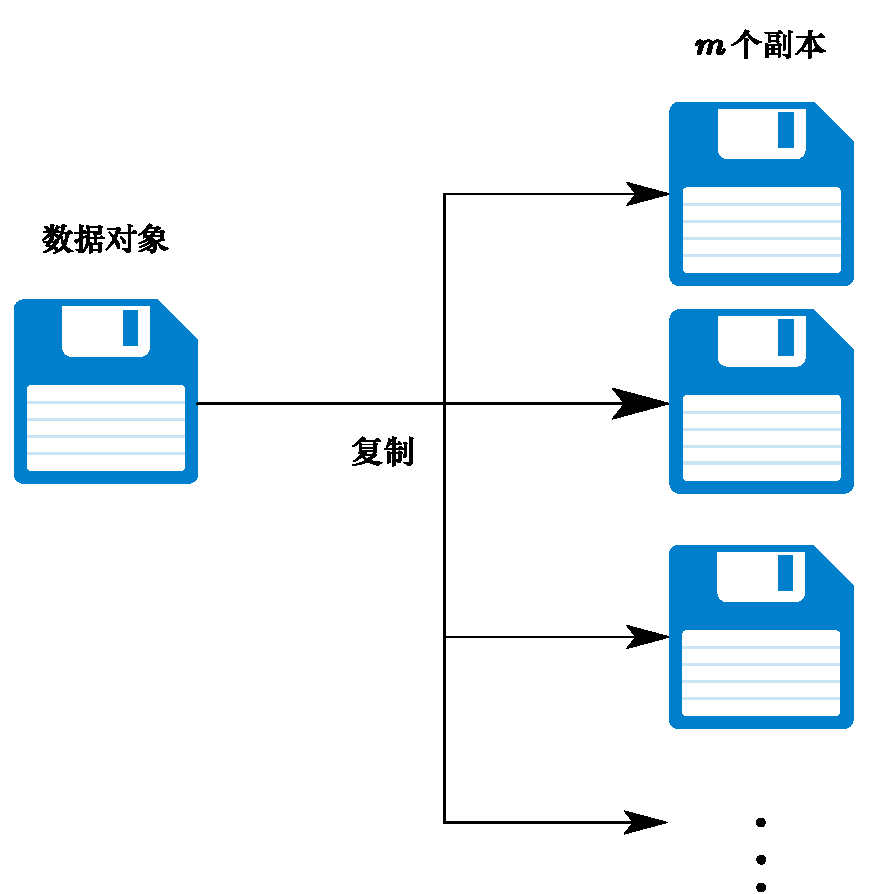
\includegraphics [scale=0.5]{figures/1.1.pdf}
	\caption{基于复制的容错机制原理}
	\label{fig:con-1.1}
\end{figure}

基于复制的容错机制原理如图~\ref{fig:con-1.1}所示,将原始数据复制多份,创建多个数据副本并分发到不同的存储节点上
从而实现数据冗余\cite{shvachko2010hadoop,ghemawat2003google,王意洁2017分布式存储中的纠删码容错技术研究}。
当一个或者多个存储着原始文件副本数据的存储节点故障时,系统通过访问其他存活节点的原始文件的副本数据,进行数据的恢复,
进而提高系统的可靠性。基于复制的冗余机制原理较为简单,易于部署和实现,并且在确保数据可靠性的基础上还能提高数据的并发访问能力。
然而,缺点显而易见,在文件储存过程中,需要分发多个多个数据副本,因此提高了数据的存储开销和通信数据的开销,存储效率较低。
对于$n$副本的复制容错机制,系统存储空间的总体利用率只有$\frac{1}{n}$。在此基础之上,为了提高存储效率,降低存储空间的开销,
可以采用动态复制机制,依据系统的网络状况、用户需求等因素进行综合考量并进行动态创建与删除副本\cite{lakshman2010cassandra,gill2016dynamic,gai2012design}。
但是,动态复制技术也存在其固有的缺陷,因为在动态创建与删除副本的过程中,需要CPU执行大量的计算,并且需要进行频繁的数据分发,从而
增加了系统的计算开销和通信开销。


相对应的,基于编码的容错机制首先对原始数据文件进行切块,再对切成的块文件进行编码,
生成体积较小的编码块从而提高数据可用性。
基于编码的容错机制生成的编码块体积小、数量少,因此,相对于基于复制的容
错机制,具有较小的存储开销。基于编码的容错机制可以分为两种:RAID技术、纠删码容错。

RAID技术\cite{patterson1988case,chen1994raid}是一种传统的基于编码的容错技术,RAID技术实现容错的方式
是通过将数据进行条带化,然后将数据条带分发到不同的存储节点上,并生成一个编码块进而实现数据的容错与冗余。
RAID技术一般只能容忍一到两个数据块的失效,因此对于大规模的分布式存储系统而言,RAID技术无法满足其数据可靠性的要求。

更加主流的基于编码的容错方式便是纠删码技术,其本身是一种编码容错技术,最早被应用到通信领域,解决数据
在传输中的纠错问题。传统的纠删码技术实现容错机制的步骤一般如下,首先将原始数据文件分割成$k$个数据块,
然后将这些数据块通过相应的矩阵计算进行编码生成$n-k$个编码块,最后将生成的$k$个数据块和$n-k$个编码块分发到
不同的存储节点中。当用户访问存储系统下载数据时,只需要从$n$个数据块中任意下载$k$个可用的块即可恢复出完整的
原始数据文件。

相较于基于复制的容错技术即多副本技术,纠删码技术最大的优势是能够以极低的存储空间开销代价换取相同甚至更高级别的
数据可靠性\cite{lin2004erasure,weatherspoon2002erasure}。例如,RS(12, 10)码可以凭借0.2倍的额外存储空间开销
获取两个节点的容错能力,这比具有同等容错能力的三副本技术节省了约60\%的存储空间。在同等的存储空间利用的情况下,
以纠删码技术构建的分布式系统的数据可靠性比采用多副本技术构建的分布式存储系统中的数据可靠性要大几个数
量级\cite{lin2004erasure,weatherspoon2002erasure}。
尽管有很多代表性的工作\citep{huang2019lower,xu1999x,reed1960polynomial,roth1989mds}对于纠删码的计算性能进行了优化,
但是纠删码方案由于其固有的缺陷如大量的矩阵计算编解码操作,依然会产生巨大的通信开销。因此如何提高纠删码容错的效率是一个亟需解决的重要问题。

\section{纠删码概述}
近年来,越来越多的大规模存储系统采用了具有较强容错能力和空间利用率较高的纠删码实现系统冗余\citep{xia2007robustore,kubiatowicz2000oceanstore}。
随着时代发展,数据规模越来越大,如何提升纠删码的容错能力用以满足系统的存储和访问需求已然成为学界与业界广泛关注的问题。

纠删码的主要思想是把一个数据对象$D$分为$k$个相同大小的数据块,通过一定的矩阵计算和编码算法生成
$n$个块($n>k$),使得通过其中任意$k'$个块即可重新还原出原始数据,具体过程如图~\ref{fig:con-1.2}所示。

\begin{figure}[tb]
	\centering
	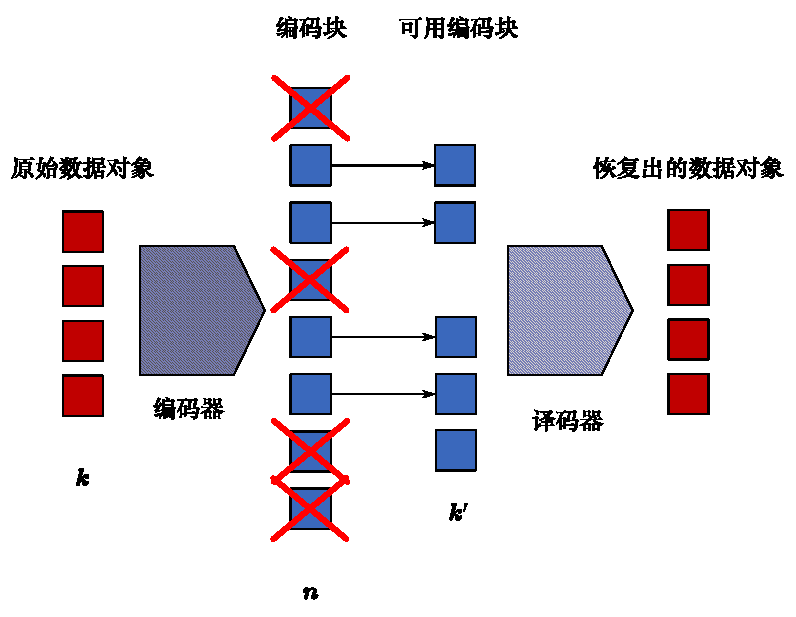
\includegraphics [scale=0.8]{figures/1.2.pdf}
	\caption{纠删码编码和解码示意图}
	\label{fig:con-1.2}
\end{figure}







一般来说,纠删码可以用三元组$(n,k,k')$表示。其中$k$是数据切分成的数据块个数,$k'$是一个不小于$k$的数,
$n$是编码后的块数。首先,将数据对象$D$分割成$k$个大小相等的数据块$D_1,D_2,...,D_k$,然后通过
编码算法和矩阵运算将这$k$个数据块进行编码,生成$n$个同等大小的编码块$I_1,I_2,...,T_n,n>k$,使得
通过其中任意$k'$个块都能还原出原始的数据对象$D$的对应的$k$个数据块$D_1,D_2,...,D_k$,从而组合出原始的数据。
纠删码可以容忍的最多失效块的个数称为容错度,当$k=k'$时,纠删码达到理论上的最高容错力,称之为最大距离可分码
(Maximum Distance Separable,简称MDS码)\cite{blaum1996mds}。这样的纠删码可用二元组
$(n,k)$表示,如果纠删码生成的$n$个块集合中包含全部的$k$个原数据块,这样的纠删码便是系统码(System Code)\cite{plank2009raid}。
对于系统码而言,编码后生成的额外$n-k$个块称为编码块,并且记为$P_1,P_2,...,P_m$,其中
$m=n-k$。如果数据块没有丢失,应用系统码的存储系统在相应数据访问操作时无需进行解码操作,性能大大提升,这也是现有的纠删码大多是系统码的原因。

在存储系统实际的运行过程中,先将文件分割成固定大小的数据块,再将这些数据块每$k$个作为一组,每组
独立进行编码操作生成$n$个块,其中$n$个块的集合称为一个条带(Stripe)\cite{hafner2005matrix},
$k$称为条带长度(Stripe Length)。当数据对象的块数不是$k$的整数倍或者最后一个数据块不足一个整块时,以0填充,被0填充的部分不需要存储在真正的磁盘上,
在数据修复时也不需要读取。根据计算方式和几何构造的不同,纠删码可分为Reed-Solomon码、阵列结构型纠删码、
网络编码型纠删码和分组结构型纠删码。

\subsection{Reed-Solomon码}
Reed-Solomon码\cite{reed1960polynomial}是最为经典的MDS码,是唯一可以用任意的数据磁盘数目和任意冗余磁盘
数目的MDS码。RS码的编码原理是通过矩阵的运算来完成的,如果分布式存储集群采用的是结构为
$(k+r,r)$的RS编码,则整个分布式存储集群应具有$k$个数据块和$r$个编码块。
在基于RS编码的分布式存储集群中,如图~\ref{fig:con-1.3}所示,编码块是通过将$k$个数据块
与$k\times (k+r)$个生成矩阵相乘来构造的,该生成矩阵主要包含了两个变量,一个
$k \times k$校验矩阵和一个$k \times r$冗余矩阵\cite{li2016procode}。一个由$(k+r,r)$
组成的RS编码存储集群,含有$k+r$个存储节点的阵列,其中$k$个数据块和$r$个编码块分别存储在存储集群中的
$k$数据节点服务器和$r$个奇偶校验节点服务器上。

\begin{figure}[tb]
	\centering
	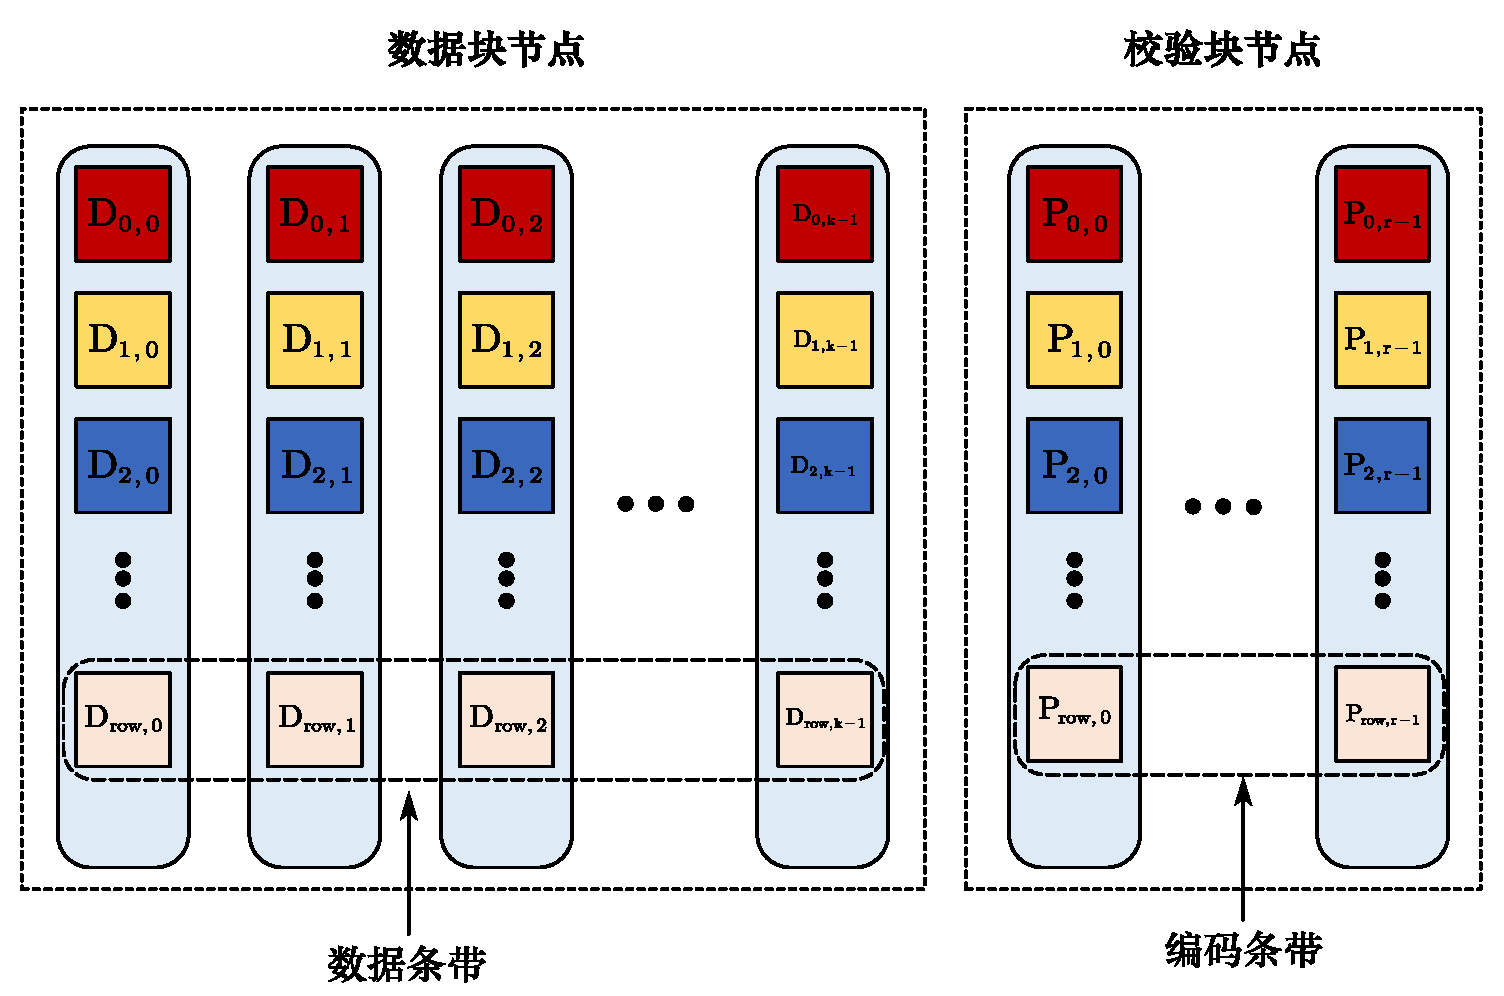
\includegraphics [scale=0.5]{figures/1.3.pdf}
	\caption{传统基于RS码结构的存储集群布局}
	\label{fig:con-1.3}
\end{figure}

RS码实际上是利用生成矩阵和数据列向量进行矩阵乘法得到编码列向量。
RS码使用的生成矩阵$G$中的任意$k$行组成的矩阵需要在Galois域上可逆,故获得生成矩阵的计算量并不低,且可由范德蒙德(Vandermonde)矩阵或柯西(Cauchy)矩阵\cite{roth1989mds}通过变换得到。
采用前者计算方法的RS码称为范德蒙德RS码,采用后者计算方法的RS码称为柯西RS码。在Galois域上,加法的定义是异或运算,
乘法则需要使用离散对数运算和查表,因此计算开销很大,而应用柯西矩阵可将乘法运算转化为二进制
的乘法运算,从而减轻运算量。

RS码拥有比传统多副本容错更高的容错能力和更高的灵活性。RS码不仅达到了理论上的最高
容错能力,而且其条带长度$k$可以取任何大于0的整数,编码后产生块数$n$可以
取任何大于$k$的整数。$n$相对于$k$越大,RS码的容错能力越高,但存储空间消耗
也越多。因此,RS码在可靠性和存储空间开销方面给予了系统很大的选择空间。

然而,纠删码的其中一个弊端在于会引起大量的带宽以及计算资源的消耗,进而导致存储效率的降低。由于计算能
力的限制,RS码从诞生起其编解码算法就已被广泛研究和优化,计算复杂
度高的问题已被较好地解决。近年来各种硬件的计算能力的显著提升,在分布式存
储系统中进行编解码运算并不会占用过多的计算资源。与RS码在信道中纠错时不
同,当RS码作为分布式存储系统的数据容错技术时,由于其产生的$n$个编码块必
须分别放在$n$个不同的节点上,若只有一个丢失,在进行数据修复时也需
要从不同节点下载$k$个编码块。这是多副本技术中修复一个块需要数据量的$k$
倍,会占用大量的网络资源,并极大地降低了修复速度。

RS码高昂的修复成本使其在分布式存储系统中的应用有很多亟待解决的问题。
然而,RS码高容错和低空间消耗的优点对提高分布式存储系统的数据可靠性和降
低其经济成本具有重大意义。为了解决这一问题,涌现出了众多修复成本较低的纠
删码。这些低修复成本的纠删码根据其采用的基本技术可以分为三类:基于阵列结构的纠删码
、基于网络编码的纠删码和基于分组结构的纠删码。

\subsection{基于阵列结构的纠删码}
阵列码是一种采用阵列结构编码且完全基于异或运算的纠删码,从
冗余磁盘阵列(RAID)\cite{patterson1988case}技术中不断发展出来。
阵列码的含义就是将原始的数据和冗余的数据一起存储在一个二维的阵列中。
根据数据块和编码块放置方式的不同,阵列码可以分为横式阵列码和纵式阵列码。

横式阵列码(horizontal parity array codes)的特点是将数据块和相应的编码块分发到不同的数据节点上。
它的结构特点是将冗余的数据单独放到独立的磁盘中,这些磁盘也被称为冗余磁盘,
而让别的磁盘专门用于存储数据,这样做的好处是可扩展性很强。


EVENODD编码\cite{blaum1995evenodd}是最早被发表的阵列码,EVENODD码的编码块和数据块之间的计算关系
如图~\ref{fig:con-1.4}所示。其中第一列上的编码块分别由各自同一行上的其他数据块进行异或得到,
第二列上的编码块由与其直线相连的对角线上的数据块进行异或运算得到。此外,RDP\cite{corbett2004row}编码也是
一种应用较为广泛的横式阵列码,这些编码体系均对磁盘数目提出了严格的要求(要求磁盘数目必须是素数或者素数减1),
同时还要求在单个条带中的数据元素的个数必须与磁盘的数目相匹配。

除了EVENODD和RDP,其他的横式阵列码有EEO\cite{feng2010eeo},
STAR\cite{huang2008star},
RAID-6 Liberation\cite{plank2009raid}和Feng's Code\cite{feng2005new}等,
它们具有性能比较优秀的编码效率和极高的存储空间利用率。由于横式阵列码本身固有的缺陷,如写入数据总会用到冗余磁盘,
故其中的I/O流量成为了横式阵列码的性能瓶颈。


\begin{figure}[tb]
	\centering
	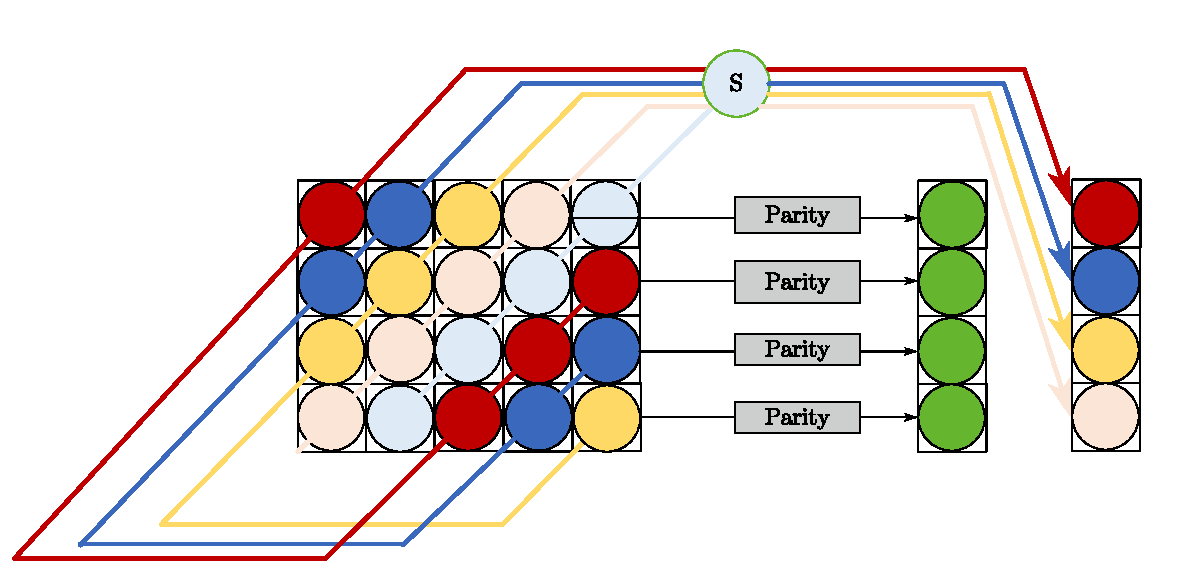
\includegraphics [scale=0.7]{figures/1.4.pdf}
	\caption{EVENODD码的编码结构示意图}
	\label{fig:con-1.4}
\end{figure}

纵式阵列码(vertical parity array codes)是指冗余存储在数据条带中的阵列编码方式,即冗余数据和原始数据
混合放在磁盘中的纠删码。由此可以看出纵式阵列码将计算工作和写入操作均匀地分摊到各块磁盘上,从而实现了
负载均衡。X-code\cite{xu1999x}是具有MDS性质的纵式纠删码,其在编码操作,数据更新以及数据重构等步骤上具有
理论上的最优效率,缺点就是可扩展性比较差。


X-code的编码方法如图~\ref{fig:con-1.5}所示,同一列上的数据块与编码块表示存储在同一个存储节点中,
存储节点上包含$k$个编码块。其中红色块代表数据块,蓝色块代表编码块,$n$需要是一个大于2的素数,数据个数必须
为$n-2$个,编码块的个数也必须是2个。此外,第一个编码块由主对角线上的数据块进行计算得到,另外一个编码块由副对角线
的数据块计算得到,这些计算需要用到$k$个磁盘上的数据块,计算成本较高,且修复时需要按照一定的顺序进行计算,失去了并行
修复的可能,这些均是X-code的不足之处。

\begin{figure}[tb]
	\centering
	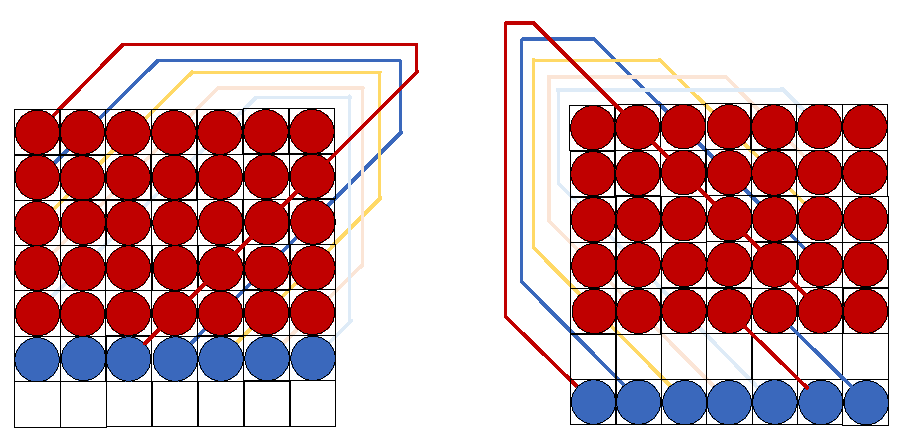
\includegraphics [scale=0.7]{figures/1.5.pdf}
	\caption{X-code的编码结构示意图}
	\label{fig:con-1.5}
\end{figure}


阵列码在计算上的主要特点就是所有的运算都是异或运算,相较于传统的RS编码在计算性能上有优化,但需要的数据量却并没有
丝毫减少,传输的数据量较大。


\subsection{基于网络编码的纠删码}
网络编码最初由\citet{ahlswede2000network}于2000年首次提出。
在传统的网络路由中,中间节点只具备存储和转发的功能。
而网络编码则增强了中间节点的功能,使得其不仅可以
存储转发数据,并且还可以在转发数据之前对数据进行编码和组合计算,从而
减少了网络中的数据传输量并提高了网络吞吐率。

\citet{dimakis2010network}将网络编码的思想应用到纠删码上并称之为再生码
(Regenerating Codes)。
再生码允许新生节点访问多于$k$个节点,从而显著降低修复过程需要传输的总数据
量。


\begin{figure}[tb]
	\centering
	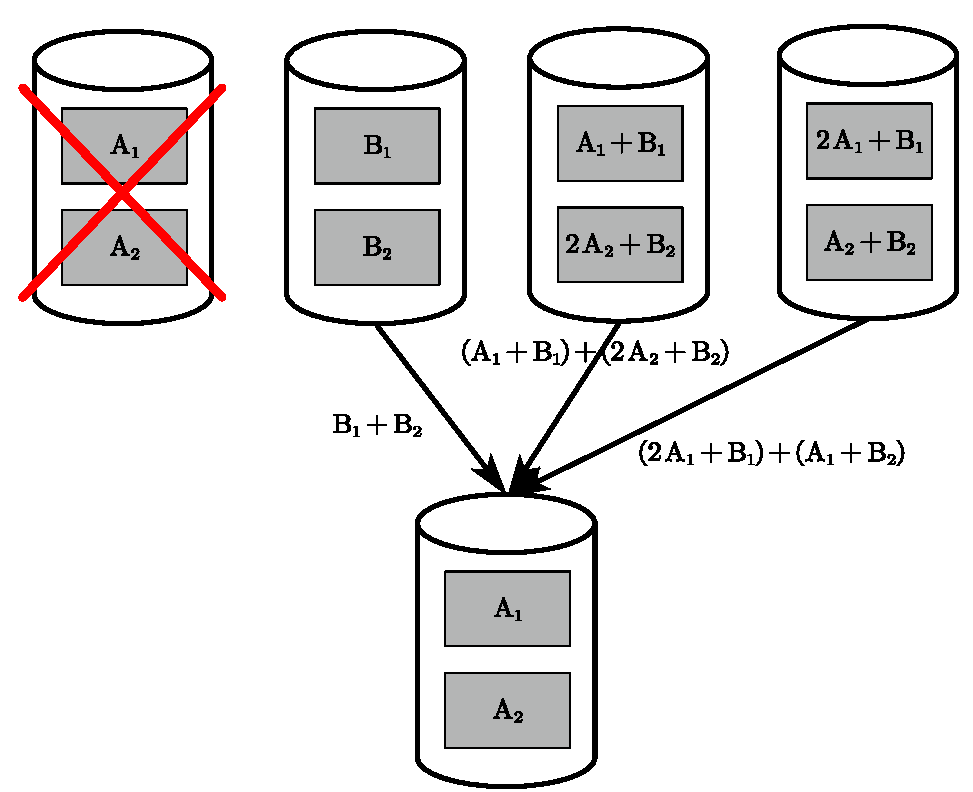
\includegraphics [scale=0.7]{figures/1.6.pdf}
	\caption{再生码修复失效数据节点示意图}
	\label{fig:con-1.6}
\end{figure}

图~\ref{fig:con-1.6}显示了再生码修复失效数据节点过程,总共有四个用来存储数据的节点,
并且每个存储
节点上存放着两个数据块,并且是通过相关的矩阵运算生成的。
若第一个存储节点发生故障时,则相应的存储的数据块会丢失。
针对此种情况,传统纠删码的修复方法是在剩下的三个存储节点中任选两个,
将这两个节点的所有数据块发送给新生节点(newcomer)
,传输数据块的总数目为4。
而再生码的思想是首先在存储节点中进行相应的计算后再进行数据分发,
传输数据块的总数目为3,相较于传统的修复方法,再生码修复数据传输量降低
了25\%。


\citet{dimakis2010network}提出的再生码可以对丢失的数据进行精确修复,
但对编码块只能进行功能性修复。
所谓功能性修复,亦即修复出的数据与原来的冗余数据并不是一模一样的,但却可以维持数据的容错度不变。
针对此问题,
\citet{wu2007deterministic}提出了确定性再生码
(Deterministic Regenerating Codes),并从概率学角度证明了其存在性。

根据存储效率的不同,再生码可以分为$\frac{k}{n}\leqslant \frac{1}{2}$的低比特率码和
$\frac{k}{n}> \frac{1}{2}$的高比特率码。它们可以在一定程度上从源头减少修复过程中传输的数据量,
但是由于编码系数所在域的要求限制和选择方法的不规则,难以实现等原因,目前应用并不广泛。


\subsection{基于分组结构的纠删码}
基于分组结构的纠删码可以减少数据修复时需要下载的数据量,因传统的RS码在修复一个丢失的块时
需要下载的数据条带长度为$k$,而分组结构的纠删码的方法则是将$k$减小从而达到降低数据量的目标。
分组编码的纠删码首先将数据条带分成若干组,各个组各自计算相应的编码块,实现组内修复丢失块,需要的块数
则取决于每个组内的数据块数。而相应的,RS码作为一种特殊的分组编码,将整个数据条带作为一组,此外根据
分组方法的不同,此类纠删码可以分为两类:水平分组结构的纠删码和交叉分组结构的纠删码。

比较经典的水平分组纠删码一般是将数据条带分为两组。每个小组生成一个局部的冗余块,然后整个条带
再生产一个全局的冗余块。这样数据修复就可以依靠小组内的编码块完成,降低了修复成本。图~\ref{fig:con-1.7}显示的是微软的
Azure系统\cite{calder2011windows}采用LRC(Local Reconstruction Codes)\cite{huang2012erasure}
的一个实际的例子LRC(8,2,2)。可以看出,它将数据块平均分为了两组,每组各自内部计算出一块局部冗余编码块,
相当于一个RS(5,4)码。对于两个条带再生成2个全局的校验块,则相当于一个RS(10,8)码。当丢失块数不多时,如1个则只需要4个块即可进行数据修复,
这样就有效降低了修复成本。

\begin{figure}[tb]
	\centering
	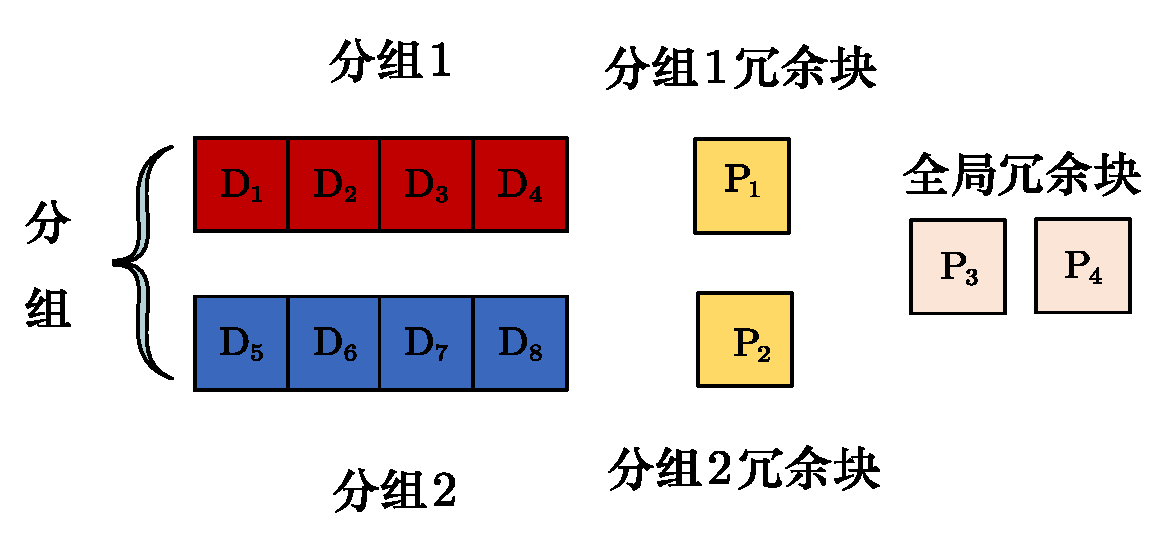
\includegraphics [scale=0.5]{figures/1.7.pdf}
	\caption{LRC(8, 2, 2)的编码示意图}
	\label{fig:con-1.7}
\end{figure}


由此可以发现,组数越多,那么可以容忍的失效的块数也就越多,故Pyramid码\cite{huang2013pyramid}便诞生了,
它的特点就是可以对条带内的数据块进行任意层次的分组,层次越多平均的修复成本也就越低,但是相对的存储空间消耗也就越大,
因为产生了更多的全局校验块,对于Pyramid码需要根据实际的存储系统环境选择更加适中的方案。除此以外水平结构
的编码还有运行在Facebook旗下的分布式存储系统中的XORing Elephants\cite{sathiamoorthy2013xoring}、
EXPyramid\cite{周松2011expyramid}、LRCs\cite{sathiamoorthy2013xoring}等。EXPyramid码是对两层
Pyramid码的一种改进,其分为了三组。

交叉分组结构的纠删码与水平分组不同之处大致有两点。第一,交叉分组纠删码的分组方式不同,交叉分组
的各组之间相互重叠但却互不包含,相比之下水平分组各组之间一般不重叠且会有一个全局的校验块包含着各个分组的校验块。
第二,交叉分组纠删码编码计算较为简单,基于异或计算。不难看出,交叉分组有着相对来说较低的计算性能消耗的优点。常见的交叉结构的
纠删码有\citet{woitaszek2007tornado}提出的Tornado码,如图~\ref{fig:con-1.8}所示,其任何组别的荣愉快均为组内的数据块的校验块,并且
修复任何一个数据块或者冗余块只需4个或3个块,避免了大量下载编码块的特殊情况。此外还有
LDPC\cite{gallager1962low}、WEAVER码\cite{hafner2005weaver}和Tanner码、Hover码\cite{hafner2006hover}等。


\begin{figure}[tb]
	\centering
	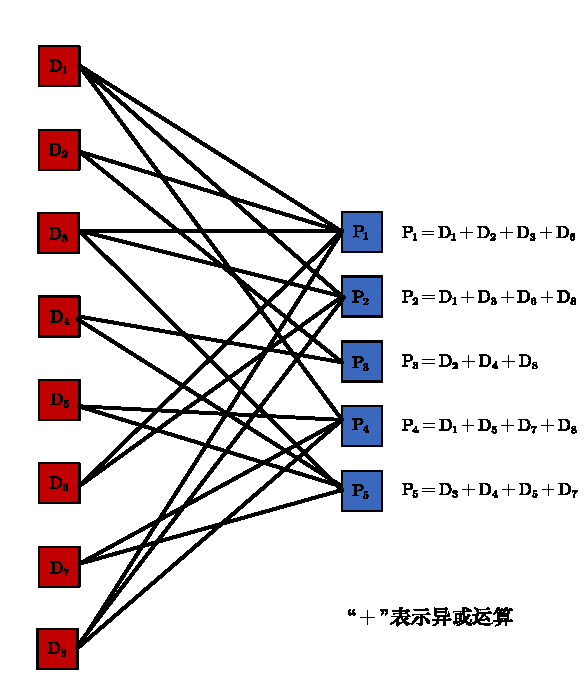
\includegraphics [scale=0.7]{figures/1.8.pdf}
	\caption{Tornado码的构造示意图}
	\label{fig:con-1.8}
\end{figure}




\section{基于纠删码的数据修复技术}
在基于纠删码的分布式存储系统中,数据传输并不是简单的线性路线,修复一个丢失的数据块时,
提供者节点要向新生节点传输多个数据块用以完整地修复数据,数据的传输路径往往比较多样化,根据传输
路径的不同一般可分为三种修复技术:基于星型拓扑的数据修复、基于树型拓扑的数据修复和基于XOR的纠删码数据修复。

\subsection{基于星型拓扑的数据修复}
基于星型拓扑的串行修复技术(Star Structure Based,SSR)是指依序逐个修复故障的节点数据,每个故障
节点的修复过程都是按照星型拓扑来进行的。具体来说,以新生节点为中心,各个存活节点之间并不相互传输数据,
存活节点直接向新生节点传输数据,从而形成了一个以新生节点为中心、存活节点为边界的星型拓扑结构。
可以看出,修复的时间取决于新生节点与存活节点之间最慢的一条带宽链路。

\citet{dimakis2010network,wu2007deterministic}提出的再生码数据修复过程要求每个存活节点向
新生节点传输均等的数据量进行修复,数据收集节点(DC节点)仅连接$k$个节点,通常
是$k-1$个数据节点和第一个校验数据节点,并从每个节点下载$\frac{M}{k}$的数据量($M$为原文件大小)。这里存在一个
非常明显的缺陷,节点可以选择的链路比较单一,带宽较高的链路很有可能会被忽视,导致修复效率降低。
\citet{shah2010flexible}提出了弹性修复的方法,即允许存活节点和DC节点充分利用所有可用的链路,
从中选择带宽较大的链路进行数据传输,传输的数据不均等。DC节点从节点$i(1 \leqslant i \leqslant n)$
下载$\mu_i (0 \leqslant \mu_i \leqslant \alpha)$,满足总下载量不小于$M$即可。同理,新生节点从存活节点
$i(1 \leqslant i \leqslant n)$接收$\beta_i (0 \leqslant \beta_i \leqslant \beta_{max})$
数据量,满足总接收量大于或等于一个设定参数$\gamma$即可,用不等式表示
则如~\ref{eq:1-1}和~\ref{eq:1-2}:

\begin{equation}
	\label{eq:1-1}
	\sum_{i=1}^{n} \mu_{i} \geq M, 0 \leq \mu_{i} \leq \alpha
\end{equation}
\begin{equation}
	\label{eq:1-2}
	\sum_{i=1}^{n} \beta_{i} \geq \gamma, 0 \leq \beta_{i} \leq \alpha
\end{equation}

当一个节点故障时,新生节点可以选择任意$k$个节点下载$\frac{M}{k}$的数据量,修复带宽相等于原文件大小。
对于弹性修复方法而言,新生节点,可以根据可用带宽的大小从不同节点上下载不均等的数据来降低修复时间。
当然星型拓扑的缺点也很明显,DC节点需要收集多个节点的数据,修复速度会受到磁盘和网络I/O的限制,编解码的计算消耗也很大。

\subsection{基于树型拓扑的数据修复}
上节所描述的星型拓扑的技术其实是树型拓扑修复技术的特殊情况,然而修复速度受到了诸多的制约,为了提升修复的速度,
树型拓扑修复方法因此别提出。


\subsection{基于XOR的纠删码数据修复}

\section{纠删码及修复技术的问题和挑战}

\section{论文主要研究内容}

\section{论文组织结构}




% 中文参考文献\cite{li-2013-chinese-dep}

% 英文参考\cite{krahenbuhl-etal-2011-efficient}



\chapter{相关研究}

\section{基于感知修复的研究现状}
\section{基于改进纠删码结构存储数据研究现状}
\section{基于调度优化的数据修复研究现状}
\chapter{纠删码的高可靠预先数据修复算法研究}







\section{引言}

分布式存储系统通过对数据进行冗余来保证数据的可靠性和可用性,基于纠删码的冗余技术能减少存储空间。
在存储集群中利用多个节点来提供足够的数据冗余以降低数据丢失的可能性。
多备份冗余是创建了至少三份数据副本,但是在数据存储急剧增长的情况下,
备份冗余会引发大量存储开销,早期的分布式集群一般采用这种方式.
纠删码则是通过编解码矩阵的计算创建了远小于多备份技术的冗余数据,
同时提供同级别的容错性\cite{weatherspoon2002erasure}。如今的大规模存储群越来越多地采用纠删码\cite{ford2010availability,huang2012erasure,muralidhar2014f4,ovsiannikov2013quantcast},
以取得存储空间和可靠性的均衡。

纠删码面临的最基本问题就是过量的修复开销:
修复流量随着存储冗余度的降低而增加\cite{dimakis2010network}。因此,前人对改善纠删码的修复性能进行了广泛的研究,
使修复过程中的修复流量或I/O最小化\citep{dimakis2010network,huang2012erasure,sathiamoorthy2013xoring},
或设计适用于所有实践中的纠删码包括RS码的提高修复效率的技术\citep{bhagwan2004total,li2017repair,li2019openec,mitra2016partial,shen2016reconsidering,silberstein2014lazy}。
目前,大部分的传统修复方法都是被动修复,只有在检测到节点故障后才会触发修复操作。
如果可以提前预测即将发生的故障,就可以在任何实际故障发生之前主动修复任何即将发生的节点故障,以提高系统可靠性。

随着机器学习技术的不断发展,很多研究也将其与磁盘预测技术结合在一起进而提高预测精准度。
在某些情况下,预测精度甚至可以达到至少95\%\cite{botezatu2016predicting,li2014hard,mahdisoltani2017proactive,zhu2013proactive},
并且误报率非常小。故\citet{shen2019fast}定义了STF节点为根据预测技术得到的精确的即将故障的节点,在这前提下
通过耦合两种修复方法——迁移和重建提出了FastPR算法,准确定位STF节点并加速修复操作。然而在修复调度上,FastPR在带宽快速变化的网络环境中,尤其是在
带宽不对等的环境下修复性能会受到限制。

本文在FastPR对于STF节点修复任务的前提下, 进一步将其扩展到网络环境快速变化的情形中。利用空闲节点加速数据的传输并感知当前网络环境的变化。

\section{预先修复问题建模}
本文通过结合迁移与重建来设计实现预先修复的机制,用以修复STF(Soon To Fail)\cite{shen2019fast}节点。
这两种修复方式各有其优缺点,迁移是直接从一个STF节点上读取存储的编码与数据块,将其重新传输到一个或多个正常的节点中,
与常规读取相比,它并不会引发额外的带宽消耗。然而,迁移的性能却受到STF节点可用带宽的限制,另一方面,
重建修复遵循着传统的反应式修复,亦即只有当节点数据不可访问时才会触发修复机制,
通过从可用节点中检索多个条带来重建STF节点的数据条带。由于这些数据与编码条带通常分布在存储集群中,
可以利用存储集群的可用带宽资源,让所有可用节点以并行的方式参与STF节点的多个条带的修复,但是会引发额外的带宽消耗。

\subsection{问题描述}

以$RS(5,3)$为例,其中$n=5$和$k=3$,设$N_i$为第$i$个可用节点,
$S_i$是要修复的STF节点的第$i$个块的条带。假设现在得到了一个STF节点的$c_m$和$c_r$的集合,
其中$c_m$为迁移的块的个数,$c_r$为重建的块的个数。如图~\ref{fig:3.2}所示的存储集群,总共有$M=7$个节点,其中$M-1=6$个可用节点,
$N_1,N_2,\cdots,N_6$,而STF节点的块对应于条带$S_1,S_2,S_3$。


\begin{figure}[htbp]
	\centering
	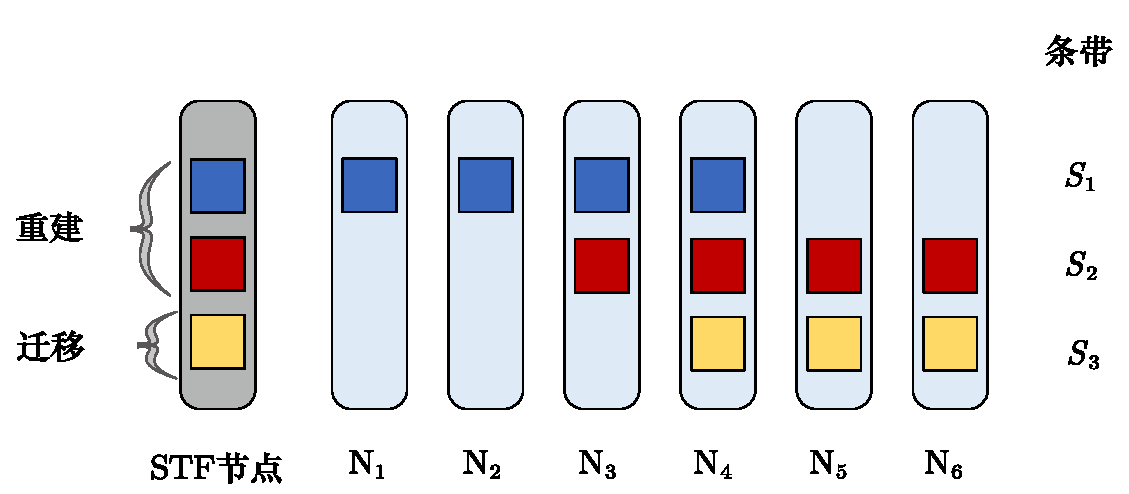
\includegraphics [scale=0.5]{figures/3.2.pdf}
	\caption{RS(5,3)的条带分布}
	\label{fig:3.2}
\end{figure}

\citet{shen2019fast}提出,对于这样的通常情况需要解决两个基本问题,
其一是在给定的通过重建修复的STF节点的$c_r$块中,
需要确定从$k-c_r$个可用节点中检索出$k-c_r$个块,将$k-c_r$的检索选择表述为一个二分图最大匹配问题。
其二是需要确定存储$c_m+c_r$个修复后的块。一般而言,将修复的块存储在$c_m+c_r$个现有的可用节点中,
这样就可以保持节点的容错性,即任何$n-k$个节点的故障都是可以容忍的,再次将选择$c_m+c_r$个可用节点表述为二分图最大匹配问题。

然而在实际分布式网络修复中,不仅仅只关注需要用到哪些块进行修复与存储,
其中并行的性能还受到节点之间的快速变化的带宽和文件访问频次的影响。
首先按照在一个存储集群中对于不同种类的数据访问频次的不同,
包含相应文件的节点宕机造成的损失要远高于存放那些不常用的数据的节点宕机所造成的损失,
这种情况在预先修复中就需要纳入考虑,提高对热数据的修复顺序的权重可以极高地增加存储集群的可靠性与持久性;
其次,对于一个STF节点而言,存储着来自不同数据的数据块与校验块,如何确定当前所需要的块的修复方法也是至关重要的。
在快速变化的网络环境中,可用节点并行地处理修复任务与迁移任务,不同节点的带宽瓶颈不同,
如果在修复过程中随机选择迁移或者重建方法,势必会造成整个网络修复性能得不到充分利用,
或者某个节点超出负荷的运行而剩下的节点却处于空闲状态,
需要设计一个算法充分利用整个网络的带宽进行重建与迁移,其中至关重要的就是对于一个STF节点确认其重建集$c_m$与迁移集$c_r$。

问题转化为计算出$c_m$和$c_r$的集合,亦即确定重建集和迁移集的具体块。
有如下具体问题,若一个STF节点拥有$m+r$个数据块,每个块对应的文件有着相应的访问热度$T_i(1\leqslant n \leqslant m+r)$,
且在可用节点中,$w_{nj}$表示$n$节点到$j$节点实时带宽速度,每个节点拥有$t$个数据块,分别为$[N_s,\cdots,N_k,\cdots,N_t](s<k<t)$,
以及每个节点是否处于参与修复任务状态位$State_n$,取值为$\{T,F\}$,现在需要确定当STF节点产生时,
其中的数据块通过耦合重建和修复达到修复时间最短的方案。

\subsection{模型假设}
修复技术的主要目标就是减少修复时间,并且最大化地利用实时带宽。为此我们做出如下假设:

\begin{enumerate}
	\item 存储集群每次最多只有一个STF节点,这是基于单节点修复是最主要的修复事件,且占据修复事件总数的98\%\cite{rashmi2013solution}。
	\item 随着系统运行,配备的预测算法预测出的STF节点的成功率是100\%。
	\item STF节点中的分块在修复过程中仍然可以访问,直到STF节点实际发生故障。
	\item 在多次修复后,块分布可能会变得不平衡,假设集群拥有自动再平衡的能力。
\end{enumerate}

\subsection{理论修复时间}
\label{subsection3.1}

设$M$为存储系统中的节点总数,$U$为STF节点需要被修复的块的总量。设$x$是被迁移修复的块的数量,则$U-x$是重建修复的块的数量。对于迁移修复,
$t_m$为将一个块从STF节点迁移到另一个正常节点的时间,因此总的迁移时间为$x \cdot t_m $。对于重建修复,
令$t_r$为修复STF节点的一个块的时间。在$RS(n,k)$的设置下,$k$个正常节点需要搜索$k$个块来重建STF节点的
每个块,若$M-1$个正常节点数远大于$k$,则可以同时重建STF节点的多个块。假设重建修复可分为多轮,那么在每一轮
中,可以找到$G\leqslant \frac{M-1}{k}$个不重叠的组,这些组中的$k$个节点属于不同的条带,并可以从这些
组并行地搜索出$k$个块。因此,可以在$t_r$时间内通过重建修复STF节点的$G$个块,重建消耗的总时间为$\frac{U-x}{G} \leqslant t_r$。

令$T(x)$为预先修复的总时间,又重建和迁移是并行执行的,则:
\begin{equation}
	\label{eq:3-1}
	T(x)=\max \left(x \cdot t_{m}, \frac{U-x}{G} \cdot t_{r}\right)
\end{equation}

当$x \cdot t_m = \frac{U-x}{G} \cdot t_r$时,$T(x)$最小,也就是$x = \frac{U \cdot t_{r}}{G \cdot t_{m}+t_{r}}$。因此,最小的
预先修复时间$T_P$为:
\begin{equation}
	\label{eq:3-2}
	T_{P}=\frac{U \cdot t_{r} \cdot t_{m}}{G \cdot t_{m}+t_{r}}
\end{equation}

对于反应式修复只会进行重建,则总的修复时间为$T_R$则为式~\ref{eq:3-1}中,当$x=0$时的$T(0)$:
\begin{equation}
	\label{eq:3-3}
	T_{R}=\frac{U \cdot t_{r}}{G}
\end{equation}

\subsection{迁移与重建时间建模}
本文将修复过程分解为三个部分,并按照顺序方式进行。(1)读取,从本地存储中读取数据块;(2)传输,通过网络进行数据传输;(3)写入,将修复后的数据写入
正常节点。设$b_d$和$b_n$分别为磁盘和网络带宽,$c$是块大小。首先对于迁移任务,对于每个块的读取时间为$\frac{c}{b_d}$,传输时间为$\frac{c}{b_n}$,
写入时间为$\frac{c}{b_d}$,则$t_m$有:
\begin{equation}
	\label{eq:3-4}
	t_{m}=\frac{2c}{b_{d}}+\frac{c}{b_{n}}
\end{equation}

对于重建任务,$k$个正常节点可以并行地读取同一条带的块,故对每一个待读取块的读取时间为$\frac{c}{b_d}$。因为接收$k$个块的节点一个时间步只能接收一个块,
故所有$k$个块的传输时间为$k \cdot \frac{c}{b_n}$,正常节点接收了所有$k$个块后进行矩阵计算(这里忽略计算时间)得出一个数据块写入正常节点,故写入
时间为$\frac{c}{b_d}$,因此$t_r$有:
\begin{equation}
	\label{eq:3-5}
	t_{r}=\frac{2c}{b_{d}}+\frac{k \cdot c}{b_{n}}
\end{equation}

设$M=100$,$U=1,000$,块大小$c=64MB$,$b_d=100MB/s$,且$b_n=1Gb/s$。考虑$RS(9,6)$,$RS(14,10)$,$RS(16,12)$三种分布式存储系统中的
常见RS码配置。如图~\ref{fig:3.1}所示,当节点数较少、$k$较大、$b_d$较大、$b_n$较小时,分别对应了~\ref{fig:3-1},~\ref{fig:3-2},~\ref{fig:3-3},~\ref{fig:3-4}四张子图,
预先修复的性能要反应式修复更加高效。
总的来说,预先修复在所有情况下都减少了反应式修复的修复时间,例如,在$RS(16, 12)$中减少了33.1\%(图~\ref{fig:3-2})。


\begin{figure}[htbp]
	\centering
	\begin{subfigure}[t]{0.4\textwidth}
		\centering
		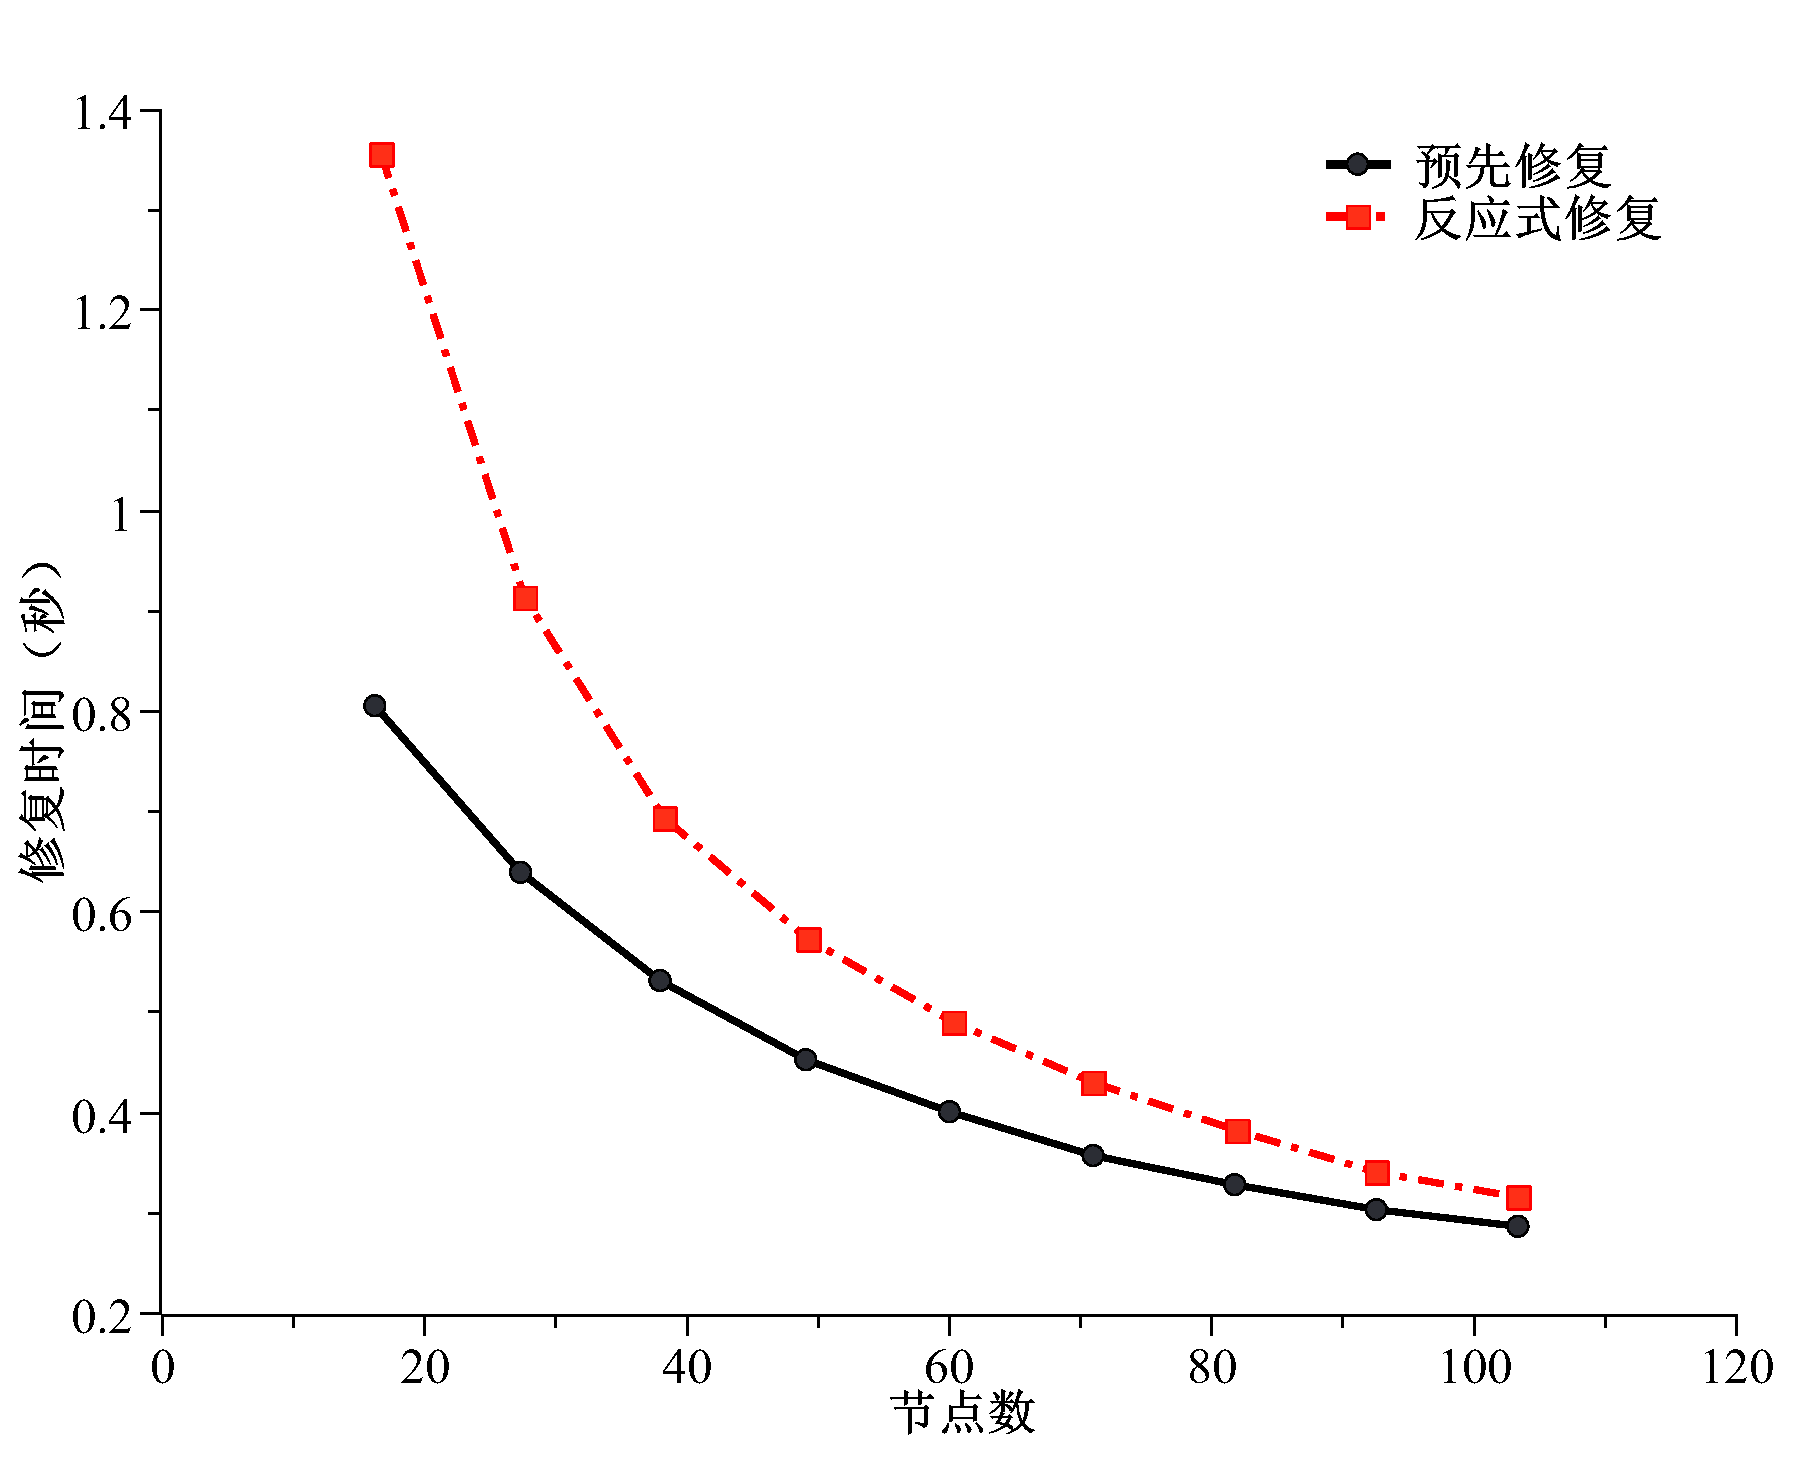
\includegraphics[width=1.1\linewidth]{figures/3-1.pdf}
		\caption{总节点数$M$值理论结果}
		\label{fig:3-1}
	\end{subfigure}
	\begin{subfigure}[t]{0.4\textwidth}
		\centering
		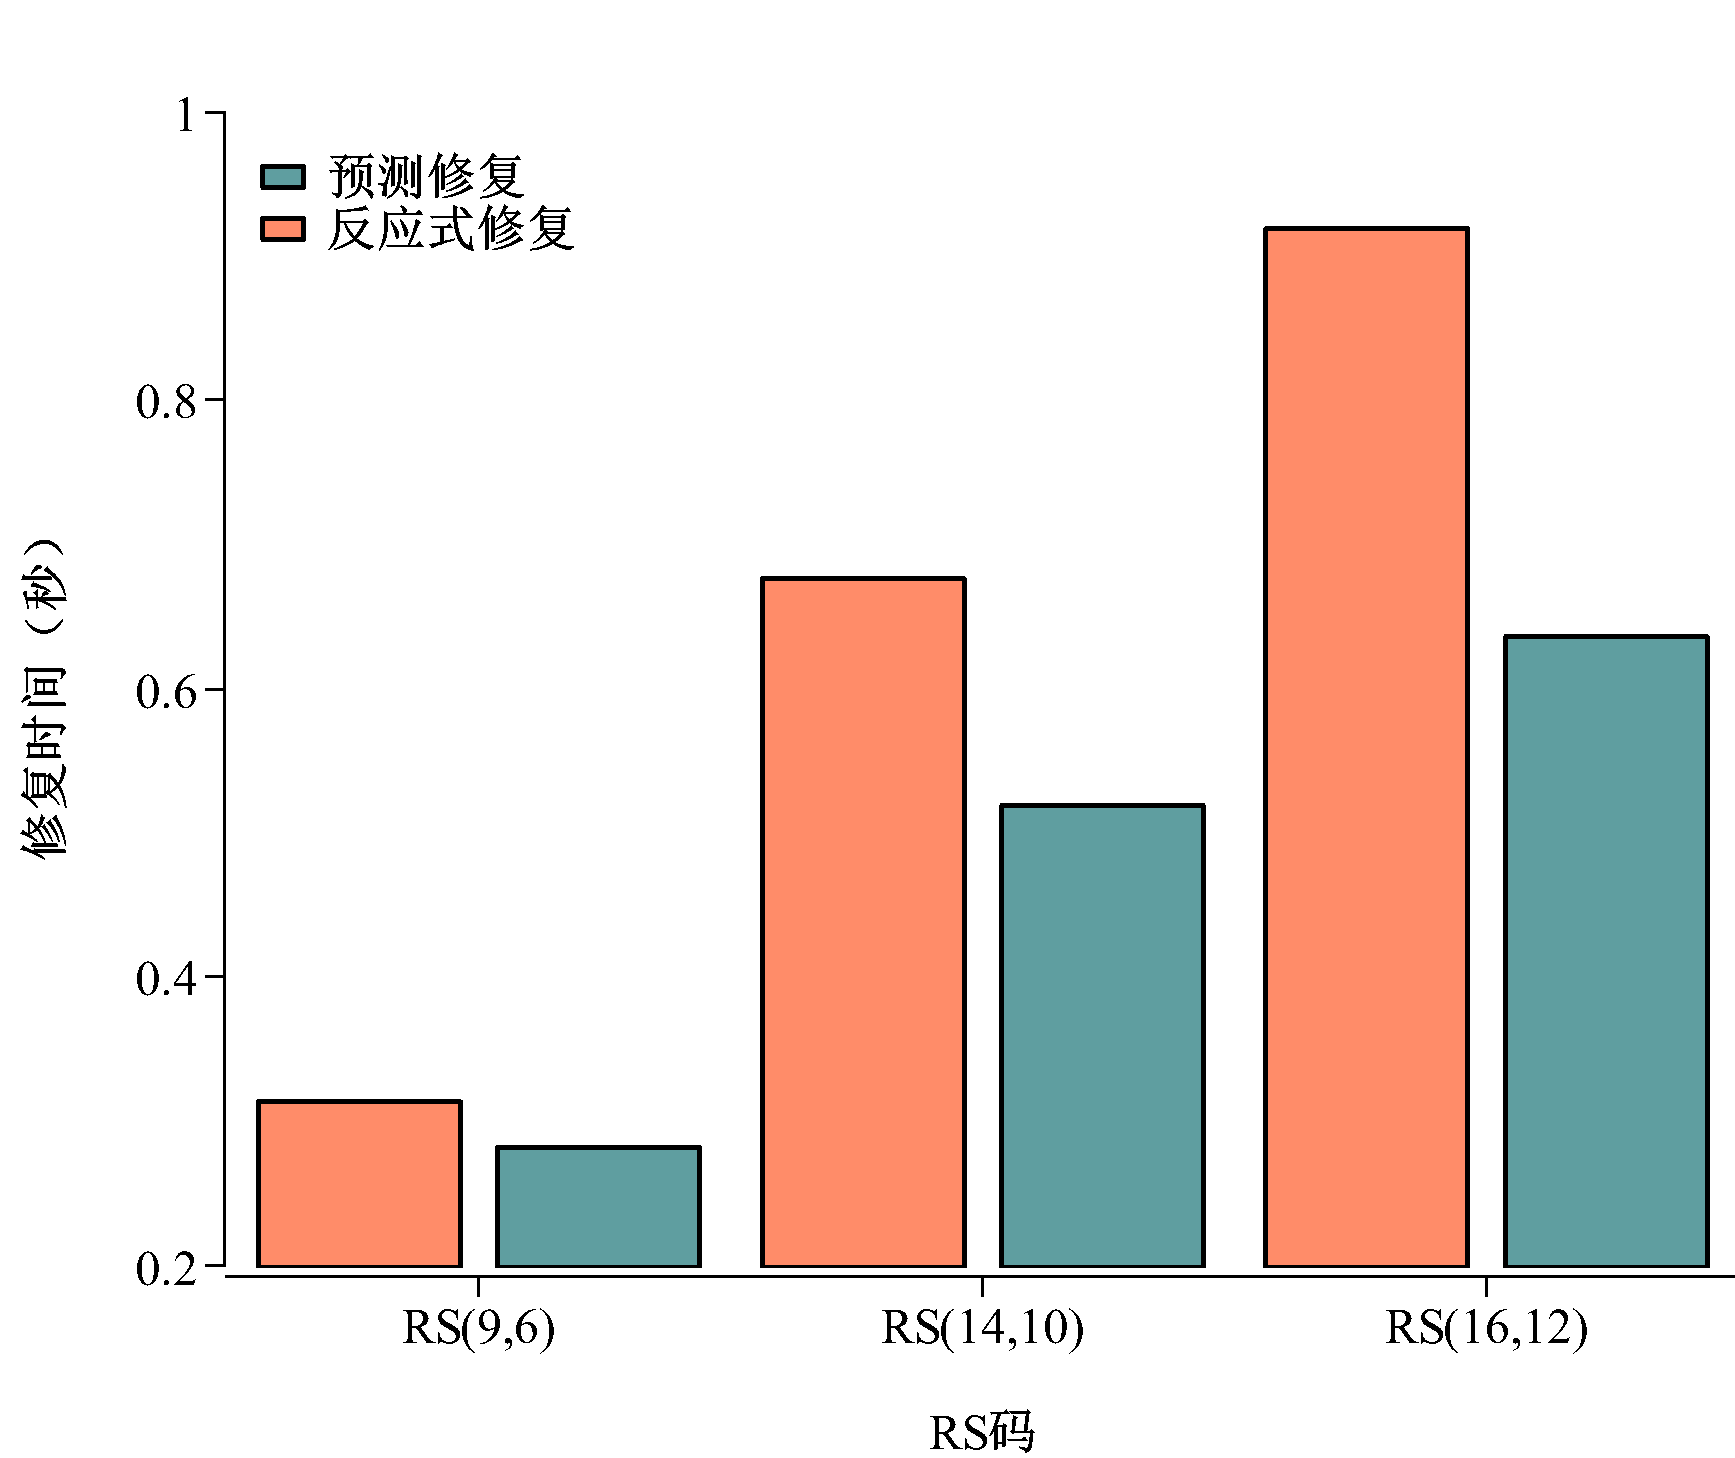
\includegraphics[width=1.2\linewidth]{figures/3-2.pdf}
		\caption{$RS(n,k)$配置理论结果}
		\label{fig:3-2}
	\end{subfigure}
	\begin{subfigure}[t]{0.4\textwidth}
		\centering
		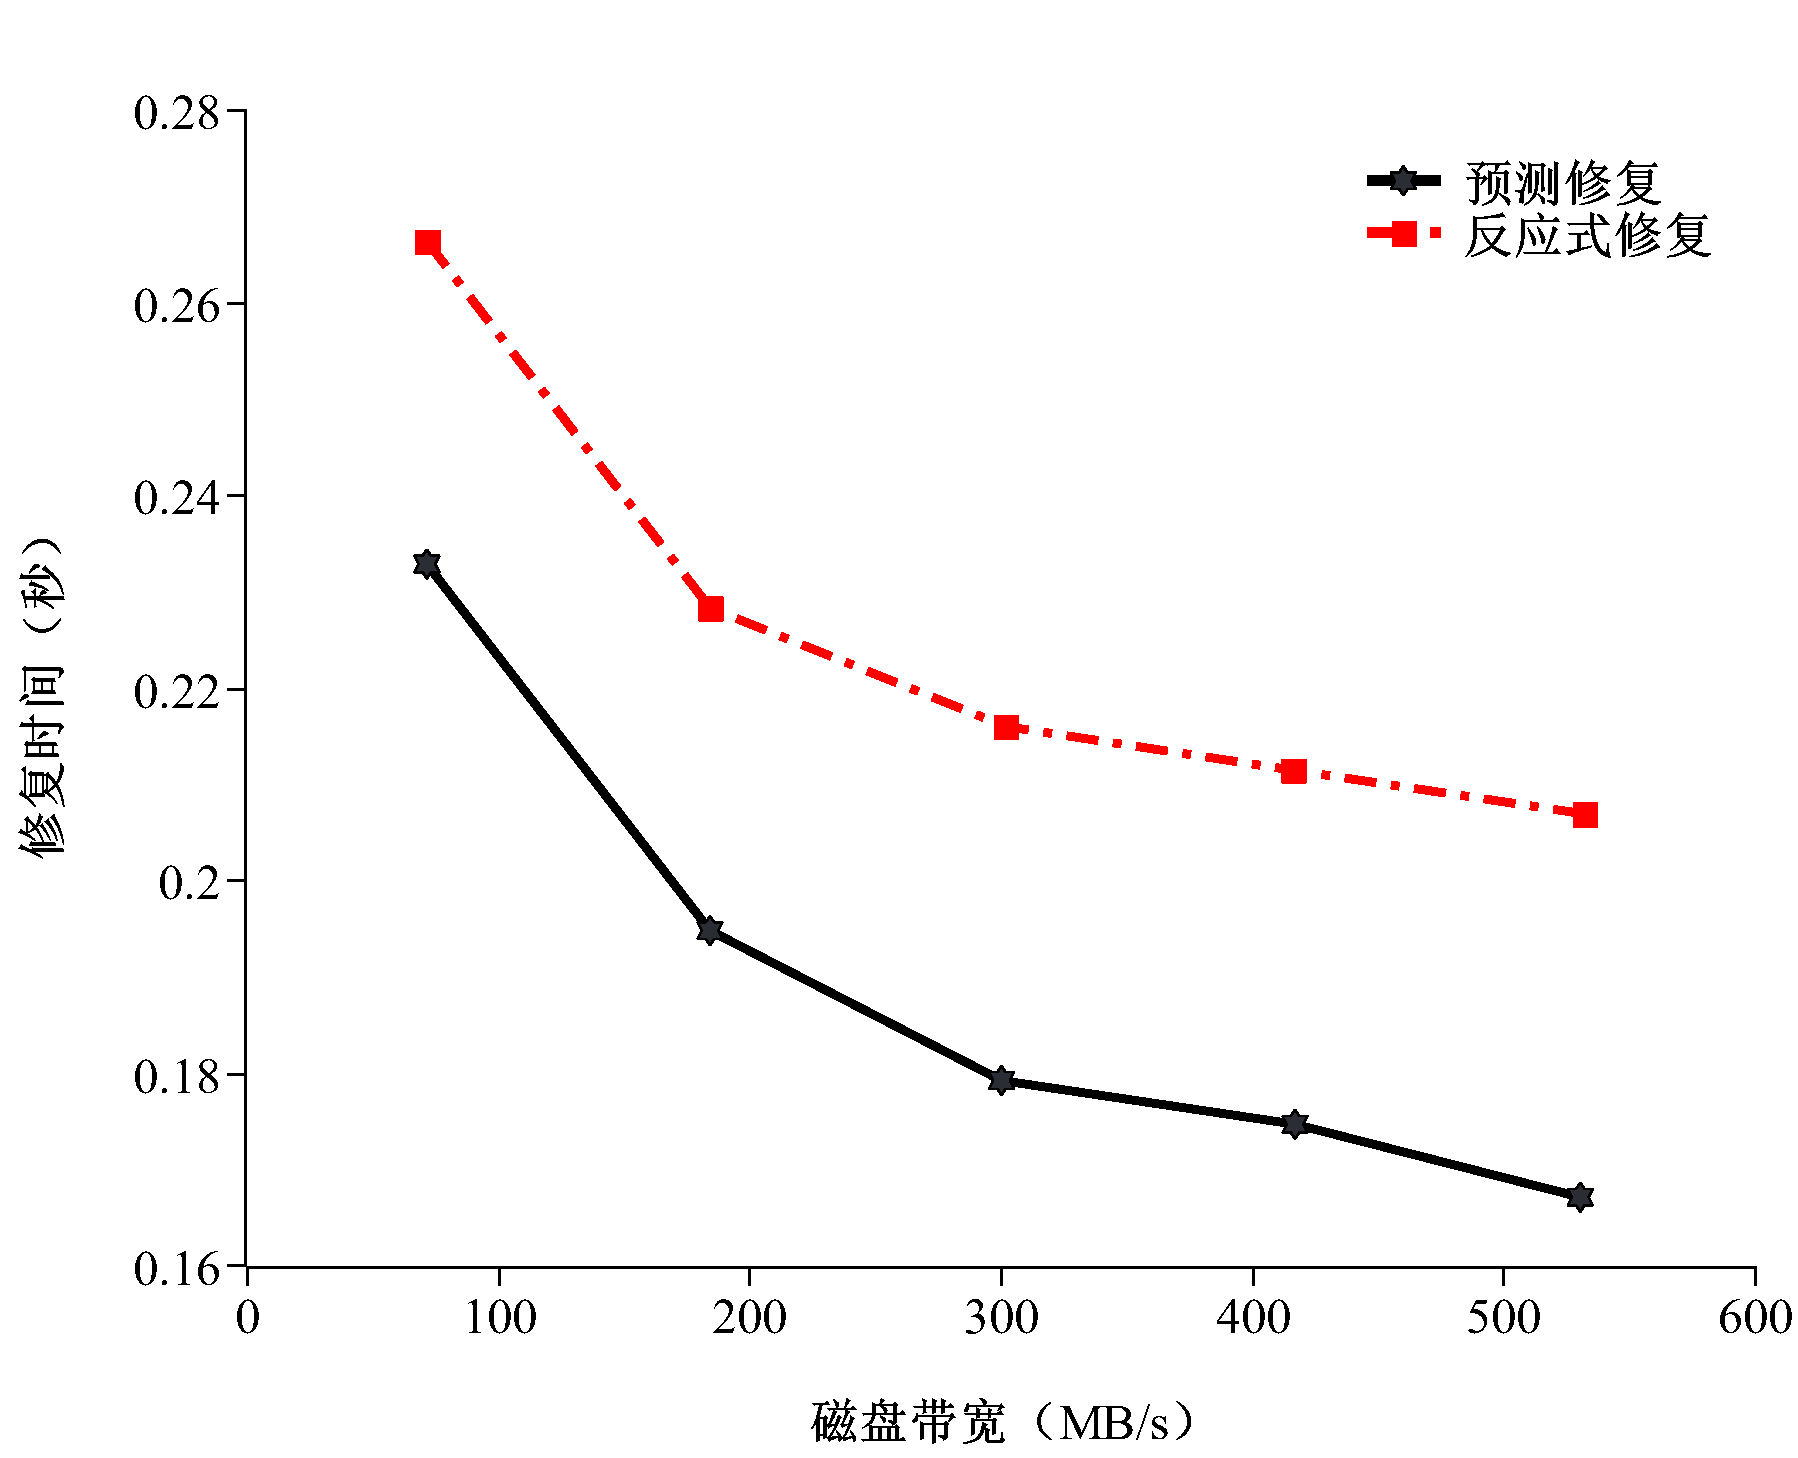
\includegraphics[width=1.1\linewidth]{figures/3-3.pdf}
		\caption{磁盘带宽$b_d$理论结果}
		\label{fig:3-3}
	\end{subfigure}
	\begin{subfigure}[t]{0.4\textwidth}
		\centering
		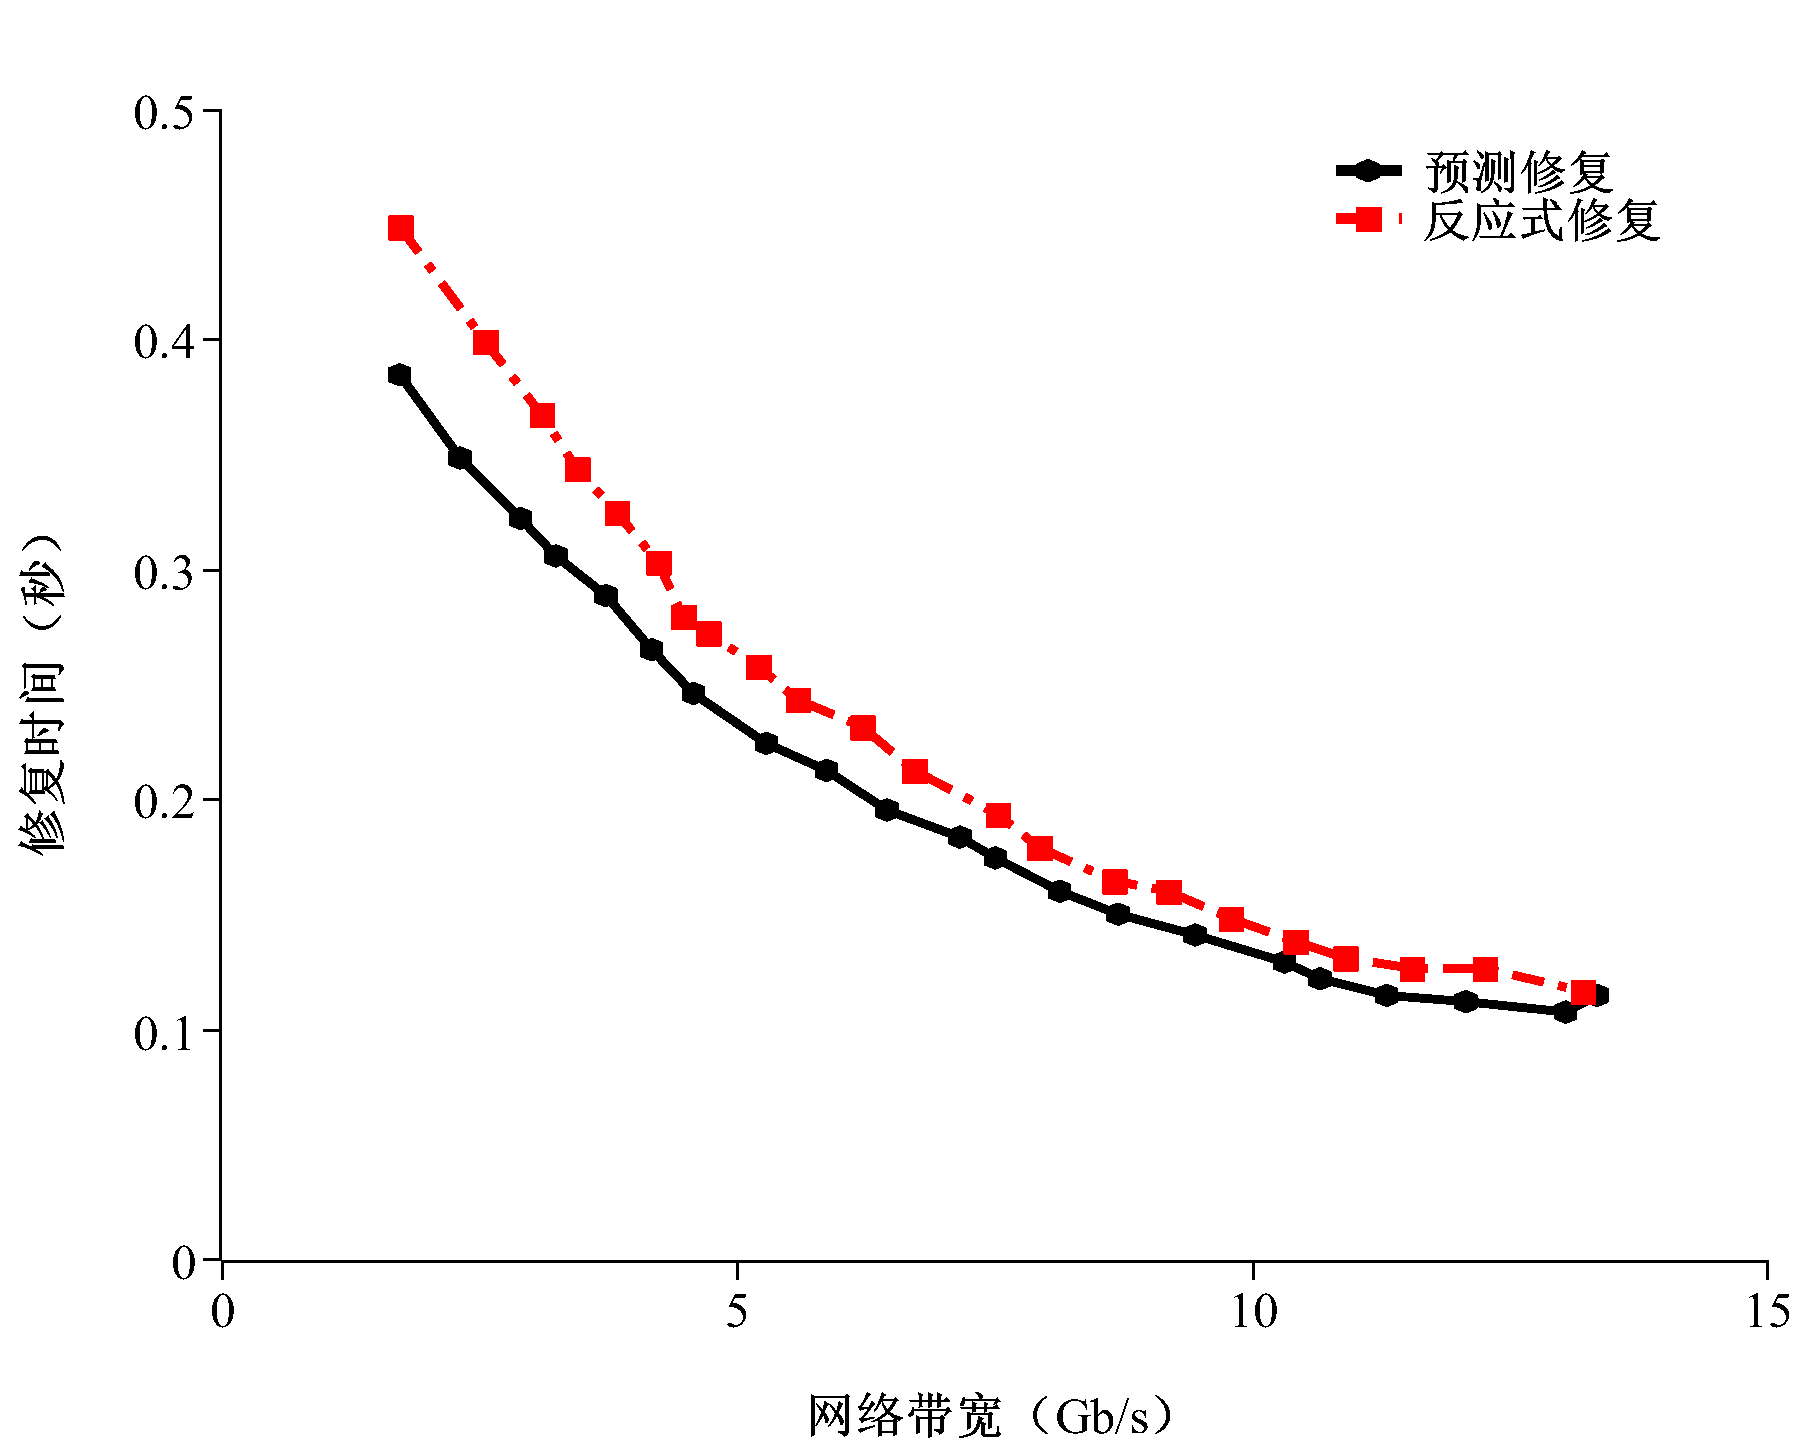
\includegraphics[width=1.1\linewidth]{figures/3-4.pdf}
		\caption{网络带宽$b_n$理论结果}
		\label{fig:3-4}
	\end{subfigure}
	\caption{预测修复与反应式修复建模对比}
	\label{fig:3.1}
\end{figure}


\section{预先修复集合划分算法}
在FastPR\cite{shen2019fast}中,算法的目标是最大限度地在每轮修复中增加STF节点的块的数量。假设STF节点中的所有块都要
通过重建方法进行修复,即从$k$个正常节点中获取$k$个块,这样中最多可以从$M-1$个正常节点每个节点获取一个块,这样就可以
在一个修复轮次中完成修复任务。
所以为了提高并行性,应该最大化重建集的块数量,如章节~\ref{subsection3.1}所说,最大为$\frac{M-1}{k}$。

如图~\ref{fig:3.3}所示,本文针对重建集与迁移集问题,设计了划分迁移集与重建集算法SMSRS(Split Migration Set And Reconstruction Set)算法,如算法\ref{alg:3-1}所示。
该算法主要使用数据热度队列与最小堆技术,根据数据访问热度高低处理待修复的块的出队修复顺序,
利用最小堆不断优化当前出堆的网络带宽性能最优的可用节点进行迁移修复,然后通过贪心策略确定最佳的重建节点以及对应的重建块接收节点。

\begin{figure}[htbp]
	\centering
	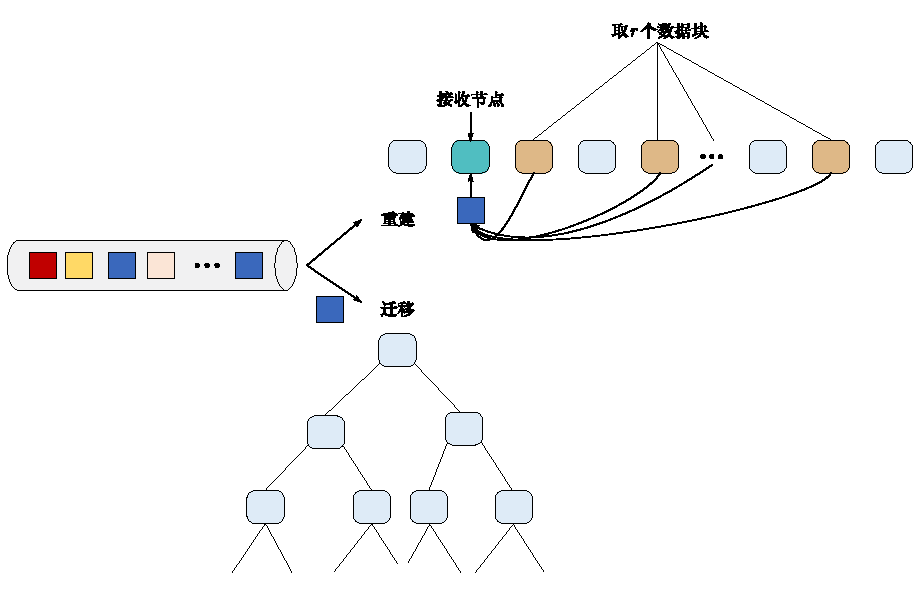
\includegraphics [scale=0.9]{figures/3.3.pdf}
	\caption{重建与迁移修复流程}
	\label{fig:3.3}
\end{figure}

在获得迁移集$c_m$和重建集$c_r$中,需要先根据文件访问热度对相应文件的数据块进行排序送入队列$Q$(第1$\sim$2行),
按照热度从高到低的顺序从队列$Q$中弹出STF节点中待修复的块,
将其对应的节点编号按照与可用节点当前连接带宽的大小进行小堆化,
这样可以保证每次在堆顶取出当前与STF节点连接带宽速度最快的节点进行修复(第4$\sim$5行)。
在可用节点中找出当前不含有该STF节点待修复块的节点集$S_1$,并且不断从堆顶取出节点编号,
判断该节点是否处于执行修复任务状态以及是否包含于节点集$S_1$,若是则跳出,然后将不满足条件但弹出堆的数据再放回堆中,
并计算通过迁移块修复所耗费的时间$t_m$(第6$\sim$16行)。在可用节点中找出当前含有该STF节点待修复块的节点集$S_2$,并且定义带宽集$\textbf{D}$,
表示的是节点集$S_2$与可用节点集$\textbf{N}-S_2$中带宽各个节点传输的实时带宽值,在节点集$S_2$确定$r$个节点,
并在可用节点集中找出与这$r$个节点连接带宽值最大的节点$RNode$,
然后得出$r$个节点中与$RNode$连接最慢的节点除以块大小即得出对应的通过重建块修复所耗费的时间$t_r$(第17$\sim$30行)。
最后通过判断$t_r$和$t_m$的大小来确定重建集和迁移集,当队列$Q$为空时,则结束整个算法,返回相应的迁移集$c_m$和重建集$c_r$(第31行$\sim$39行)。



\renewcommand{\algorithmicrequire}{\textbf{Input:}} % Use Input in the format of Algorithm
\renewcommand{\algorithmicensure}{\textbf{Output:}}


\begin{algorithm}[htpb]
	\begin{algorithmic}[1]
		\newlength{\commentindent}
		\setlength{\commentindent}{.3\textwidth}
		\setlength{\algorithmicindent}{1.5em}
		\renewcommand{\algorithmiccomment}[1]{\unskip\hfill\makebox[\commentindent][l]{$\rhd$~#1}\par}
		\LetLtxMacro{\oldalgorithmic}{\algorithmic}
		\renewcommand{\algorithmic}[1][0]{
			\oldalgorithmic[#1]
			\renewcommand{\ALC@com}[1]{
				\IFnum\pdfstrcmp{##1}{default}=0\ELSE\algorithmiccomment{##1}\fi}%
		}
		% \STATE \textbf{define:} $I,S,C \in \mathbb{R}^{n \times n \times B}$ \COMMENT{$B$ is \#sents in a batch}
		% \STATE \textbf{initialize:} $C_{i, i}  = 0, 0 \le i \le n$

		% \FOR [span width]{$w = 1$ \TO $n$}
		% \STATE \textbf{BatchIFy:} $0 \le i$; $j=i+w \le n$
		% \STATE $I_{i, j} = \log\left(\exp\left(C_{i, i}  +  C_{j, i+1}\right) ~ +\sum\limits_{i < r < j} \exp\left(I_{i, r} + S_{r, j}+ \mathrm{s}(i\rightarrow \{r,j\})\right)\right) + \mathrm{s}(i\rightarrow j)$
		% \STATE $S_{i, j} = \log \sum\limits_{i \le r < j} \exp\left(C_{i, r}  +  C_{j, r+1}\right) $ \\
		% \STATE $C_{i, j} = \log \sum\limits_{i < r \le j} \exp\left(I_{i, r}  +  C_{r, j}\right)  $ \\
		% \ENDFOR \COMMENT{refer to Fig.~\ref{fig:eisner-2o}}
		% \RETURN $C_{0, n} \equiv \log Z(\boldsymbol{x})$
		\REQUIRE
		ChunkSize, $m$, $r$, $\textbf{w}= \{ w_{i,j} \}$, $\textbf{N}= \{ N_{i} \}$, $\textbf{State}= \{ State_{i} \}$,$\textbf{T}= \{ T_{i} \}$;
		\ENSURE
		$c_m$, $c_r$;
		\STATE $c_m,c_r,TempSet = \emptyset$;
		\STATE Q $\gets$ SortedByAccessHeat($m+r$, $\textbf{T}$);
		\WHILE{true}
		\STATE STFNodeChunk = Q.pop();
		\STATE WHeap $\gets$ HeapIFy($j$, key=$w_{STFNodeChunk,j}$($ j \in$ $\textbf{N}$));
		\STATE $S_1$ = FindSTFNodeChunkNotIn(STFNodeChunk,$\textbf{N}$);
		\WHILE{true}
		\STATE  AvailableNode = WHeap.pop(); 
		\IF { $STATE_{AvailableNode} == T$ and AvailableNode $\in$ $S_1$ }
		\STATE break;
		\ELSE
		\STATE TempSet $\gets$ TempSet $\cup$ AvailableNode;
		\ENDIF
		\ENDWHILE
		\STATE WHeap.push(TempSet);
		\STATE $t_m$ = ChunkSize / $w_{STFNodeChunk,AvailableNode}$;
		\STATE $S_2$ = FindChunkIn(STFNodeChunk,$\textbf{N}$);

		\STATE $\textbf{D} = \emptyset $;
		\FOR{$n_1$ $\in$ $S_2$}
		\STATE $\textbf{DTemp} = \emptyset $;
		\FOR{$n_2$ $\in$ $\textbf{N} - S_2$}
		\STATE $\textbf{DTemp} \gets \textbf{DTemp} \cup w_{n_1,n_2}$;
		\ENDFOR
		\STATE $\textbf{D} \gets \textbf{D} \cup \textbf{DTemp} $;
		\ENDFOR
		\STATE $\textbf{TNode},RNode \gets$ FindMaximizedBandwidthTransferAndReceiveNode $(\textbf{D})$;
		\FOR{$n$ $\in$ $\textbf{TNode}$}
		\STATE Bdh = MIN($w_{n,RNode}$);
		\ENDFOR
		\STATE $t_r$ = ChunkSize / Bdh;
		\IF { $t_m < t_r$}
		\STATE $c_m \gets c_m \cup $ STFNodeChunk;
		\ELSE
		\STATE $c_r \gets c_r \cup $ STFNodeChunk;
		\ENDIF
		\IF { Length(Q) == 0}
		\STATE break;
		\ENDIF
		\ENDWHILE
		\STATE $\textbf{return} \quad c_m,c_r$
	\end{algorithmic}
	\caption{SMSRS算法}
	\label{alg:3-1}
\end{algorithm}





\section{预先修复调度算法}
常用的调度算法为单节点传输算法,亦即从源头节点直接传输数据到目标节点。但是这种方式往往会忽略通过高链路带宽传递数据带来的更快的修复速度的优势。
进而引出了多级传输的技术概念,亦即源节点数据在传递到源节点之前经过中继节点的转发,可以在更好地利用中间节点的高带宽优势的同时提高传输的并行性。
如PPR\cite{mitra2016partial},RP\cite{li2017repair},PPT\cite{bai2019fast}等技术都利用了这种技术特性提高了调度速度。

受\citet{zhou2022bandwidth}启发,本文提出了ISA(Improved SMFRepair Algorithm)算法来进行节点修复的调度。如图~\ref{fig:3.3}所示,
考虑$RS(5,3)$,修复一个失效的节点需要从$k$个$helper$节点钟获取$k$个数据块,其中$helper$节点由平均带宽进行确定。
对于$n$个节点${N_1,N_2,\cdots,N_n}$,$N_i$的平均带宽就是$Ave_BW_i=\frac{\sum_{j=1, j \neq i}^{n} \text { Bandwidth }{ }_{N i-N j}}{n-1}$。
例如,根据表~\ref{table:3-1}\cite{zhou2022bandwidth}图~\ref{fig:3.3}中的$D_2$的所在节点的平均带宽为
$(2+5+3+2)/4=3MB/s$。可以计算出所有$M-1$个节点的平均带宽,并选择平均带宽最大的$k$个节点作为$helper$节点。平均带宽
可以更直观地显示节点的传输数据的能力,平均带宽越大,那么低带宽的情况就会相对少见。

\begin{figure}[tb!]
	\centering
	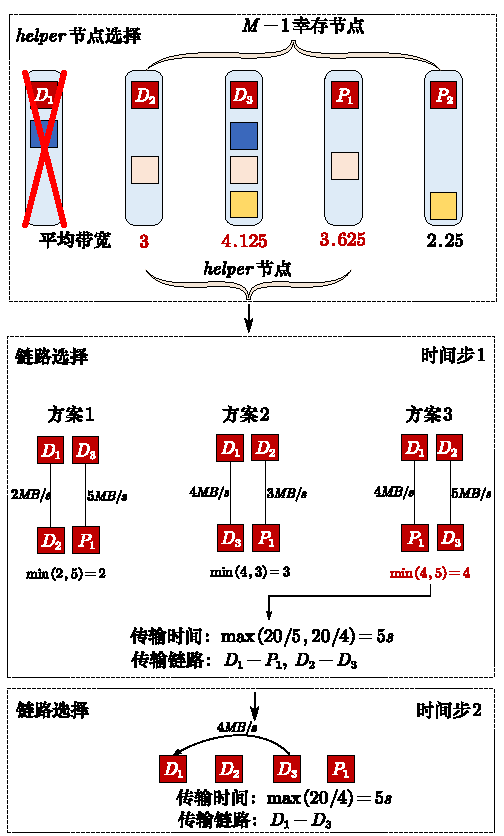
\includegraphics [scale=0.9]{figures/3.4.pdf}
	\caption{$helper$节点选择和链路选择过程图}
	\label{fig:3.4}
\end{figure}



在这个单节点修复的多级传输问题中,需要确定三个基本要素,即$helper$节点,链路选择和传输方向确定。在图~\ref{fig:3.3}中,
故障节点$N_f$中有块$D_1$,其中块的大小为$20MB$。当$D_1$丢失时,平均带宽最大的$k(k=3)$个正常节点为$D_3,P_1,D_2$,故$helper$
节点确定。在时间步1中,通过排列组合有三种修复方案,其中第三个方案的最低的链路在三个方案的最低中最大,因此时间步1的链路选择方案确定,
即$P_1\rightarrow D_1,D_2\rightarrow D_3$,其中方向分别是因为$D_1$为丢失的块和$D_3$的平均带宽大于$D_2$。
若选择了$D_3\rightarrow D_2$,那么在低链路带宽就会留到时间步2,相较而言造成的影响更大。当故障节点接收到块之后,
就可以通过解码参数来计算丢失的$D_1$,也就是$D_1=xD_2+yD_3+zP_1$。虽然在传递过程中,已经
通过绕过低链路和提高并行速度的方式来进行,但是带宽瓶颈的问题依然存在,并没有达到实时带宽的最优。
\begin{table}[tb!]
	% \setlength{\tabcolsep}{2.9pt}
	\centering
	\caption{7个节点测量带宽(MB/s)}
	% \begin{tabularx}{\textwidth}{lccccccc}
        % \resizebox{\textwidth}{!}{
	\begin{tabular}{ccccccccc}
		\toprule
		\textsc{带宽}                       & \textsc{$D_1$}    & \textsc{$D_2$}    & \textsc{$D_3$}    & \textsc{$P_1$}   & \textsc{$P_2$}      & \textsc{$I_1$}   & \textsc{$I_2$}      \\[1pt]
		\midrule
		\\[-15pt]
		\textsc{$D_1$}                      & *              & 2              & 4           & 4       & 2       & 8      & 4         \\
		\textsc{$D_2$}                      & 2              & *              & 5           & 3       & 2       & 10      & 5        \\
		\textsc{$D_3$}                      & 4              & 5              & *           & 5       & 2.5     & 10      & 5        \\
		\textsc{$P_1$}                      & 4              & 3              & 5           & *       & 2.5     & 10      & 5        \\
		% \multicolumn{14}{c}{using raw text}                                                                                                                                                                                                                                                                                                                                                                                                                              \\[1pt]
		\textsc{$P_2$}                      & 2              & 2              & 2.5         & 2.5     & *       & 5      & 8         \\
		\textsc{$I_1$}                      & 8              & 10             & 10          & 10      & 5       & *      & 5         \\
		\textsc{$I_2$}                      & 4              & 5              & 5           & 5       & 8       & 5      & *         \\
		% \hline
		% \\[-15pt]
		% \textsc{Loc}                      & 90.57          & 91.10          & 91.85                            & 81.68                           & 86.54                           & 90.47                            & 88.40                           & 91.53                            & 88.18                            & 90.65                           & 86.31                            & 92.91                            & 89.19                            \\
		% $\textsc{Loc}^{\textsc{mst}}$     & 90.56          & 91.03          & 91.98                            & 81.59                           & 86.83                           & 90.64                            & 88.23                           & 91.67                            & 88.20                            & 90.63                           & 86.51                            & 93.03                            & 89.23                            \\
		% \textsc{Crf}                      & 90.52          & \textbf{91.19} & 92.02                            & 81.43                           & 86.88\rlap{$^\dagger$}          & 90.76\rlap{$^\dagger$}           & 88.75                           & 91.76                            & 88.08                            & \textbf{90.79}                  & 86.54                            & 93.16\rlap{$^\ddagger$}          & 89.32\rlap{$^\ddagger$}          \\
		% \textsc{Crf2o}                    & \textbf{90.76} & 91.12          & \textbf{92.15}\rlap{$^\ddagger$} & \textbf{81.94}                  & \textbf{86.93}\rlap{$^\dagger$} & \textbf{90.81}\rlap{$^\ddagger$} & \textbf{88.83}\rlap{$^\dagger$} & \textbf{92.34}\rlap{$^\ddagger$} & \textbf{88.21}\rlap{$^\dagger$}  & 90.78                           & \textbf{86.62}                   & \textbf{93.22}\rlap{$^\ddagger$} & \textbf{89.48}\rlap{$^\ddagger$} \\
		% \textsc{Crf2o}                    & 90.15          & 91.39          & 91.10                            & 83.39                           & 88.52                           & 90.84                            & 88.59                           & 92.49                            & 88.37                            & 92.82                           & 84.89                            & 93.11                            & 89.85                            \\
		% \textsc{Crf2o}                    & \textbf{91.32} & \textbf{92.57} & \textbf{92.66}                   & \textbf{84.56}                  & \textbf{88.98}                  & \textbf{91.88}                   & \textbf{89.83}                  & \textbf{92.94}                   & \textbf{89.85}                   & \textbf{93.26}                  & \textbf{87.39}                   & \textbf{93.86}                   & \textbf{90.76}                   \\
		\bottomrule
	\end{tabular}
        % }
	\label{table:3-1}
\end{table}


通过加入空闲节点(idle nodes)进行数据中继的方式可以对传输问题进一步优化。如图~\ref{fig:3.5}所示,空闲节点中不包含
同一条带中的数据块或者包含其他条带的数据块,在修复过程中处于空闲状态,没有进行其他修复任务的传输。可以看出通过空闲节点的中继,
有效减少了传输时间,原本的$P_1\rightarrow D_1$需要$5s$,然而通过$I_1$进行中继后的$P_1\rightarrow I_1 \rightarrow D_1$
只需要$4s$。为了简化问题,假设每个空闲节点同时只能执行一种转发任务,在多级转发过程中,需要源头节点和目标节点以及中继节点集合,问题
的目标是找到一条消耗时间最短的链路路径,例如图~\ref{fig:3.5}中的$P_1,D_1$和$I_1,I_2$组成的集合,且这样的组合路径可以用树来进行表示。
$P_1$节点则为树根,$D_1$为叶子节点,空闲节点的集合则可以表示为非叶节点,其中任何一条从树根到叶子节点的路径则为一条转发链路,假设
共有$x$个非叶节点,则一共有$C_{x}^{1}+C_{x}^{2}+\cdots+C_{x}^{x}$种转发链路的可能。当$x$变得很大的时候,寻找路径的算法复杂度将会
非常高。针对此问题\citet{zhou2022bandwidth}提出了可以绕过低带宽的链路,
更快地将数据传输到目标节点.故而提出了带宽感知的多级调度算法SMFRepair
(single-node multi-level forwarding repair algorithm)。

\begin{figure}[htbp]
	\centering
	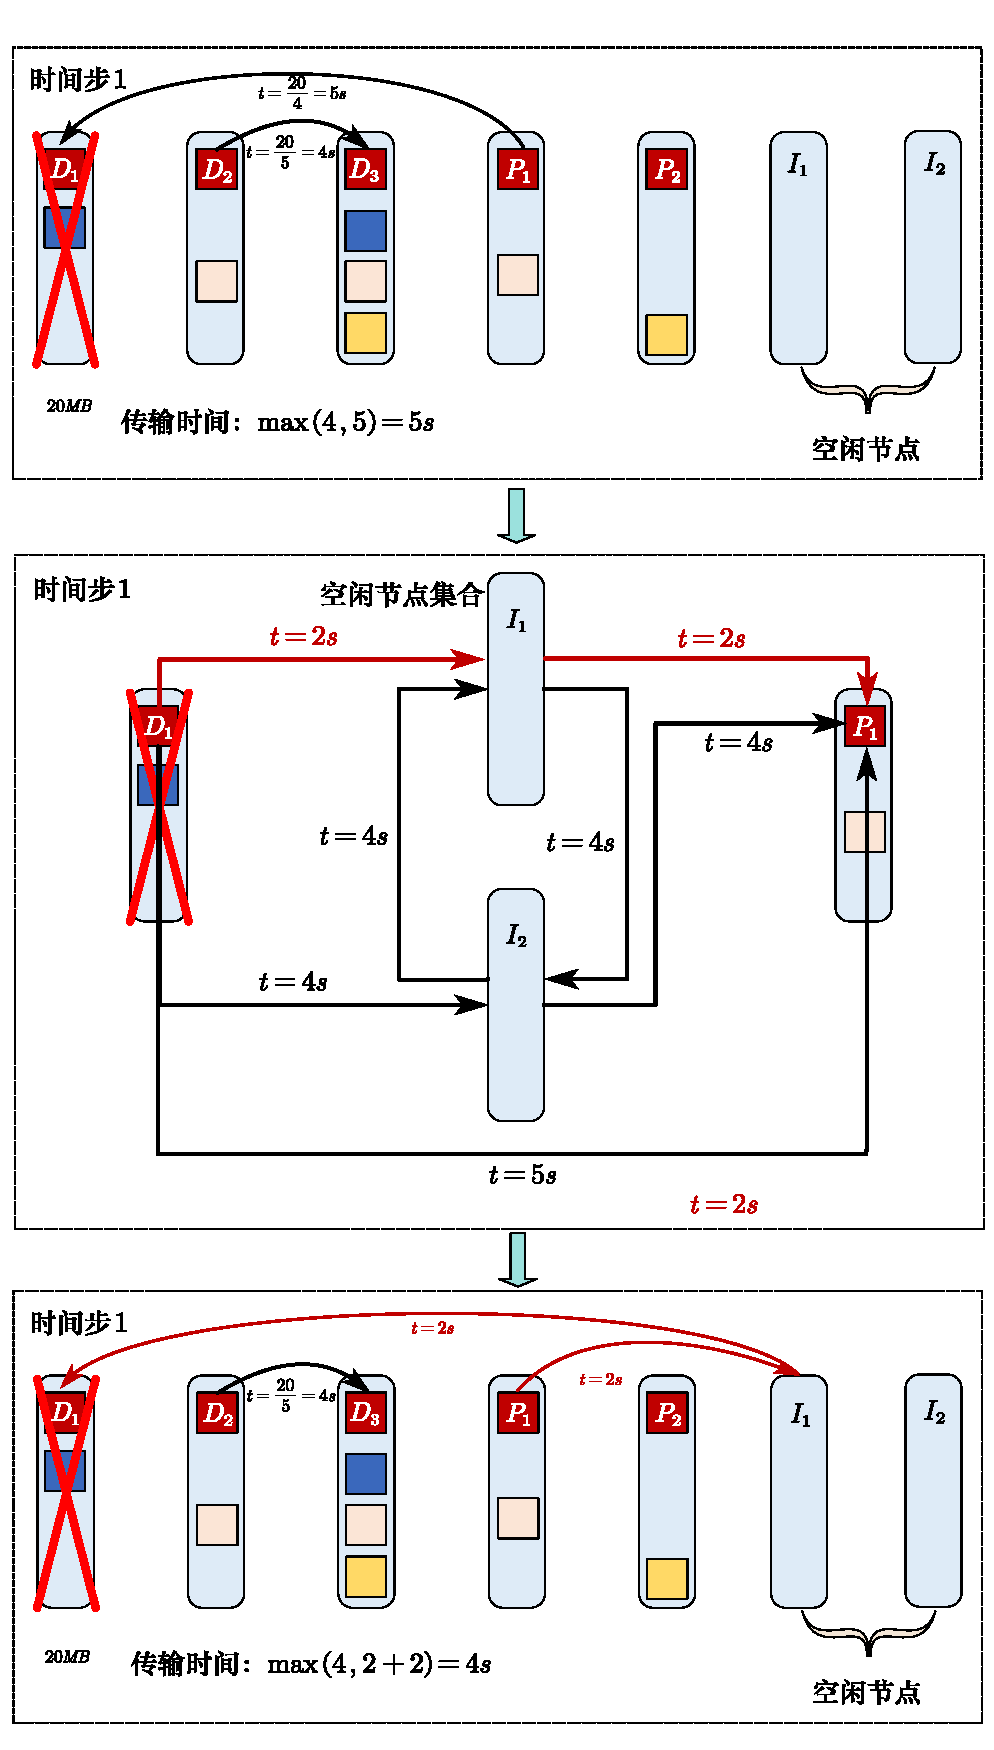
\includegraphics [scale=0.5]{figures/3.5.pdf}
	\caption{结合空闲节点的链路传输优化过程图}
	\label{fig:3.5}
\end{figure}

SMFRepair不仅可以运用在重建技术上,本文在该算法的基础上将其运用到了迁移技术上并进行了改善。
该算法基于PPR技术,改善了PPR容易受到异构环境中低链路带宽的影响,提高每轮修复的效率,从而在整个修复过程中达到最优。
图~\ref{fig:3.6}显示了具体的优化过程,假设每个节点只能协助转发一次(避免性能瓶颈和逆向转发),
整个转发过程包括两个节点和一个集合。在重建任务中两个节点是源节点$N_1$和目标节点$N_2$,
闲置节点则是含有相同条带的其他块的节点的集合,称之为转发中间节点集。
在迁移任务中,两个节点的源节点为STF节点,目标节点为不含有相同条带的其他块的节点,例如$N_2$,
闲置节点则为所有可用节点,定义为迁移任务的中间集。
优化的目标就是找到一条从源节点出发,经过中间集,到达目标节点的最短路径。
其中,从源节点到中间集以及中间集到目标节点的链接是单向的,中间集中的每个节点都是双向互通的,但每个节点只能通过一次。

\begin{figure}[htbp]
	\centering
	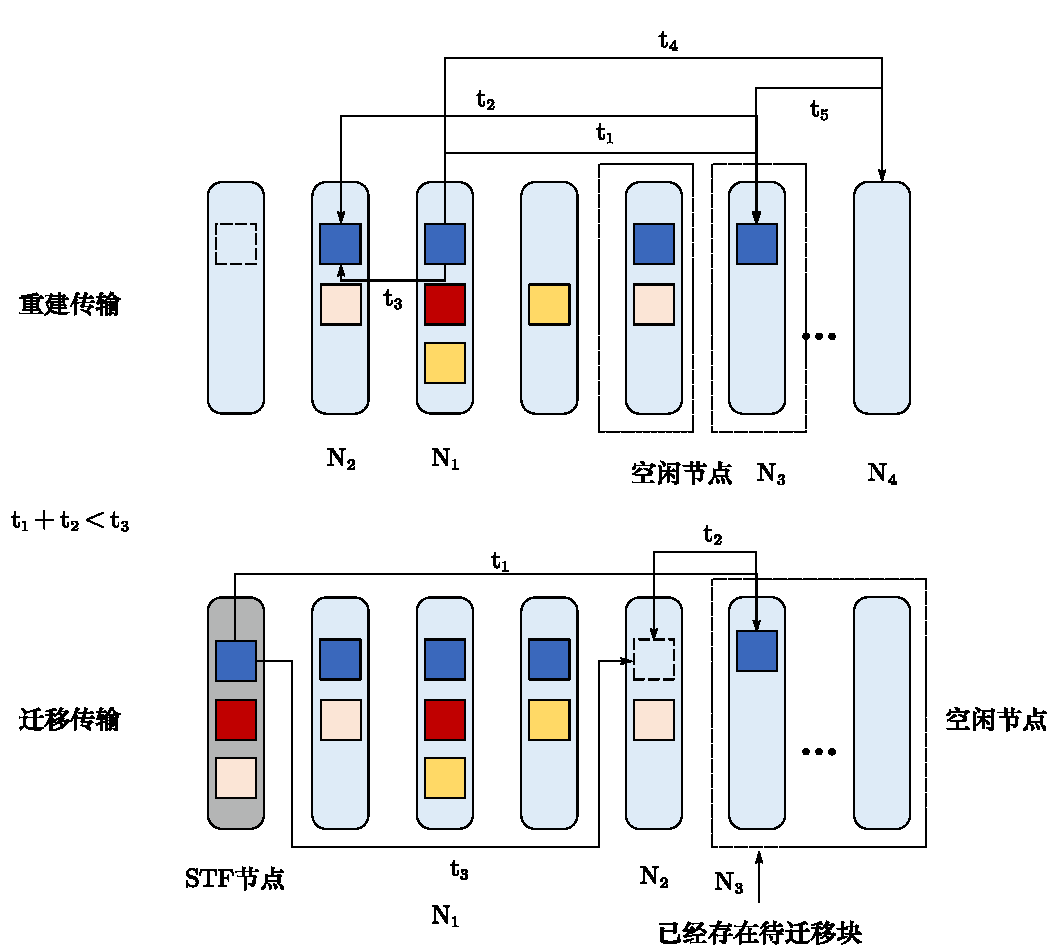
\includegraphics [scale=0.5]{figures/3.6.pdf}
	\caption{重建与迁移的中继传输}
	\label{fig:3.6}
\end{figure}

对于纠删码结构为$RS(n,k)$的分布式存储集群来说,当某个节点失效,相应的数据块不可访问时,对于重建任务而言,一般情况下需要在剩下
的$M-1$个节点中检索$k$个从属于同一个条带的数据进行数据修复,通常会有两种情况(结合图~\ref{fig:3.6}进行阐述):

\begin{enumerate}
	\item 从节点$N_1$检索到一个块,从其传输到节点
	      $N_3$,同时节点$N_3$也含有相应的从属于同一个条带的数据块,此时节点$N_3$含有两个可以传输的同一个条带的数据块,将其传输到节点
	      $N_2$进行修复,总共花费的时间为$t_1+t_2$,小于直接从节点$N_1$传输数据到节点$N_2$所花费的时间$t_3$;
	\item 从节点$N_1$
	      检索到一个块,从其传输到节点$N_4$,同时节点$N_4$并不含有相应的从属于同一个条带的数据块,可能含有其他数据块或者没有,然后从节点
	      $N_4$将数据块转发到节点$N_3$,之后的流程与情况(1)相同,而花费的总时间为$t_4+t_5+t_2<t_1+t_2$,即$t_4+t_5<t_1$,
	      在这种情况下,在两个均含有相同条带的数据块的节点传输数据的速度慢于先将数据块传输到空节点(或者含有其他条带的数据块)
	      再转发到另一个含有相同条带的数据块的节点的速度。
	      对于迁移任务而言,一般只有一种情况需要考虑:当有STF节点产生时,则需要将数据块迁移到不存放该条带下数据块的节点$N_2$,
	      首先将其传输到已经含有相同条带下数据块的节点$N_3$,然后再从节点$N_3$将数据块转发设计的目标节点$N_2$,所消耗的总时间为
	      $t_1+t_2$,且小于直接将数据块从STF节点传输到目标节点$N_2$的时间$t_3$。
\end{enumerate}

针对上述情况的特点,节点传输过程主要通过类似最短路的机制来减少整个修复所消耗的时间。
可以通过计算最短路径的Dijkstra算法(O(NLogN))求得最优的转发修复方案。如图~\ref{fig:3.7}所示,
主要是通过建立一个图结构来描述问题,图的源节点为$N_1$或$N_2$,
对于重建任务需要从含有该块的节点出发,则源节点为$N_1$,
对于迁移任务需要从STF节点出发,经过若干次跳跃,最终节点一定是未包含该条带的节点,所以源节点是$N_2$。
从源节点开始,逐个计算每条路径消耗的权重时间,可以通过剪枝来加快算法的运行,
即对于某些情况下,路径消耗一定是大于当前已经遍历的情况,则在算法运行中不纳入考虑。
\begin{figure}[htbp]
	\centering
	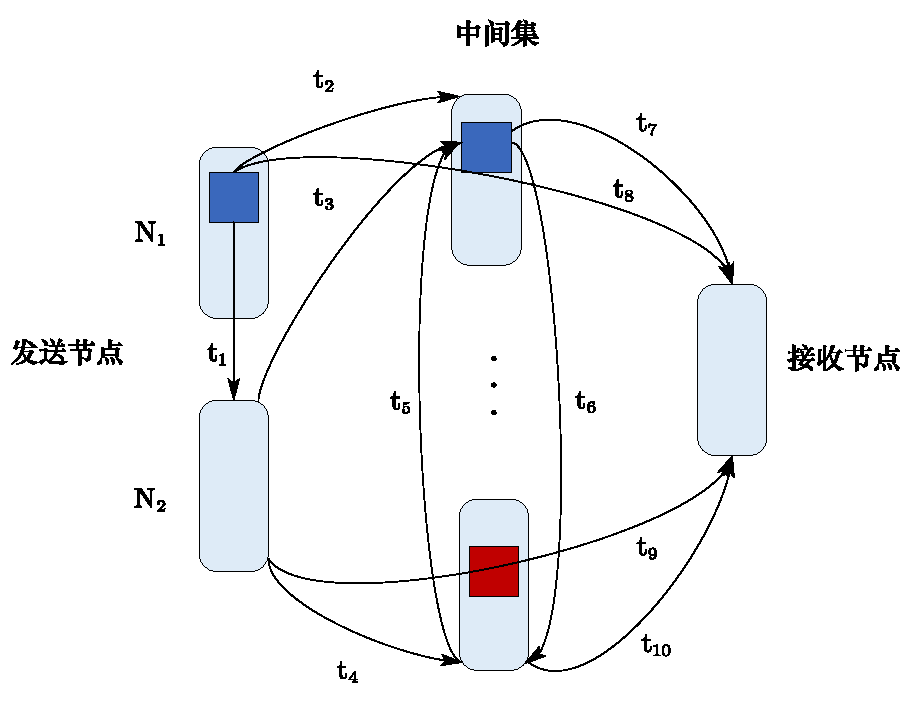
\includegraphics [scale=0.5]{figures/3.7.pdf}
	\caption{节点中继的流程}
	\label{fig:3.7}
\end{figure}


因此本文针对迁移与重建问题的调度特性,设计了改进的SMFRepair算法(IBA,Improved SMFRepair Algorithm)算法。
原算法在修复过程中总是构建当前带宽的全局最优路径,使用的是树的搜索算法,
由于本文需要解决的是重建与迁移交融的修复任务,所以在寻找最优路径的过程中使用的是Dijkstra算法。
IBA在每一轮修复中首先判断该任务是迁移还是重建,根据输入参数type进行确认,紧接着采用局部最优修复(第4$\sim$11行),
在此过程中链路带宽不断发生变化,从而实现最优化。详细算法如算法~\ref{alg:3-2}所示,具体效果将在随后的实验中展现。


\begin{algorithm}[htpb]
	\begin{algorithmic}[1]
		% \newlength{\commentindent}
		\setlength{\commentindent}{.3\textwidth}
		\setlength{\algorithmicindent}{1.5em}
		\renewcommand{\algorithmiccomment}[1]{\unskip\hfill\makebox[\commentindent][l]{$\rhd$~#1}\par}
		\LetLtxMacro{\oldalgorithmic}{\algorithmic}
		\renewcommand{\algorithmic}[1][0]{
			\oldalgorithmic[#1]
			\renewcommand{\ALC@com}[1]{
				\IFnum\pdfstrcmp{##1}{default}=0\ELSE\algorithmiccomment{##1}\fi}%
		}
		\REQUIRE{$\textbf{w}={(w_1,w_2,...)}$,type}
		\ENSURE{$\textbf{NewW}$}
		\STATE $\textbf{NewW} = \textbf{w}$;
		\WHILE {true}
		\STATE R = FindMaxTimeRoad($\textbf{NewW}$);
		\IF {type == 1}
		\STATE S = FindNodeWithoutChunk($\textbf{NewW}$);
		\STATE D = R.Destination;
		\ELSE
		\STATE S, D = R.Source, R.Destination;
		\ENDIF
		\STATE RIdle = GetIdleNode(R);
		\STATE NewR = DijkstraMinTimeRoad(S, D, RIdle);
		\STATE Update($\textbf{NewW}$, NewR);
		\IF {FindMaxTimeRoad($\textbf{NewW}$) == R}
		\STATE break;
		\ENDIF
		\ENDWHILE
		\STATE $\textbf{return}$ $\textbf{NewW}$;
	\end{algorithmic}
	\caption{Improved SMFRepair Algorithm}
	\label{alg:3-2}
\end{algorithm}

\section{实验结果与分析}
我们对SMSRS和ISA算法进行了仿真实验,以评估其在大规模存储集群中的性能。
基于SimEDC\cite{zhang2019simedc}我们为算法原型为设计了一个仿真平台。
SimEDC是一个用于模拟离散事件程序集,
其主要功能是用来特征量化基于纠删码构建的数据中心的可靠性。
它旨在通过接收多种影响因子的输入,包括数据中心拓扑,纠删码(例如,经典的Reed-Solomon码,以及最近提出的LRC和DRC),
数据的冗余放置(即单节点单块数据和单节点多块数据),以及数学统计模型或系统历史运行数据的不同子系统的故障或者修复模式,
同时可以量化基于纠删码构建的数据中心的持久性和可靠性的量化指标。
此外,它可以采用重要性采样来加速整个仿真模拟的过程,从而能够对基于纠删码构建的数据中心的可靠性进行全面的仿真模拟分析。
在我们的仿真平台中,没有实现编码操作,因为主要是将本文算法原型与FastPR和SMFRepair进行性能比较。

\subsection{实验环境}
实验环境是在虚拟机中配置的Ubuntu 16.04 LTS系统,配置为3.70GHz Intel Core i5-9600K处理器,16GB内存,1 Gbit/s网络接口。
在该系统中通仿真平台搭建了分布式存储系统集群,集群包含100个节点,磁盘带宽上限$b_d=100MB/s$,网络带宽上限$b_n=1Gb/s$,3个空闲节点(只用于转发)。
我们用$RS(6,4)$,$RS(9,6)$\cite{ovsiannikov2013quantcast}(QFS采用的编码策略),
$RS(14,10)$\cite{muralidhar2014f4}(Facebook采用的编码策略),$RS(16,12)$\cite{huang2012erasure}(Azure采用的编码策略)四种
RS码进行对比实验。其中将块大小固定为$64MB$和$128$MB两种情况,并在存储集群中随机分布$1,000$个条带的块,测试结果采用运行50次以上的平均结果。




\subsection{修复与调度实验}

\begin{figure}[htbp]
	\centering
	\begin{subfigure}[t]{0.4\textwidth}
		\centering
		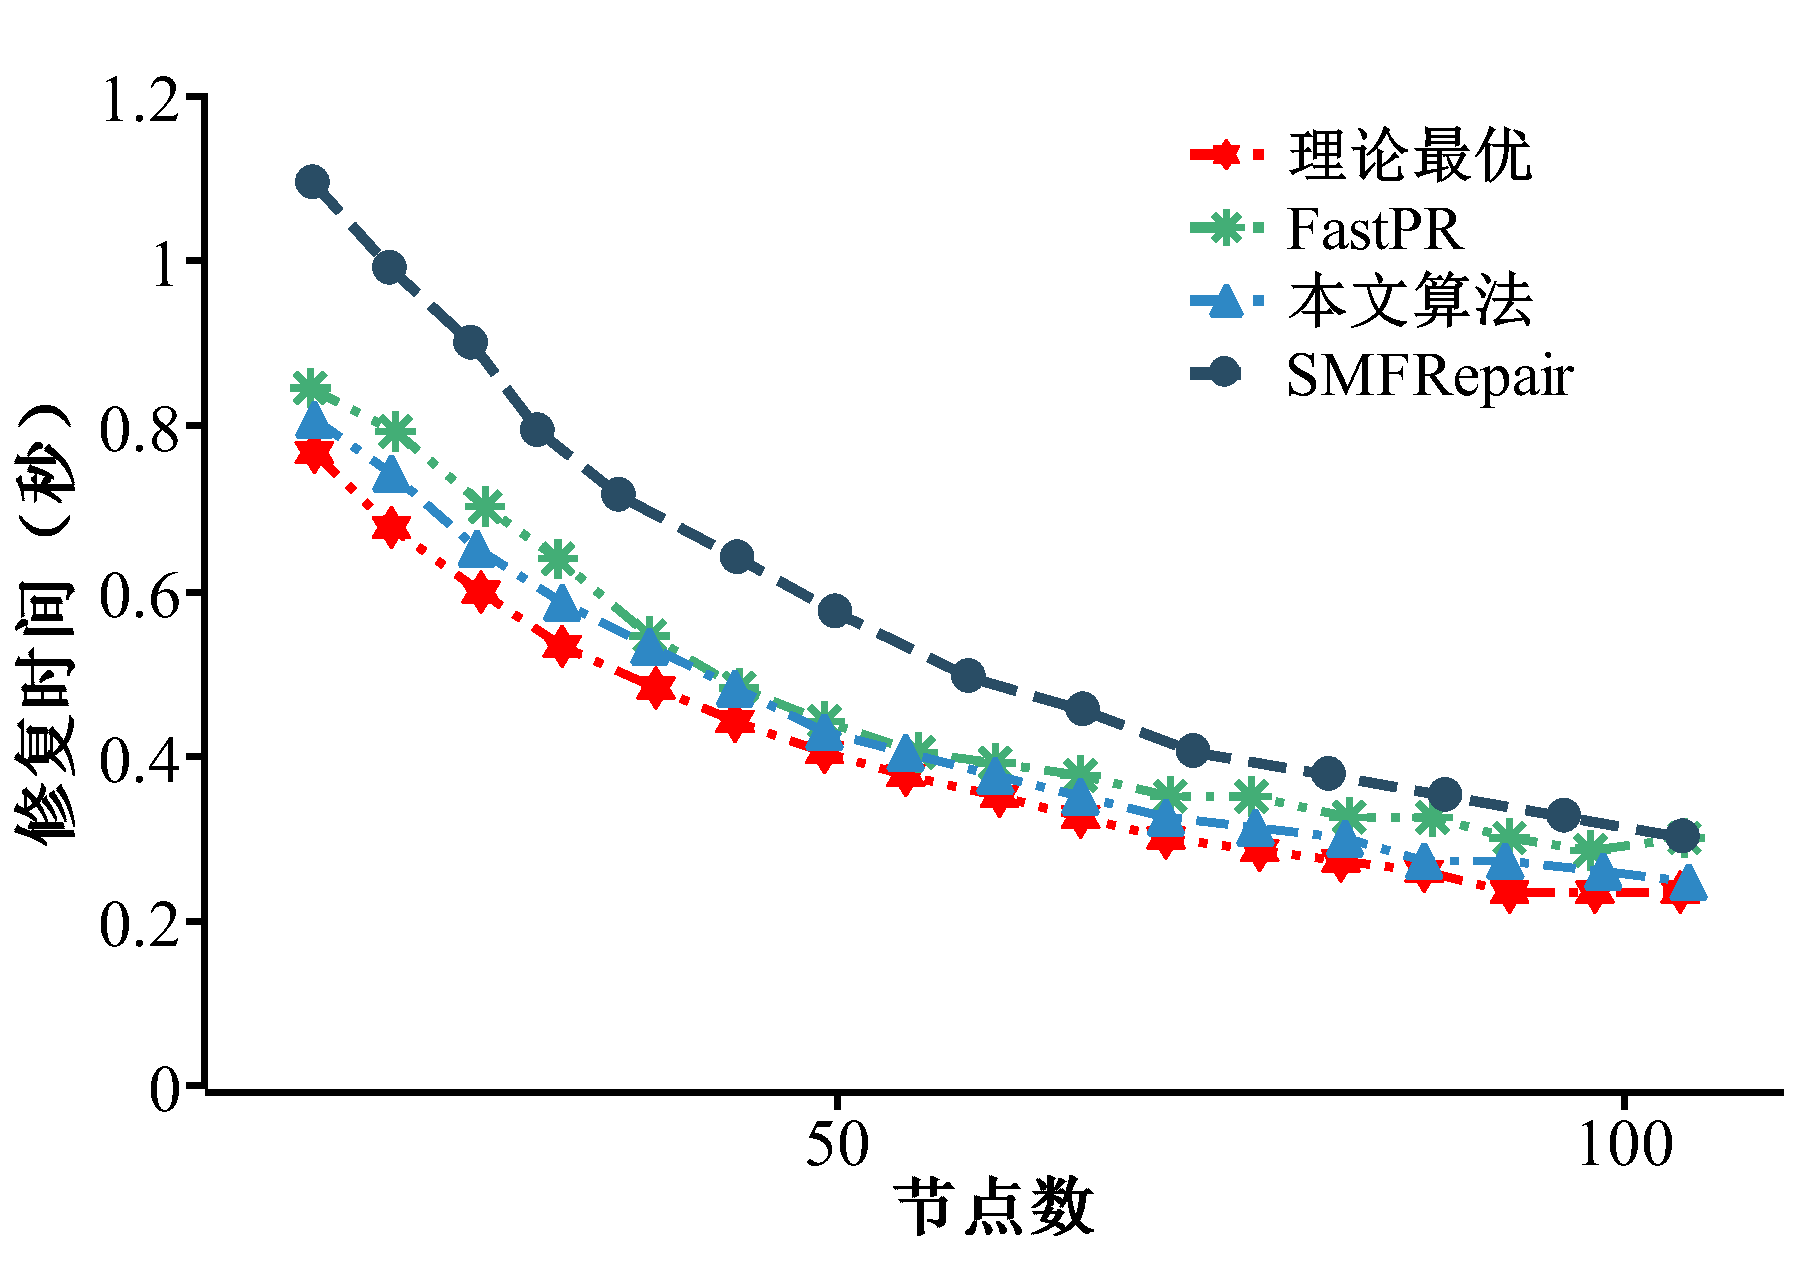
\includegraphics[width=1.0\linewidth]{figures/3-8.pdf}
		\caption{总节点数$M$值理论结果}
		\label{fig:3-8}
	\end{subfigure}
	\begin{subfigure}[t]{0.4\textwidth}
		\centering
		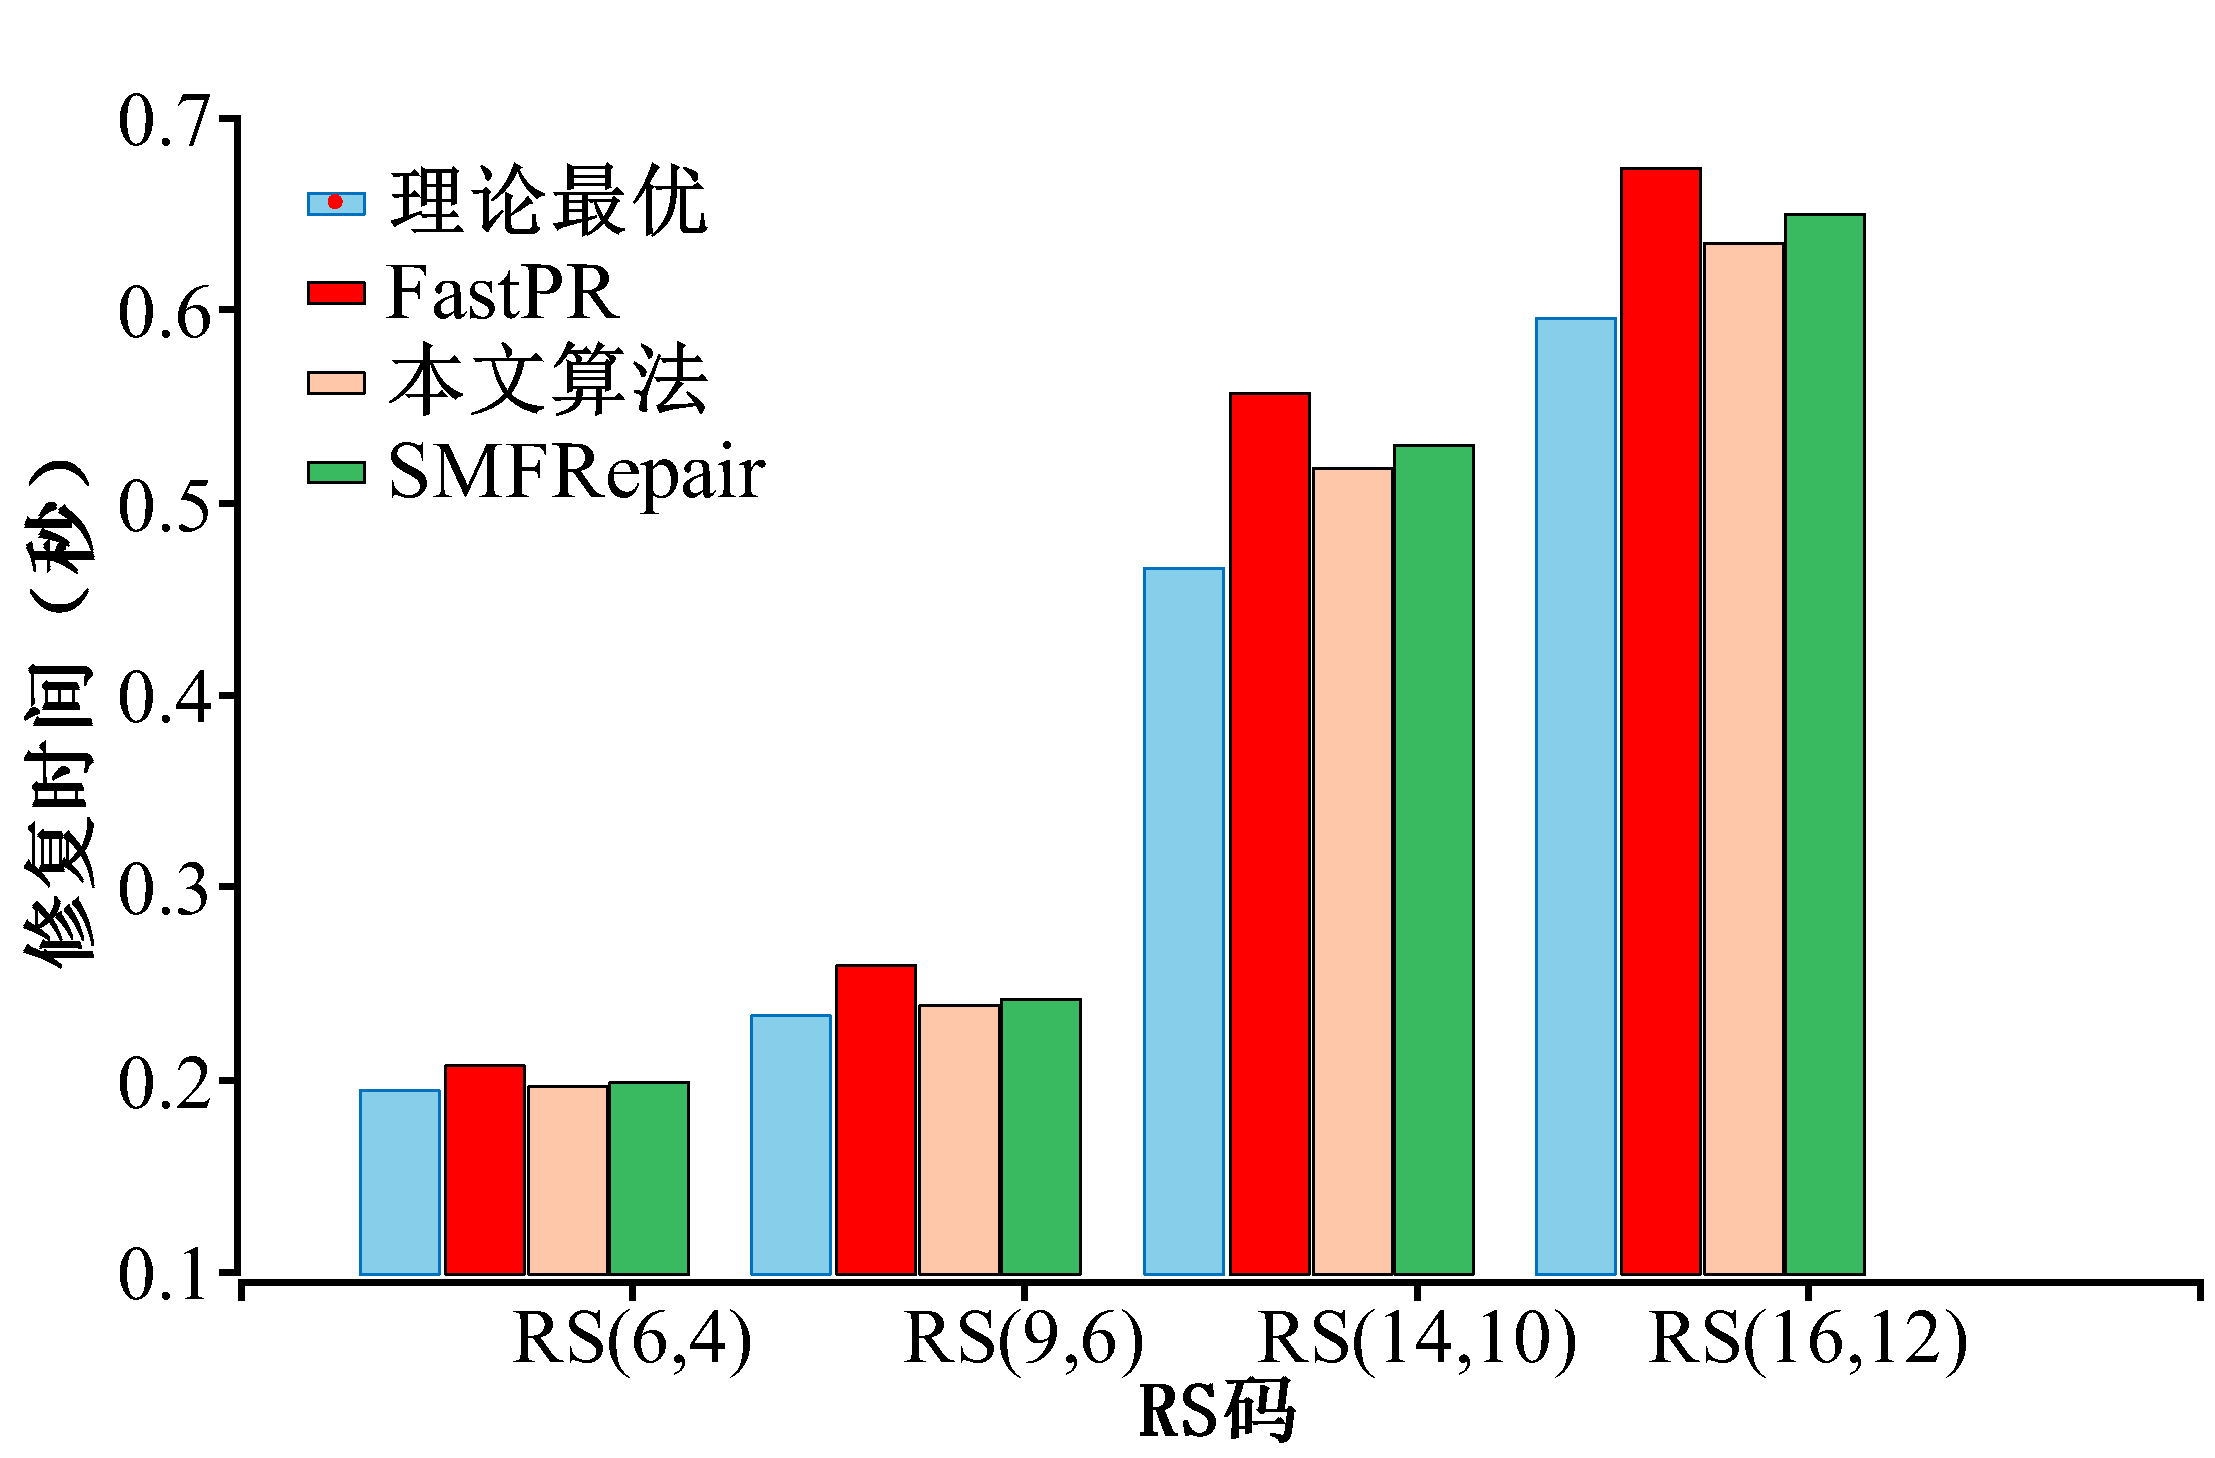
\includegraphics[width=1.1\linewidth]{figures/3-9.pdf}
		\caption{$RS(n,k)$配置理论结果}
		\label{fig:3-9}
	\end{subfigure}
	\begin{subfigure}[t]{0.4\textwidth}
		\centering
		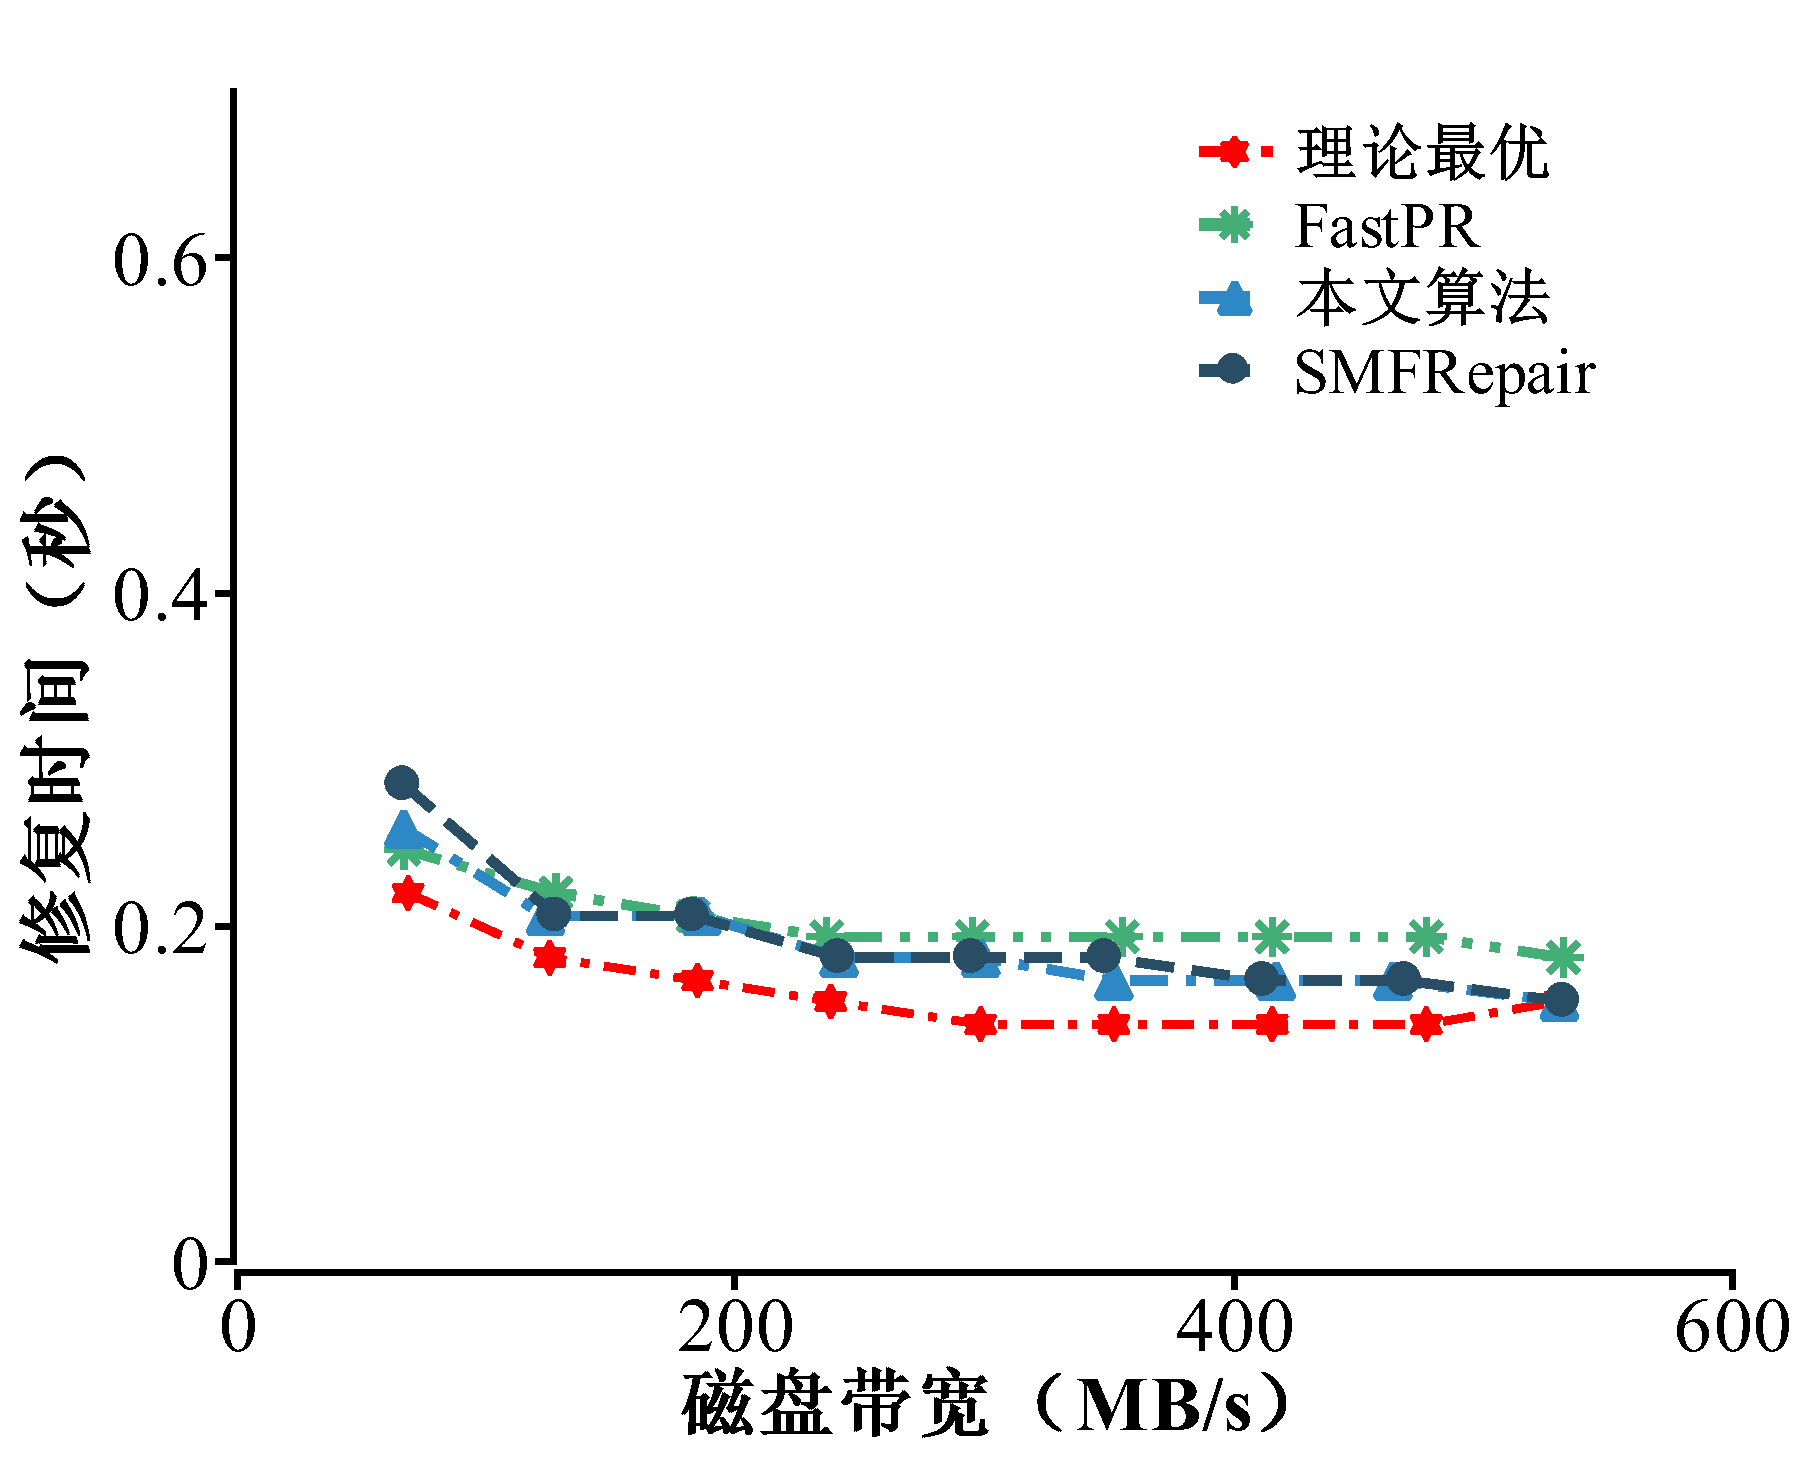
\includegraphics[width=1.1\linewidth]{figures/3-10.pdf}
		\caption{磁盘带宽$b_d$理论结果}
		\label{fig:3-10}
	\end{subfigure}
	\begin{subfigure}[t]{0.4\textwidth}
		\centering
		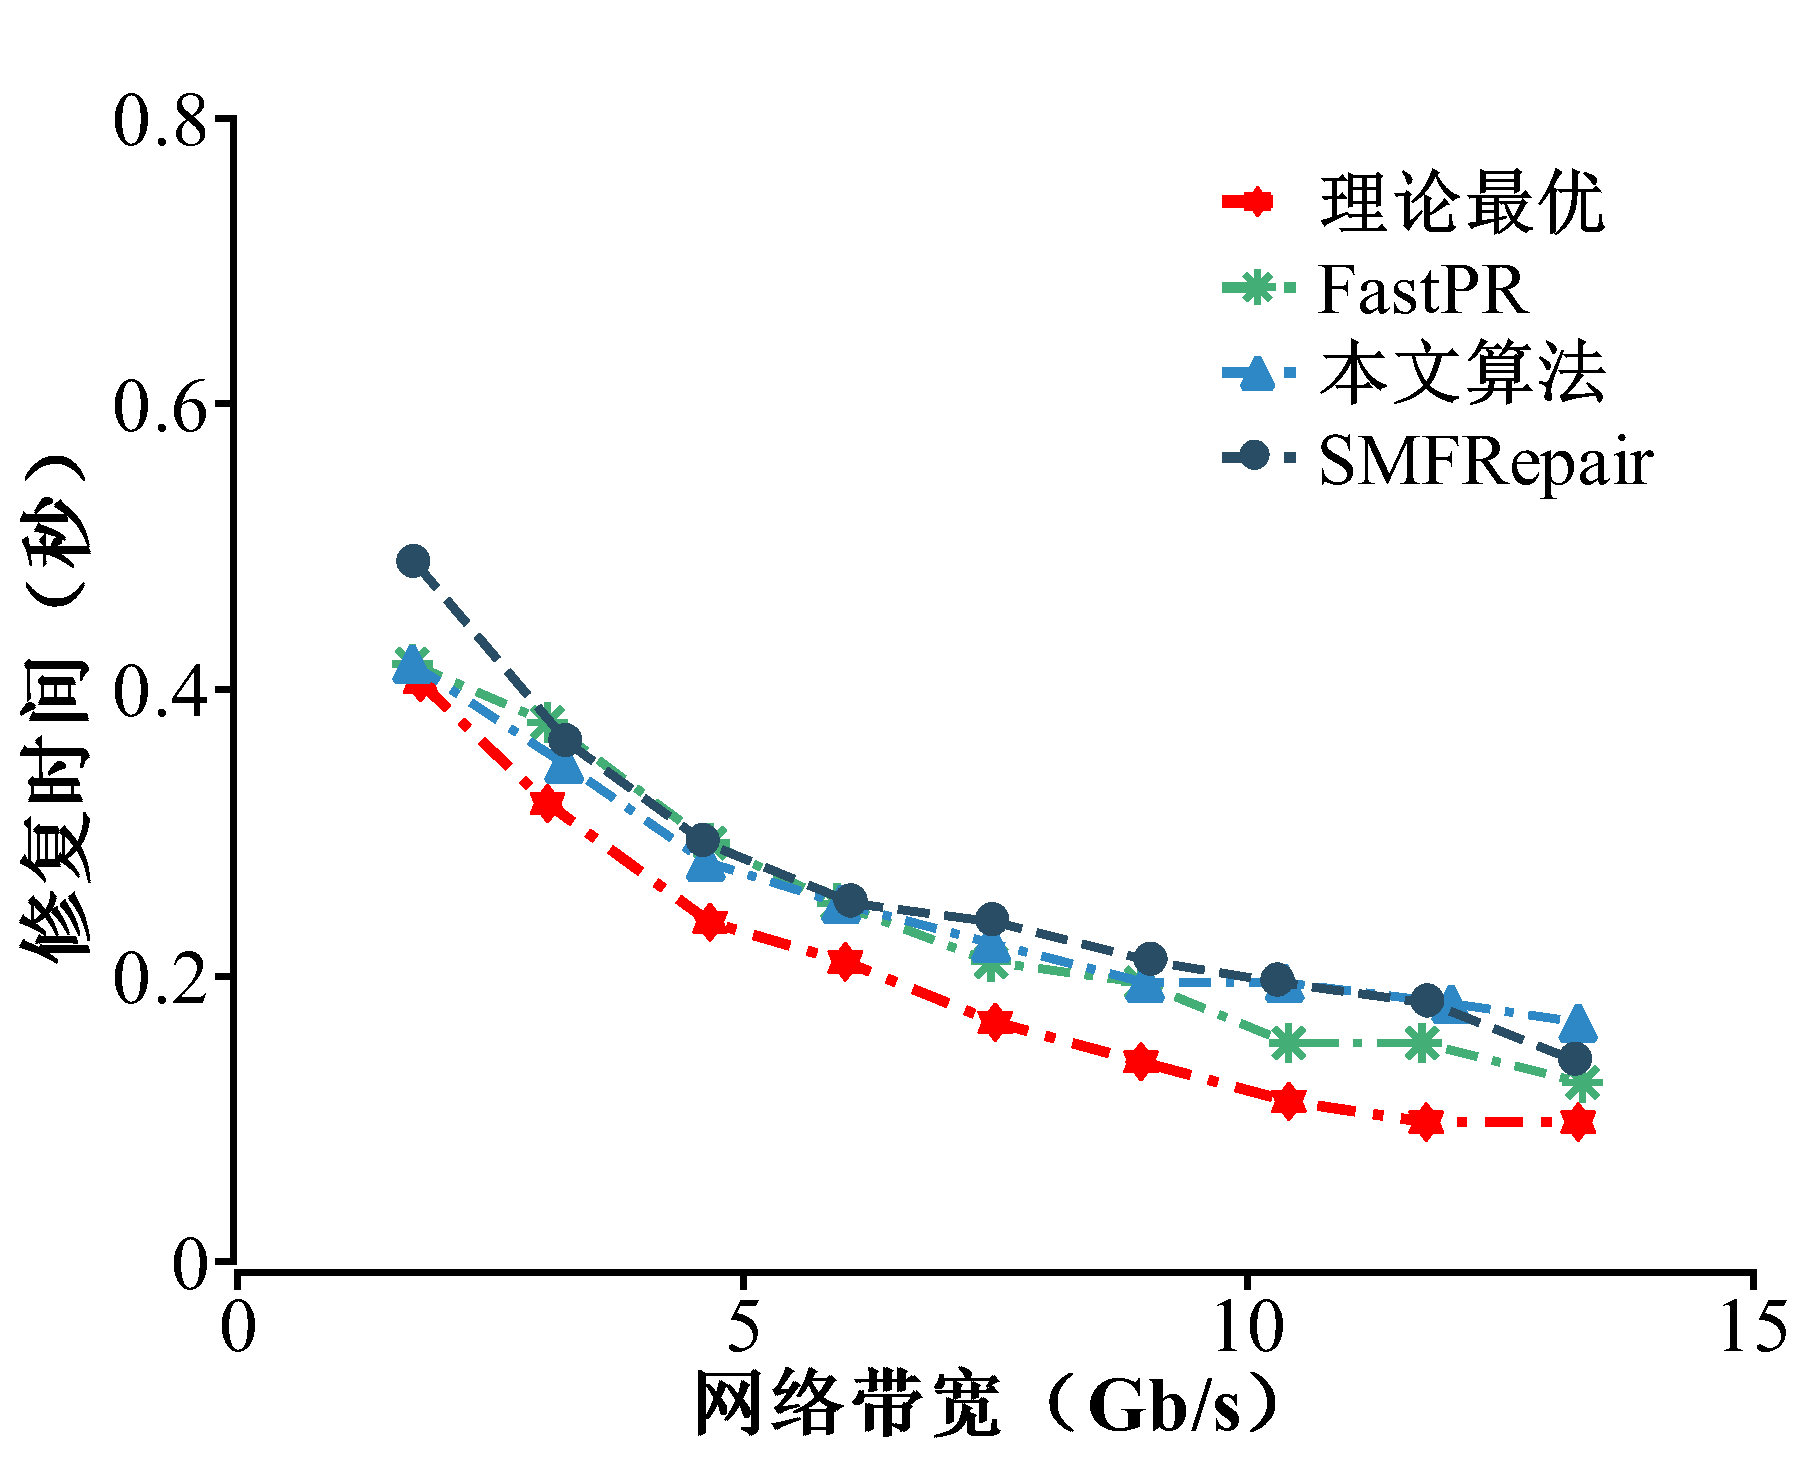
\includegraphics[width=1.1\linewidth]{figures/3-11.pdf}
		\caption{网络带宽$b_n$理论结果}
		\label{fig:3-11}
	\end{subfigure}
	\caption{预测修复与反应式修复建模对比}
	\label{fig:3-8-11}
\end{figure}


\subsection{条带数的影响}

\begin{figure}[htbp]
	\centering
	\begin{subfigure}[t]{0.4\textwidth}
		\centering
		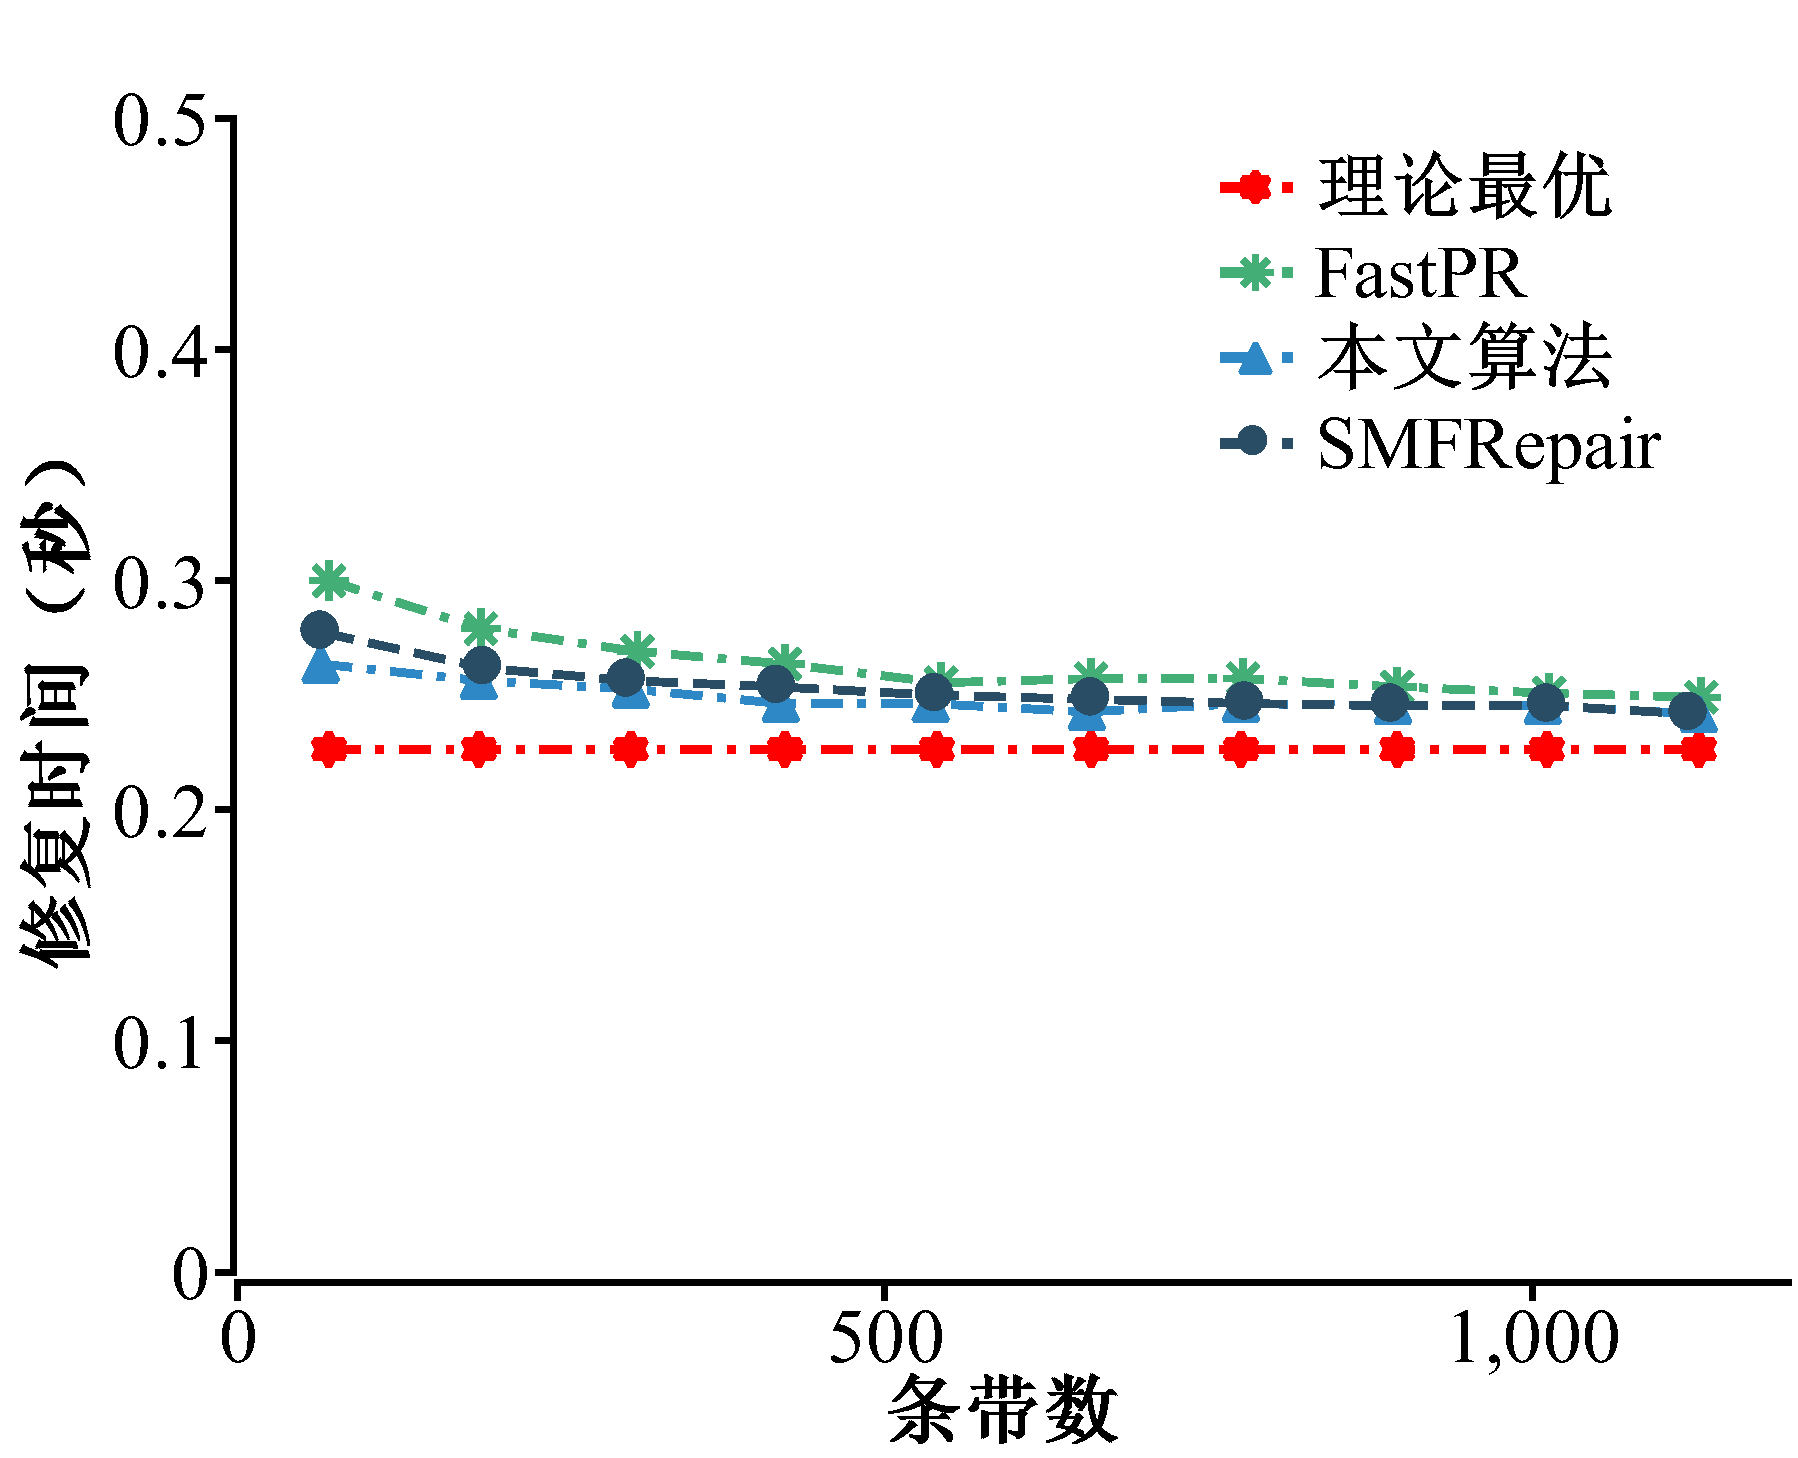
\includegraphics[width=1.0\linewidth]{figures/3-12.pdf}
		\caption{总节点数$M$值理论结果}
		\label{fig:3-12}
	\end{subfigure}
	\begin{subfigure}[t]{0.4\textwidth}
		\centering
		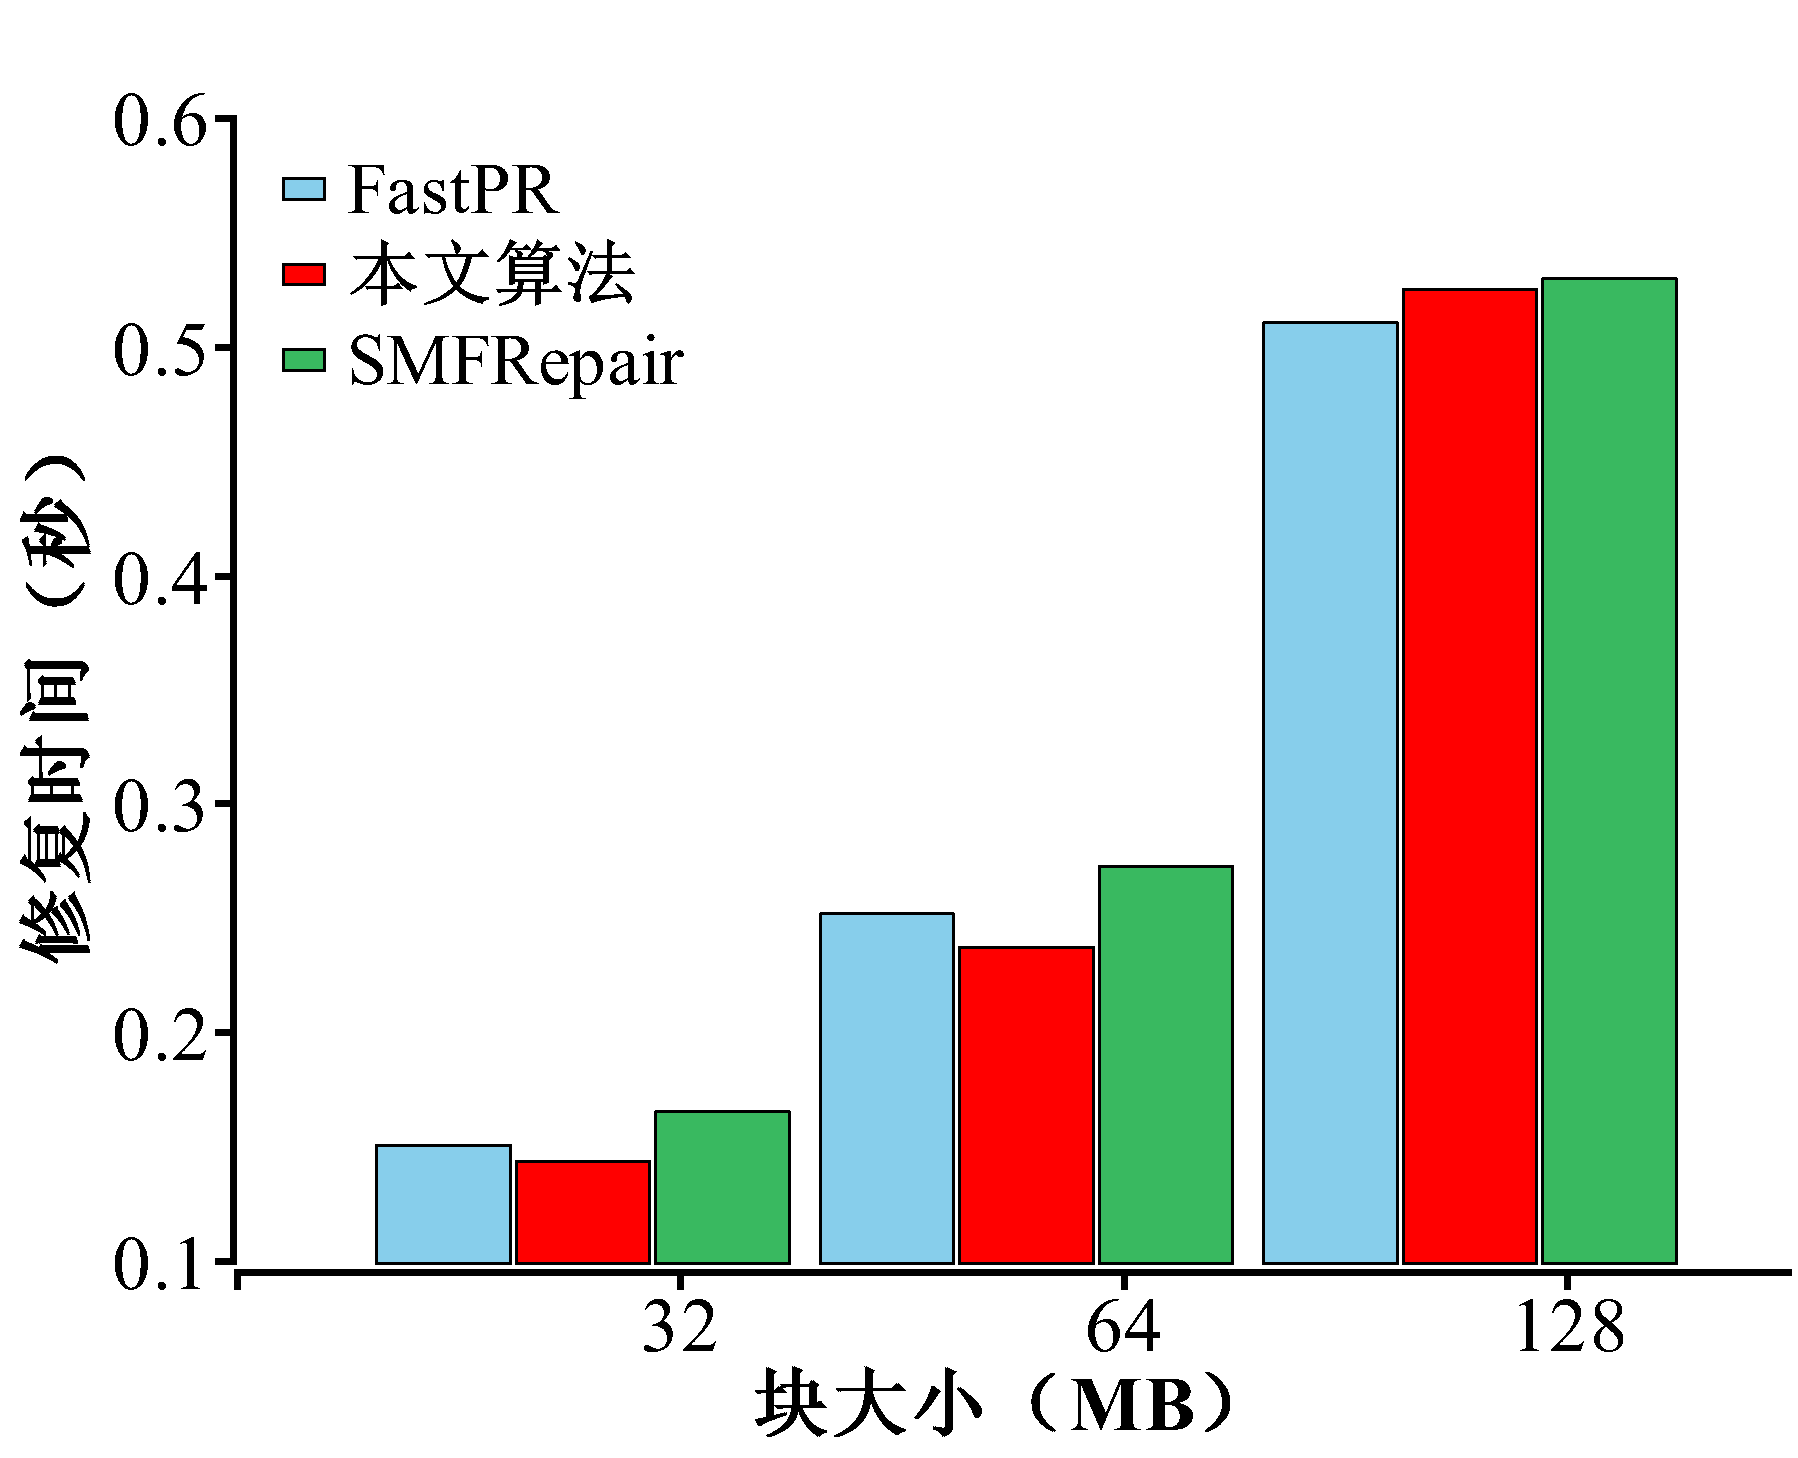
\includegraphics[width=1.1\linewidth]{figures/3-14.pdf}
		\caption{$RS(n,k)$配置理论结果}
		\label{fig:3-14}
	\end{subfigure}
	\caption{预测修复与反应式修复建模对比}
	\label{fig:3-12-14}
\end{figure}

\subsection{空闲节点数的影响}


\begin{figure}[htbp]
	\centering
	\begin{subfigure}[t]{0.4\textwidth}
		\centering
		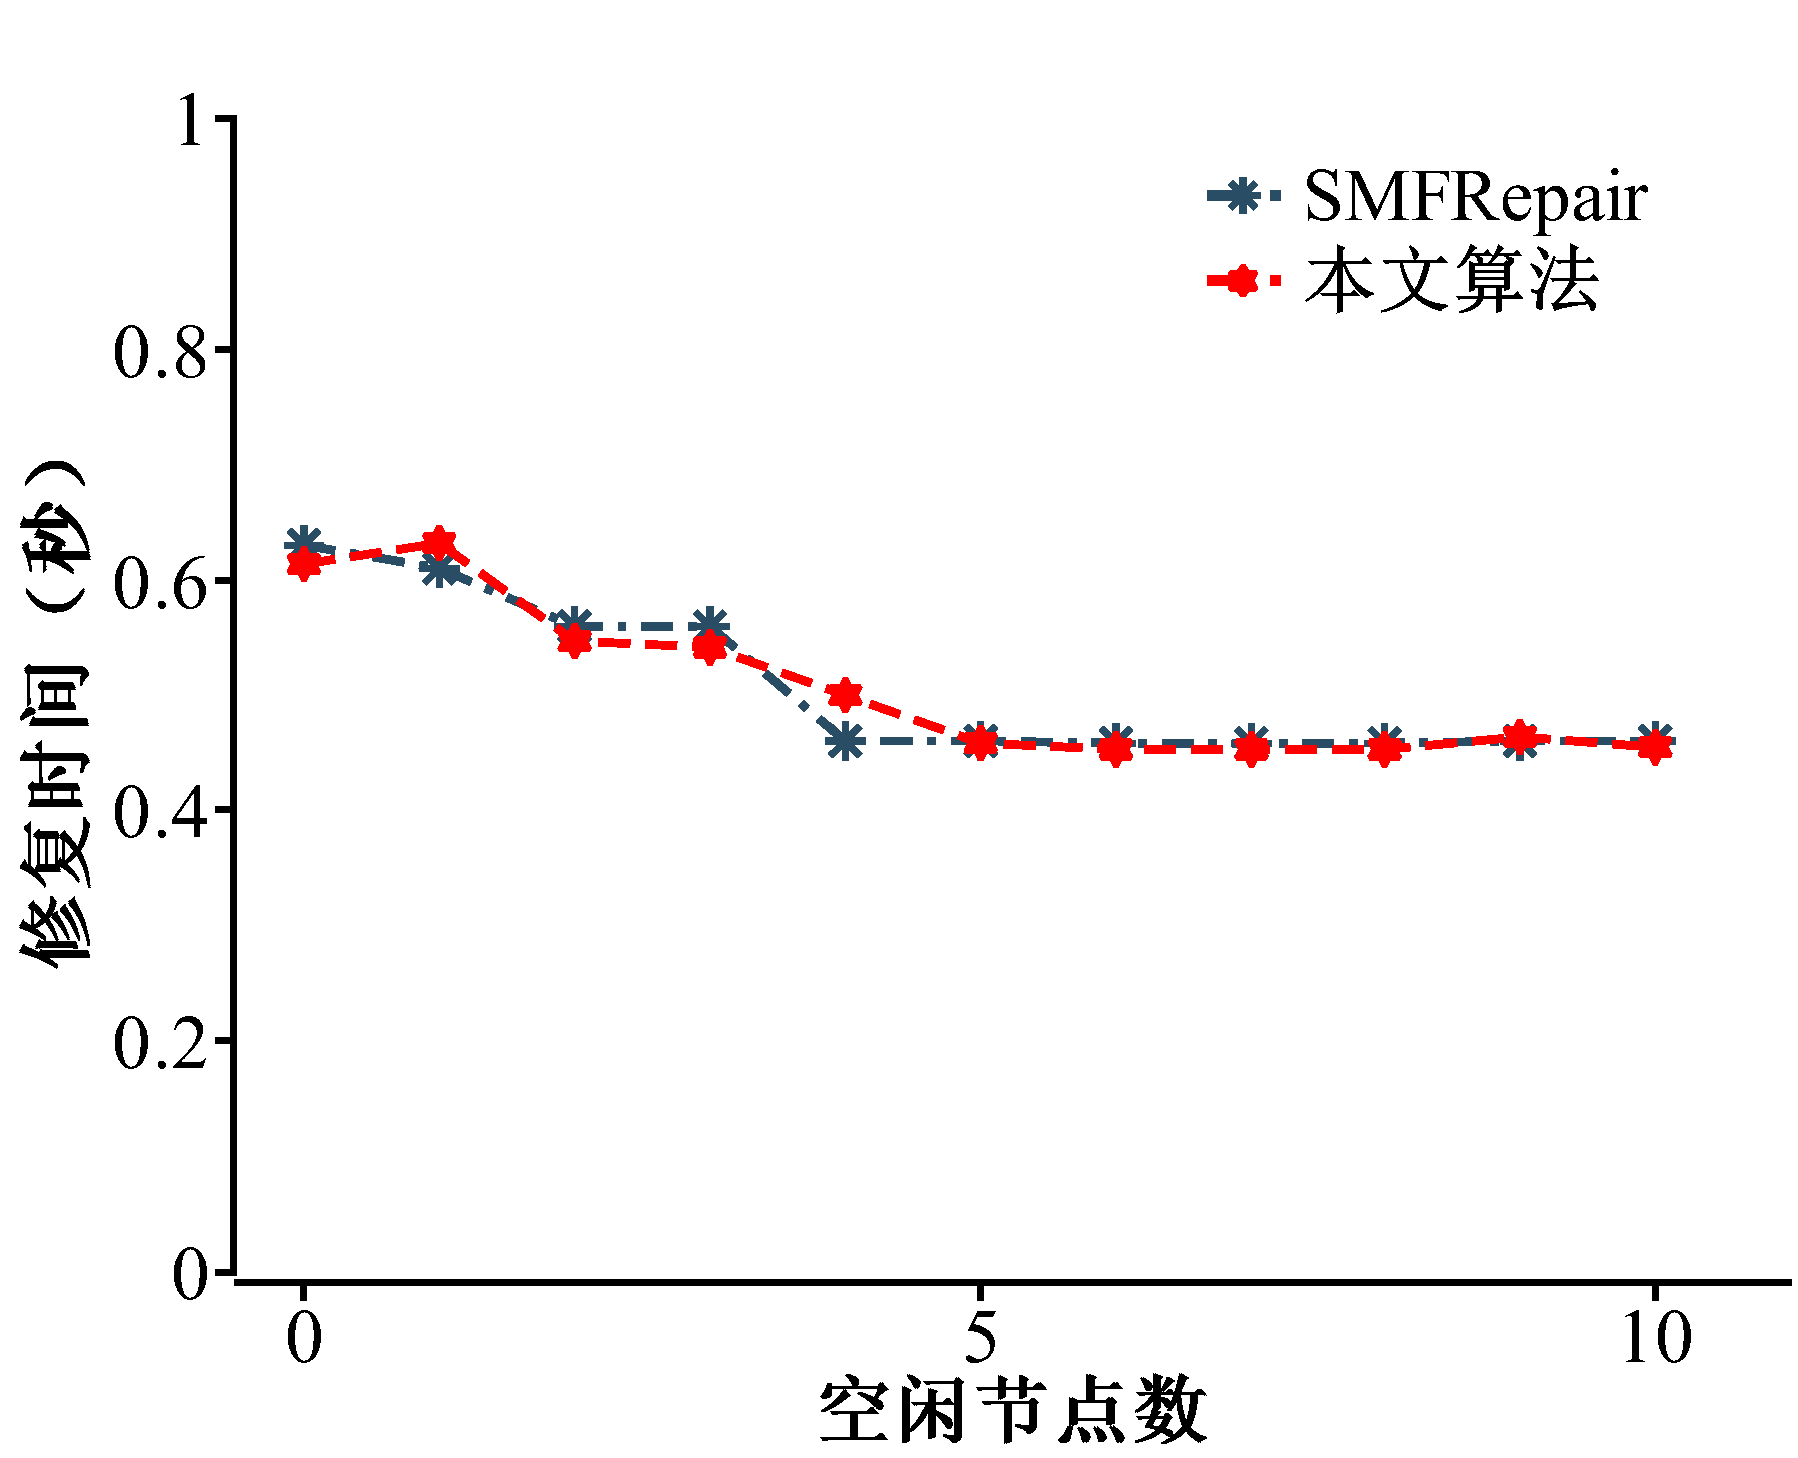
\includegraphics[width=1\linewidth]{figures/3-15.pdf}
		\caption{总节点数$M$值理论结果}
		\label{fig:3-15}
	\end{subfigure}
	\begin{subfigure}[t]{0.4\textwidth}
		\centering
		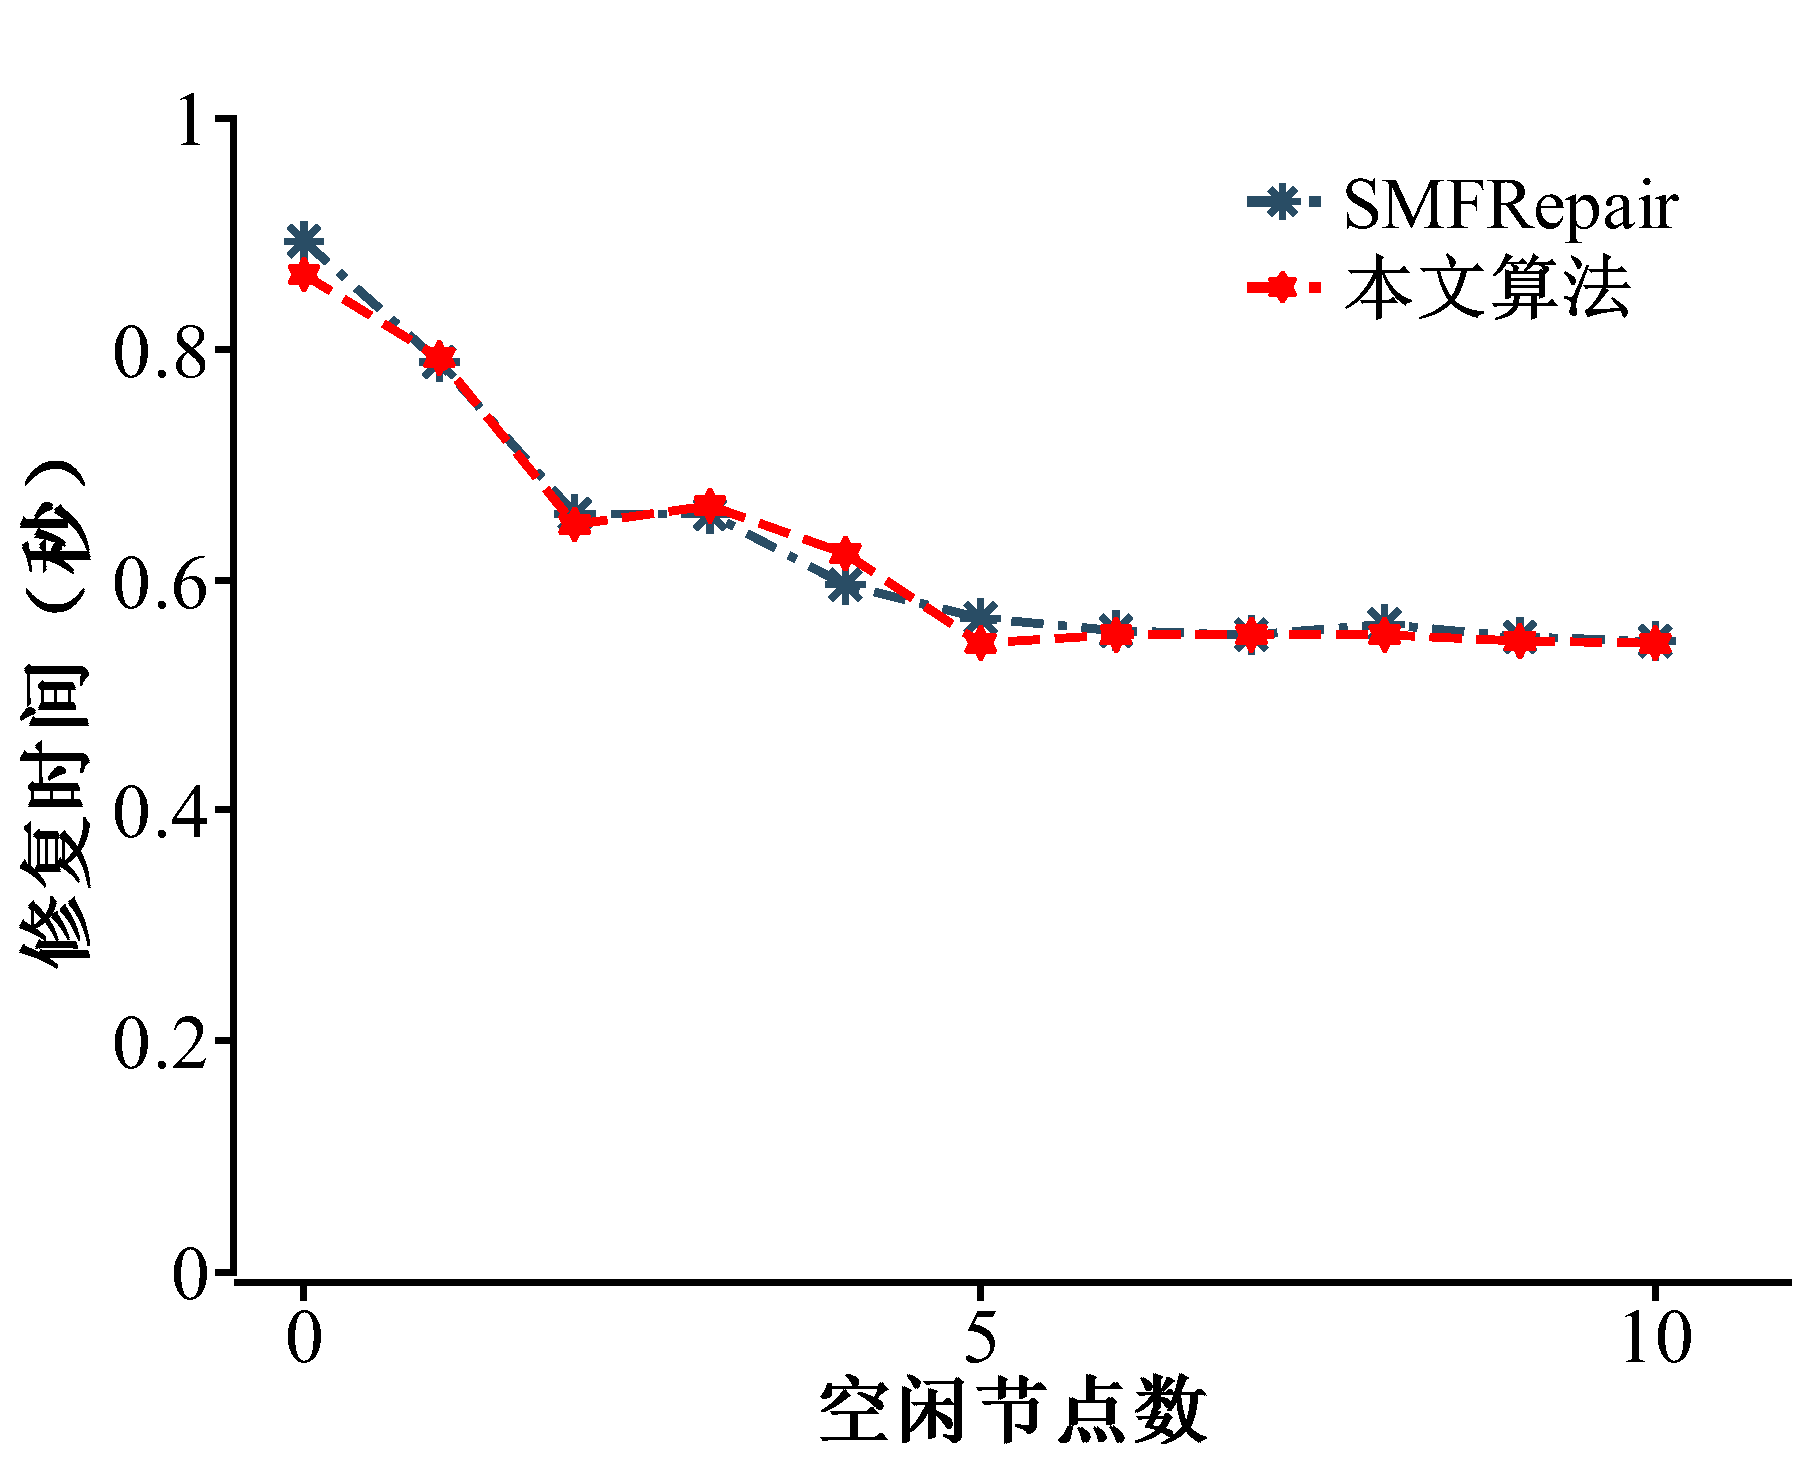
\includegraphics[width=1\linewidth]{figures/3-16.pdf}
		\caption{$RS(n,k)$配置理论结果}
		\label{fig:3-16}
	\end{subfigure}
	\begin{subfigure}[t]{0.4\textwidth}
		\centering
		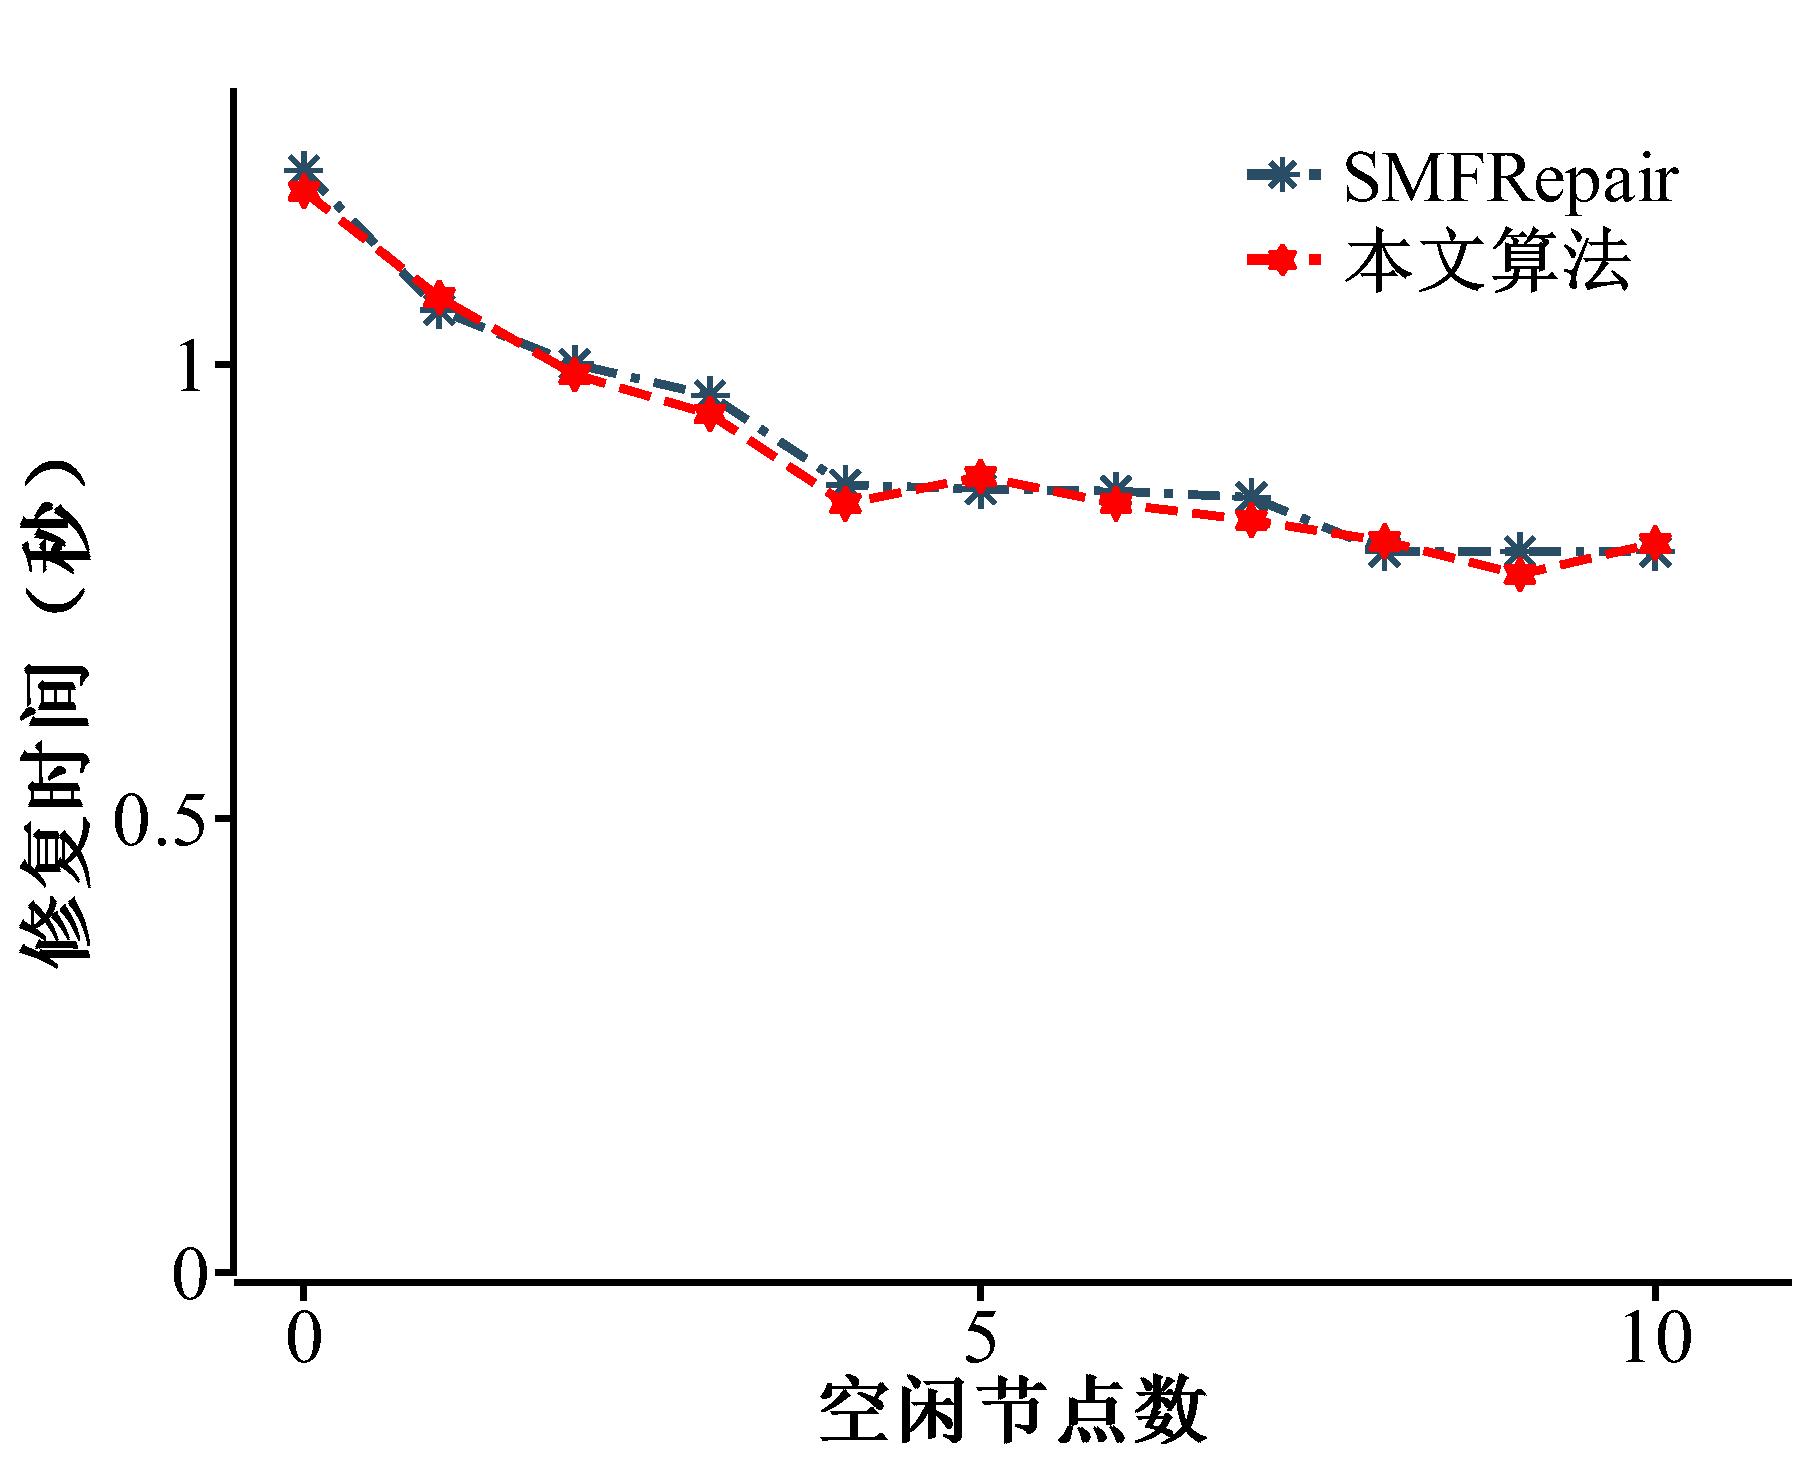
\includegraphics[width=1\linewidth]{figures/3-17.pdf}
		\caption{磁盘带宽$b_d$理论结果}
		\label{fig:3-17}
	\end{subfigure}
	\begin{subfigure}[t]{0.4\textwidth}
		\centering
		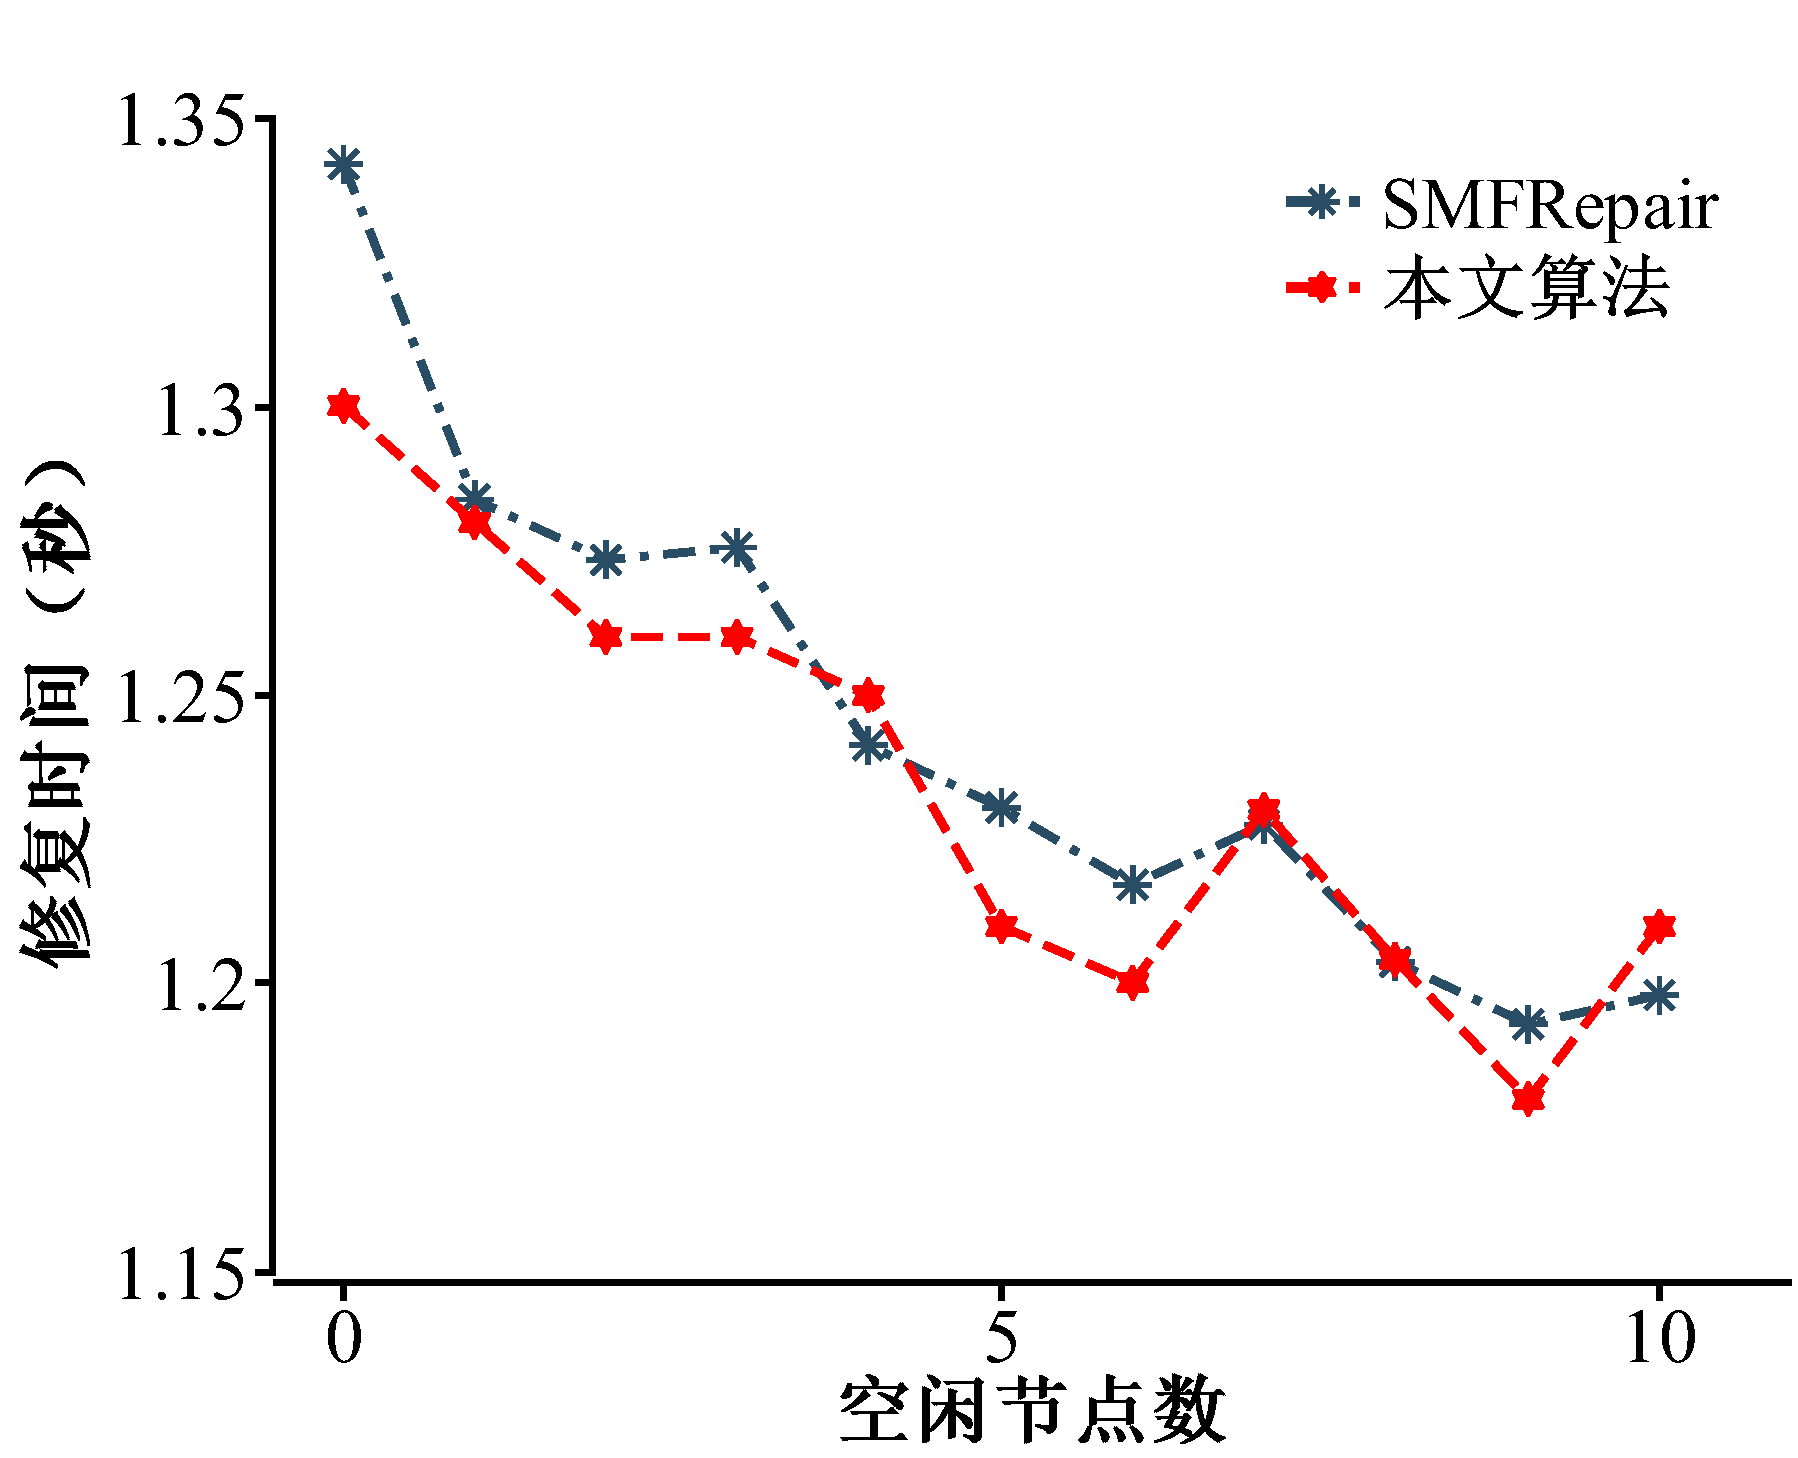
\includegraphics[width=1\linewidth]{figures/3-18.pdf}
		\caption{网络带宽$b_n$理论结果}
		\label{fig:3-18}
	\end{subfigure}
	\caption{预测修复与反应式修复建模对比}
	\label{fig:3-15-18}
\end{figure}




\subsection{带宽变化影响}


\begin{figure}[htbp]
	\centering
	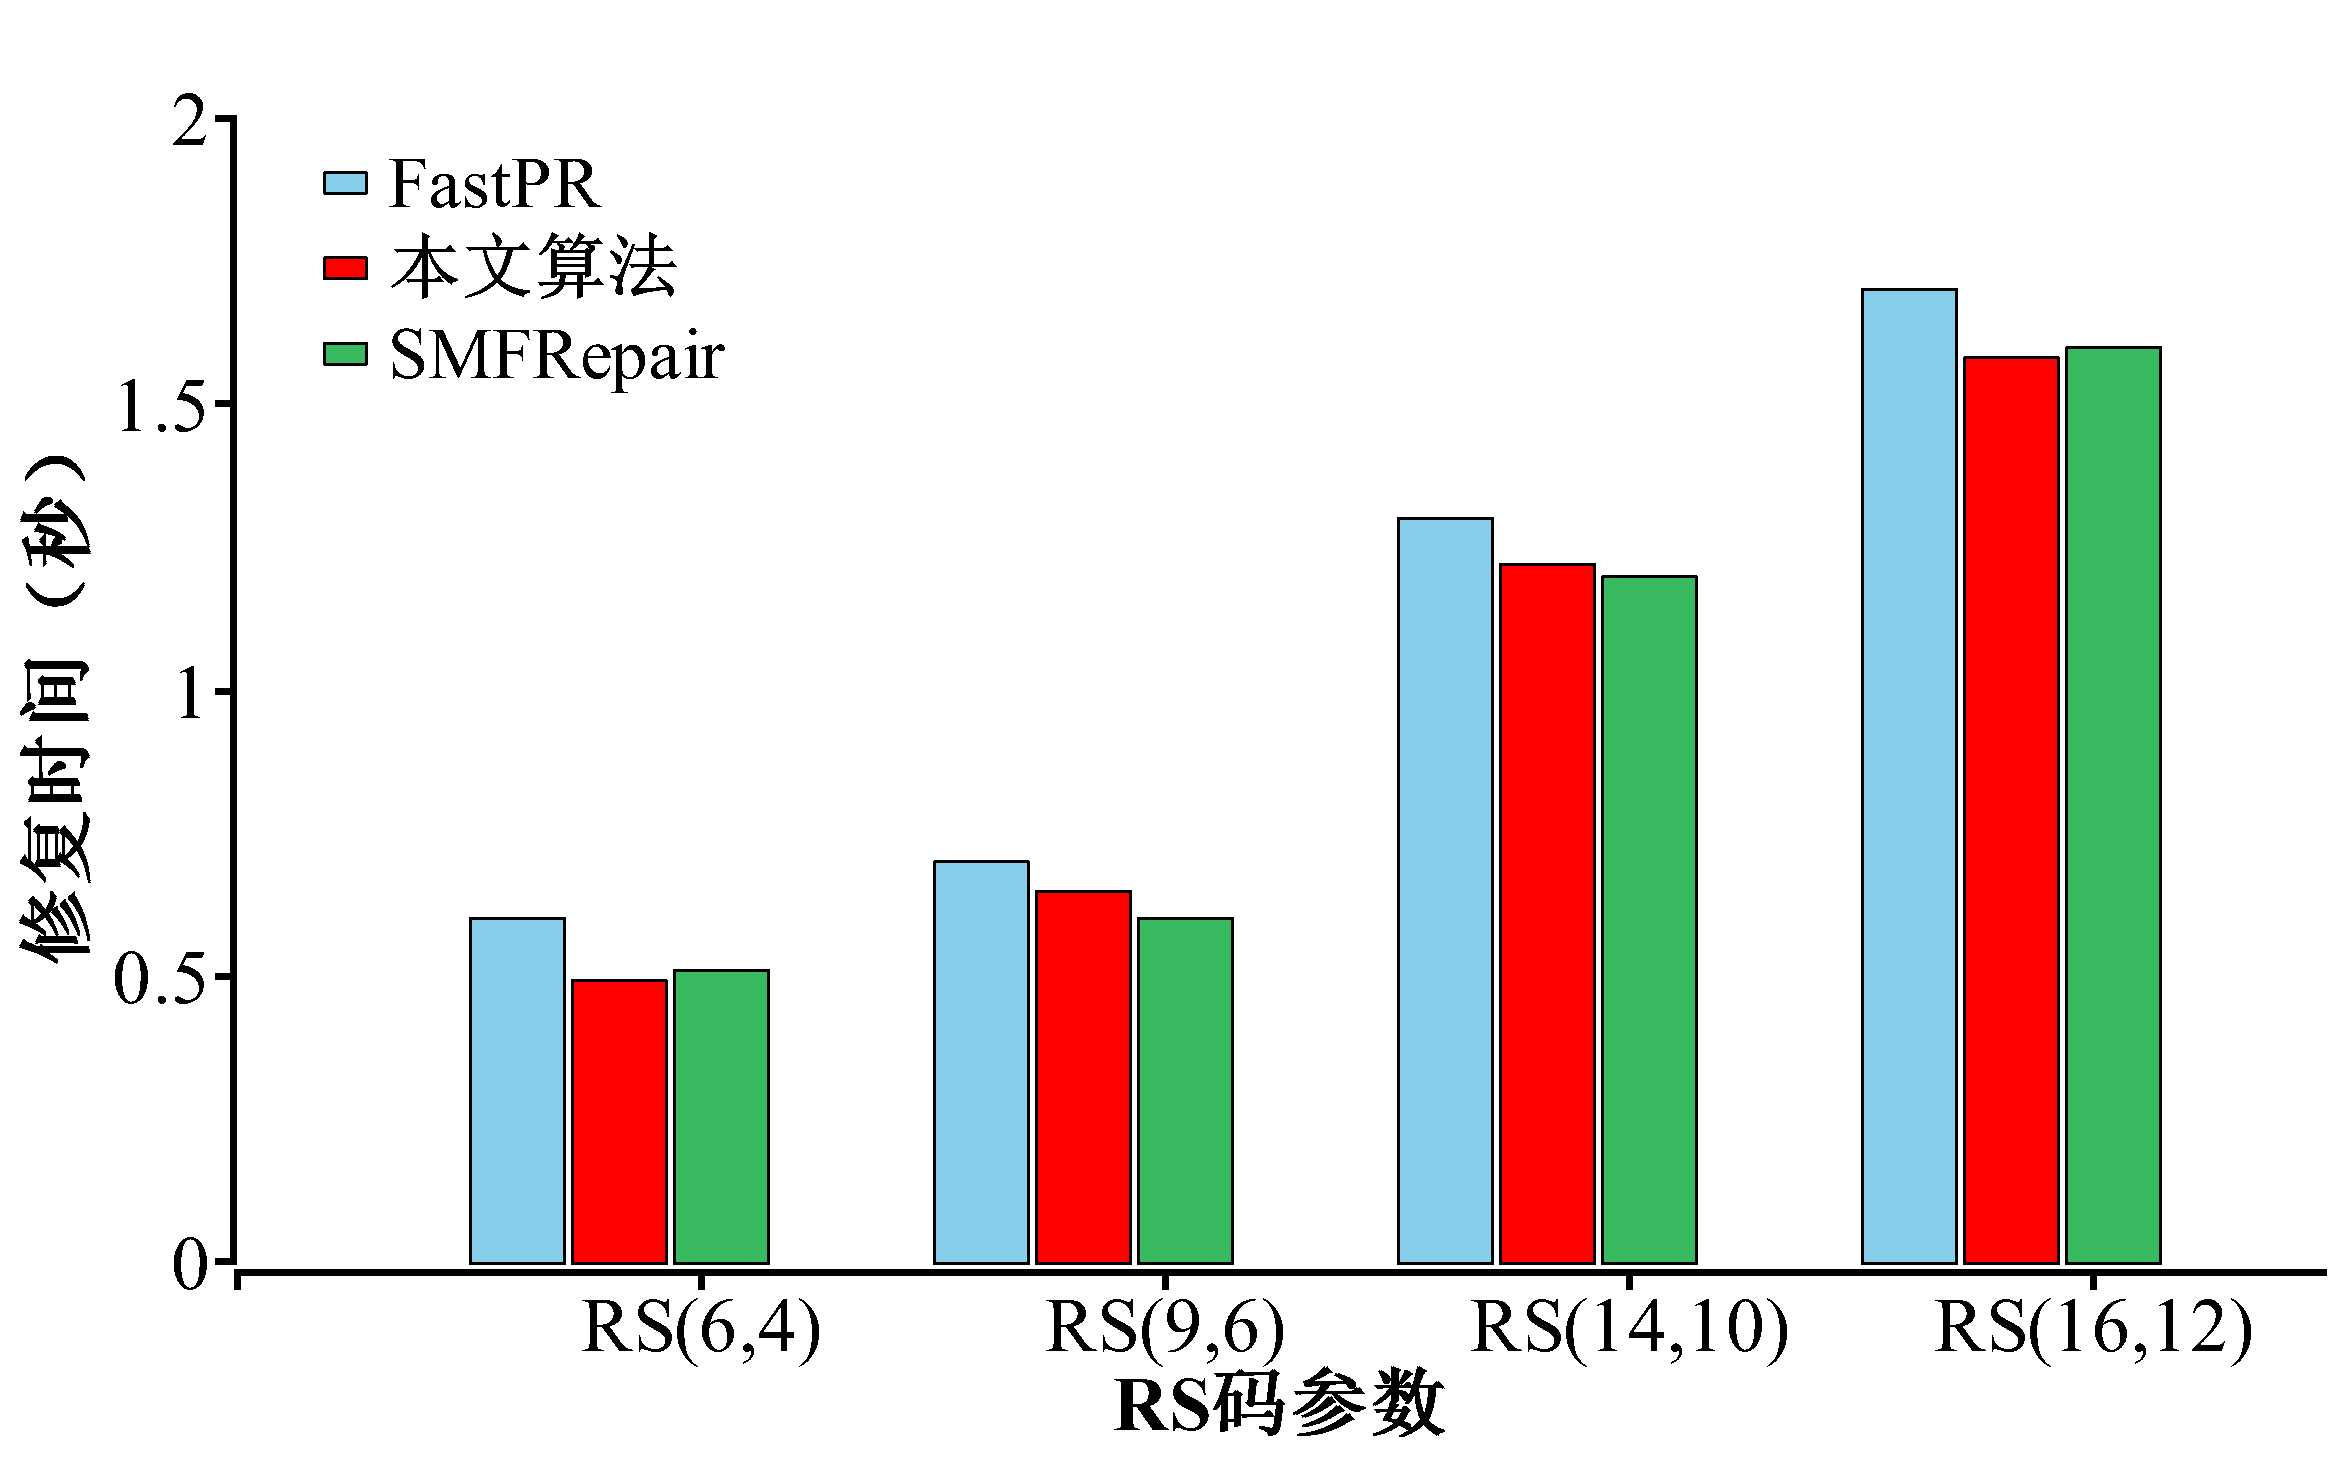
\includegraphics [scale=0.25]{figures/3-19.pdf}
	\caption{节点中继的流程}
	\label{fig:3-19}
\end{figure}
\chapter{基于混合纠删码的数据修复技术研究}

\section{引言}
数据恢复一般有两种技术:重构(reconstruction)和退化读(degraded read)。
重构是指数据已经在存储设备中丢失,在实际的数据修复后
将其存储到新的设备中。 退化读指的是在应对暂时性
故障时,恢复操作读取的数据不必写入到设备中。 研
究一般集中在降低数据修复时所需要读取与传输的数
据量上,缓解高退化读的延迟问题。

在传统的存储系统中大多只采用一种纠删码进行
数据的处理和存储,这种方式一般先将文件分割成固
定大小的数据块,再将这些数据块每$k$
个作为一组,
每组独立进行编码操作生成$n$
个块,其中$n$
个块的集合
称为一个条带(Stripe),然而这种方式难以在保持低
存储空间消耗的情况下降低退化读的延迟时间。最
近,一些系统开始采用多副本技术与纠删码混合或者
混合纠删码的方式来进行数据的存储\cite{ma2013ensemble,friedman2014replicated,xia2015tale}。
\citet{friedman2014replicated,xia2015tale}设计了一种融合了多副本技术和纠删码技术存储系统。
而在\citet{xia2015tale}提出的HACFS中,将从属于同一码种(product code和LRC)但不同参数的纠删码部署到系统中,分别处理冷数据和热数据。
然而,由于选取了同一码族的编码,该码族的既定缺陷将难以避免。
如采用 product code(PC)时,其编码特性使得这一策略无论如何最多允许丢失三个数据块;
而不论是采用PC还是LRC,其存储冷数据时所采用编码均不是MDS的,在存储开销方面存在缺陷。
为了改进此问题,\citet{wang2020adaptive}尝试选取来自不同码族的两种编码,即LRC和HH(Hitchhiker)码来组成混合存储策略。
目的是为了降低系统总体的退化读延迟,且对于热数据采用低恢复延迟的编码,冷数据采取保证MDS特性的编码。然后问题在于,虽然
LRC\&HH码的方案可以通过downcode和upcode的方式将数据存储从两种编码之间进行切换,但却没有良好的自适应负载,亦即
没有针对数据的I/O特点针对性地提出各种负载场景下数据的动态切换方案。

本文在前文预先修复的单一纠删码的基础上,进一步推进了纠删码修复技术的应用。在\citet{wang2020adaptive}工作的基础上,
提出了一种可感知数据热度的负载动态自适应的混合纠删码(LRC\&HH)数据修复方案。
旨在根据真实储存系统数据修复场景中的数据I/O的特点,以及数据访问和故障事件的时空局部性,提出更加符合相应情况的混合纠删码
修复方案,从而对于计算开销型修复任务降低其开销和存储成本,对读取密集型和频繁重建型修复任务降低其工作负载,并加速系统的
修复速度和减少重建时间。

\section{编码策略选择}
为了选择出一对合适的编码策略来适应性地调整数据存储和恢复性能,本文总结了以下要求。
\begin{enumerate}
	\item 两种编码策略应该有类似的布局,更加方便且低成本地建立它们之间的转换;
	\item 两种编码策略应具有较高的灵活性,以支持任意数量的存储节点,并且可以适用于负载平衡的任务要求;
	\item 两种编码策略在数据存储和数据修复任务中分别发挥不同的作用,实现功能上的互补。
\end{enumerate}

\subsection{局部修复码(LRC)}

LRC在传统RS编码的基础上,引入局部分组的思想,将编码块划分成多个小分组,分组内部生成局部校验块进行容错保护。
数据修复不再完全依赖于全局校验组,优先使用局部分组内的数据进行重建,从而通过减少参与节点的数量,降低了修复过程中的网络传输开销和磁盘读取开销。
在LRC中,$m$个冗余块被细分为全局冗余块及局部冗余块,
两者的块数是LRC中的重要参数。记一个LRC编码中全局冗余块的块数为$g$,
局部冗余块的块数为$l$,就有$m = g + l$;这样的一个LRC被记为LRC$(k,l,g)$。在进行
LRC$(k,l,g)$的编码操作时,首先将$k$个数据块通过一个RS$(k,g)$
码编码得到$g$个全局冗余块,
之后将$k$个数据块(相对)平均地分为$l$个组,
每一组将对应一个局部冗余块。 
在每一组中,局部冗余块将通过这一组中的数据块直接进行异或运算得到。

局部冗余块的设置减少了恢复数据时需要访问的节点数。 
当一个数据块需要恢复时,只需要获取它所在分组对应的局部冗余块及分组中其余的数据块,
便可以对它们进行异或运算得出恢复结果。一个LRC$(k,l,g)$恢复一个数据块需要另外$k/l$块,
而对应的一个RS$(k,g)$码则需要$k$块,是前者的$l$倍。如图~\ref{fig:4.1}所示,是LRC$(6,2,2)$的具体组合方式,
其中$p_x$和$p_y$是两个全局冗余块,而两个数据块被平均地分为了三组$(x_1,x_2)$,$(y_1,y_2)$,$(z_1,z_2)$,它们
分别对应的局部冗余块为$p_{xy}$和$p_{yz}$。当$x_1$需要被修复时,只需要获取$x_2,y_1$和$p_{xy}$即可。


\begin{figure}[htbp]
	\centering
	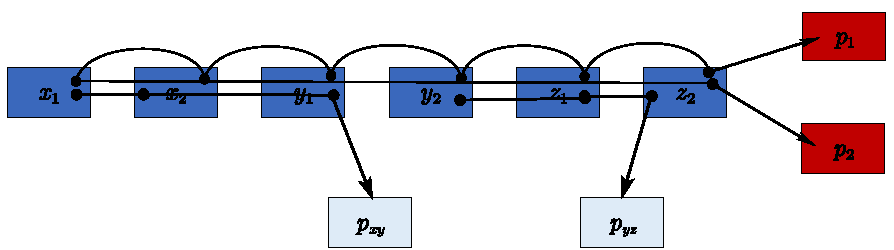
\includegraphics [scale=0.7]{figures/4.1.pdf}
	\caption{LRC(6,2,2)的组成}
	\label{fig:4.1}
\end{figure}

\subsection{Hitchhiker(HH)码}

在一个HH$(k,m)$码中,每个条带被分为两个子条带,分别为$a={a_i}$和$b={b_i}$,
且其中有$k$个数据块和$m$个校验块。在编码计算中,同一个子条带中的数据首先会被编码成RS$(k,m)$,从而得到校验块
$f_i(a)$和$f_i(b)(1\leqslant i\leqslant m)$。然后,将子条带$a$中的$k$个数据块平均地分为$(m-1)$组,每个组
$G_i$对应子条带$b$中的校验块$b_{k+i+1}$,最后将$G_i$和$f_{i+1}(a)$中的数据块进行XOR计算。

在丢失一个数据块时,
设其在$a$中的子数据块在上述分组中对应$g_t(a)$。
首先通过子条带$b$中可用的另外$(k-1)$个数据块以及$f_1(b)$,可以恢复得到丢
失的在$b$中的子数据块,进而可以求出$f_{(t-k)}(b)$。而$a$中子数据块
则可以通过上述分组中同一组内其余的$a$中子数据块,子条带$b$的第$t$个子块,
以及刚刚求出的$f_{(t-k)}(b)$进行异或运算得到。 
这样,要恢复一个数据块,需要读取的子数据块数为$k+\frac{k}{m-1}=\frac{km}{m-1}$,
折合为$\frac{km}{2(m-1)}$块,相比于RS码需要$k$块,在$m \geqslant 3$时均有较为明显的减少。

如图~\ref{fig:4.2}所示,展示的是HH$(12,4)$组成,如果想修复$a_1$和$b_1$,首先需要读取$b_2$到$b_{13}$总共12个数据块。
这12个数据块足以恢复出$b_1$,然后可以计算出$b_{14}$对应的RS校验块$f_2(b)$。
最后,再读取$a_2$到$a_4$和$b_{14}$,计算出$a_1=a_2\oplus a_3 \oplus a_4 \oplus b_{14} \oplus f_2(b)$。
总共需要读取16个数据块,相比RS码少读了8个数据块。

\begin{figure}[htbp]
	\centering
	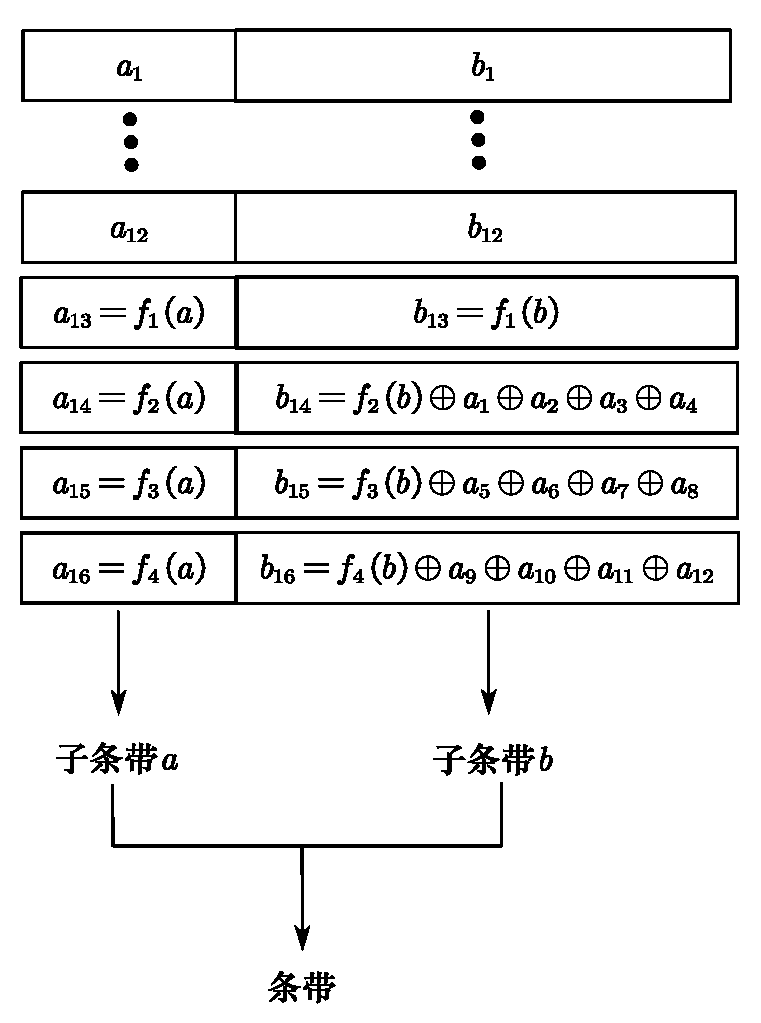
\includegraphics [scale=0.5]{figures/4.2.pdf}
	\caption{HH$(12,4)$码组成}
	\label{fig:4.2}
\end{figure}

\section{负载自适应策略}
\label{Section:4.3}

受\citet{qiu2020ec}工作的启发,针对实际存储系统数据I/O的特点,本文静态地将数据分为六类(如表~\ref{table:4-1}所示),其中风险指的是因数据丢失而产生对系统风险的影响。
1)低风险的冷数据;2)高风险的冷数据;3)低风险的写入密集型数据;
4)高风险的写入密集型数据;5)低风险的读取密集型数据;6)高风险的读取密集型数据。
其中,读取密集型和写入密集型数据都属于热数据,而读写平衡的系统应用可以属于写入密集型或读取密集型。
一般来说在低风险环境下,这种应用更可能是写入密集型的,因为整体性能主要受写入操作的影响。
然后可以确定为其分配何种编码,并为数据的动态I/O提供自适应方法。

\begin{table}[htbp]
	% \setlength{\tabcolsep}{2.9pt}
	\centering
	\caption{不同系统负载情况下的编码分配方案}
	\begin{tabular}{cccc}
		\toprule
        \multicolumn{2}{c}{\multirow{2}*{编码策略}}          & \multicolumn{2}{c}{修复负载} \\
         &                                      & 高风险             & 低风险    \\[2pt]
        \hline
		\\[-15pt]
        \multirow{3}{*}{系统负载} & 写入密集型 & LRC或HH & Hitchhiker  \\
                                                & 读取密集型 & LRC & Hitchhiker  \\
                                                & 冷数据 & Hitchhiker & Hitchhiker  \\
		\midrule
	\end{tabular}
	\label{table:4-1}
\end{table}



\subsection{编码分配规则}
\label{subsection:4.1}
为了让不同的数据和读写任务工作负载情况匹配上适当的编码方案,
显然可以得到如表~\ref{table:4-1}中总结了编码分配策略。直观地说,冷数据或低风险数据可以选择存储开销较低的HH码,
这样可以保持较高的存储效率,以及良好的系统可靠性。特别是对于写入密集型I/O的任务,
而对于具有高故障风险且以读为主的数据,LRC码可以节省大量的重建带宽,并对I/O速度造成更少的负面影响。
然而,对于高风险的写入密集型数据,难以选择一个合适的编码策略,因需要在系统的读取性能和修复I/O之间进行平衡,
从而确定合适的编码来最大化系统的整体性能。为了解决这个问题,本文进行了如下计算,最终结果呈现在表~\ref{table:4-2}。

\textbf{读写负载模式}。首先确定RS$(k,r)$在单个数据块上的计算性能消耗$RWCost_{compute}^{RS}$,
磁盘I/O消耗$RWCost_{I/O}^{RS}$,传输消耗$RWCost_{transmission}^{RS}$。
设系统读写调度的写入速度为$v_w$,读取速度为$v_r$,一个数据块大小为$\gamma$,那么对于
RS$(k,r)$而言,其编码过程中的GF运算次数等价于运算复杂度即$k \times r$,而对于读写交叉的任务而言其所占据的比例为$\frac{v_w}{v_w+v_r}$,
故在读写负载模式中RS$(k,r)$的计算性能消耗$RWCost_{compute}^{RS}$为:
\begin{equation}
	\label{eq:4-1}
	RWCost_{compute}^{RS} = \frac{v_w}{v_w+v_r} \gamma kr
\end{equation}
这里令$\frac{v_w}{v_r}$为$\beta$,则式~\ref{eq:4-1}可改写为:

\begin{equation}
	\label{eq:4-2}
	RWCost_{compute}^{RS} = \frac{\beta}{1+\beta} \gamma kr
\end{equation}

设磁盘一次I/O可传输的字节数为$\phi$,则可得到读写负载模式中RS$(k,r)$的磁盘I/O消耗$RWCost_{I/O}^{RS}$为:
\begin{equation}
	\label{eq:4-3}
	RWCost_{I/O}^{RS} = \frac{\gamma}{\phi}
\end{equation}

对于传输消耗$RWCost_{transmission}^{RS}$,分为读取传输和写入传输,其中读取任务的传输消耗为$\frac{v_r}{v_r+v_w}$,
写入任务的传输消耗为$\frac{v_w\frac{r+k}{k}}{v_r+v_w}$。那么读写负载模式中RS$(k,r)$的
传输消耗$RWCost_{transmission}^{RS}$为:

\begin{equation}
	\begin{aligned}
	\label{eq:4-4}
	RWCost_{transmission}^{RS} & = \frac{v_r}{v_r+v_w} + \frac{v_w\frac{r+k}{k}}{v_r+v_w} \\
	                    & = \frac{1}{1+\beta} + \frac{\beta}{1+\beta} \cdot \frac{r+k}{k} \\
						& = \frac{\beta(r+k)+k}{k(1 + \beta)} \\
						& = 1 + \frac{\beta}{1 + \beta} \cdot \frac{r}{k}
	\end{aligned}
\end{equation}

由于LRC$(k,l,g)$恢复一个数据块需要另外$k/l$块,
而对应的一个RS$(k,g)$码则需要$k$块,是前者的$l$倍。
故将其分别代入式~\ref{eq:4-2},式~\ref{eq:4-3},式~\ref{eq:4-4},则可以得到读写负载模式中LRC$(k,l,g)$的
计算性能消耗$RWCost_{compute}^{LRC}$,
磁盘I/O消耗$RWCost_{I/O}^{LRC}$,传输消耗$RWCost_{transmission}^{LRC}$分别为:
\begin{equation}
	\label{eq:4-5}
	RWCost_{compute}^{LRC} = \frac{\beta}{l(1+\beta)} \gamma kr
\end{equation}
\begin{equation}
	\label{eq:4-6}
	RWCost_{I/O}^{LRC} = \frac{\gamma}{\phi}
\end{equation}
\begin{equation}
	\label{eq:4-7}
	RWCost_{transmission}^{LRC} = 1 + \frac{\beta}{k(1 + \beta)} \cdot rl
\end{equation}

同样,对于HH码,其需要读取$\frac{km}{2(m-1)}$块数据进行处理,分别将其代入式~\ref{eq:4-2},式~\ref{eq:4-3},式~\ref{eq:4-4},
则可以得到读写负载模式中HH$(k,m)$的
计算性能消耗$RWCost_{compute}^{HH}$,
磁盘I/O消耗$RWCost_{I/O}^{HH}$,传输消耗$RWCost_{transmission}^{HH}$分别为:
\begin{equation}
	\label{eq:4-8}
	RWCost_{compute}^{HH} = \frac{\gamma \beta kmr}{2(1+\beta)(m-1)}
\end{equation}
\begin{equation}
	\label{eq:4-9}
	RWCost_{I/O}^{HH} = \frac{\gamma}{\phi}
\end{equation}
\begin{equation}
	\label{eq:4-10}
	RWCost_{transmission}^{HH} = 1 + \frac{\beta}{1 + \beta} \cdot \frac{2r(m-1)}{km}
\end{equation}


\textbf{修复负载模式}。与读写模式相同,首先确定RS$(k,r)$在修复负载模式下单个数据块上的计算性能消耗$RecoverCost_{compute}^{RS}$,
磁盘I/O消耗$RecoverCost_{I/O}^{RS}$,传输消耗$RecoverCost_{transmission}^{RS}$。
因在修复过程中需要传输$k$个数据块和$(r+k)\times r \times r$\cite{qiu2020ec}次运算,故修复负载模式下的RS$(n,k)$的计算性能消耗$RecoverCost_{compute}^{RS}$为:
\begin{equation}
	\label{eq:4-11}
	RecoverCost_{compute}^{RS} = (r+k)r^2+\gamma k
\end{equation}
同样可得,修复负载模式下的RS$(n,k)$的磁盘I/O消耗$RecoverCost_{I/O}^{RS}$为:

\begin{equation}
	\label{eq:4-12}
	RecoverCost_{I/O}^{RS} = \frac{\gamma}{\phi}
\end{equation}
显然,修复时需要传输$k$个数据块,则传输消耗$RecoverCost_{transmission}^{RS}$为:
\begin{equation}
	\label{eq:4-13}
	RecoverCost_{transmission}^{RS} = k
\end{equation}

同理,分别将LRC码的$\frac{k}{l}$和HH码的$\frac{km}{2(m-1)}$代入到式~\ref{eq:4-11},~\ref{eq:4-12},~\ref{eq:4-13},可得
修复负载模式中LRC$(k,l,g)$的
计算性能消耗$RecoverCost_{compute}^{LRC}$,
磁盘I/O消耗$RecoverCost_{I/O}^{LRC}$,传输消耗$RecoverCost_{transmission}^{LRC}$分别为:
\begin{equation}
	\label{eq:4-14}
	RecoverCost_{compute}^{LRC} = r^3 + \frac{kr^2}{l} + \frac{k\gamma}{l}
\end{equation}
\begin{equation}
	\label{eq:4-15}
	RecoverCost_{I/O}^{LRC} = \frac{\gamma}{\phi}
\end{equation}
\begin{equation}
	\label{eq:4-16}
	RecoverCost_{transmission}^{LRC} = \frac{k}{l}
\end{equation}

修复负载模式中HH$(k,m)$的
计算性能消耗和磁盘I/O消耗$RecoverCost_{compute}^{HH}$、
$RecoverCost_{I/O}^{HH}$,传输消耗$RecoverCost_{transmission}^{HH}$分别为:
\begin{equation}
	\label{eq:4-17}
	RecoverCost_{compute}^{HH} = r^3 + \frac{km(r^2+\gamma)}{2(m-1)}
\end{equation}
\begin{equation}
	\label{eq:4-18}
	RecoverCost_{I/O}^{HH} = \frac{\gamma}{\phi}
\end{equation}
\begin{equation}
	\label{eq:4-19}
	RecoverCost_{transmission}^{HH} = \frac{km}{2(m-1)}
\end{equation}

最终,读写负载模式和修复负载模式下的LRC和HH各种任务的消耗计算如表~\ref{table:4-2}所示。
\begin{table}[htbp]
	% \setlength{\tabcolsep}{2.9pt}
	\centering
	\caption{不同系统负载情况下的编码分配方案}
	\begin{tabular}{clcc}
		\toprule
        \multicolumn{2}{c}{\multirow{1}*{编码策略}}  & LRC$(k,l,g)$             & HH$(k,m)$    \\[2pt]
        \hline
		\\[-15pt]
        \multirow{3}{*}{读写负载模式} & $RWCost_{compute}$ & $\frac{\beta}{l(1+\beta)} \gamma kr$ & $\frac{\gamma \beta kmr}{2(1+\beta)(m-1)}$  \\
                                & $RWCost_{I/O}$ & $\frac{\gamma}{\phi}$ & $\frac{\gamma}{\phi}$  \\
                                & $RWCost_{transmission}$ & $1 + \frac{\beta}{k(1 + \beta)} \cdot rl$ & $1 + \frac{\beta}{1 + \beta} \cdot \frac{2r(m-1)}{km}$  \\
        \hline
        \\[-15pt]                        
        \multirow{3}{*}{修复负载模式} & $RecoverCost_{compute}$ & $r^3 + \frac{kr^2}{l} + \frac{k\gamma}{l}$ & $r^3 + \frac{km(r^2+\gamma)}{2(m-1)}$  \\
        & $RecoverCost_{I/O}$ & $\frac{\gamma}{\phi}$ & $\frac{\gamma}{\phi}$  \\
        & $RecoverCost_{transmission}$ & $\frac{k}{l}$ & $\frac{km}{2(m-1)}$  \\
		\midrule
	\end{tabular}
	\label{table:4-2}
\end{table}



设$\alpha$为系统进行XOR计算的速度(次/s),$\lambda$为网络中传输的数据量(bytes/s)
,故可得相应编码的写读开销$W$和$R$分别为:

\begin{equation}
	\begin{aligned}
	\label{eq:4-22}
	W & = RWCost_{compute} \cdot \frac{1+\beta}{\beta} \cdot \frac{1}{\alpha} \\
	  & + RWCost_{I/O} \\
	  & + \frac{\gamma}{\lambda} (RWCost_{transmission} - \frac{1}{1+\beta}) \cdot \frac{1+\beta}{\beta}
	\end{aligned}
\end{equation}

\begin{equation}
	\begin{aligned}
	\label{eq:4-23}
	R & = \frac{RecoverCost_{compute}}{\alpha} \\
	& +  RecoverCost_{I/O}  \\
	& +  \frac{\gamma RecoverCost_{transmission}}{\lambda}
	\end{aligned}
\end{equation}
基于表~\ref{table:4-2}和式~\ref{eq:4-22},式~\ref{eq:4-23}可以为LRC码和HH码定义如下变量:

% \begin{equation}
% 	\label{eq:4-20}
% 	W_{LRC} = \gamma (\frac{kr}{\alpha l} + \frac{k+rl}{k \lambda} + \frac{\gamma}{\phi})
% \end{equation}

% \begin{equation}
% 	\label{eq:4-21}
% 	R_{LRC} = \frac{r^3 + \frac{kr^2}{l} + \frac{k\gamma}{l}}{\alpha} + \gamma (\frac{k}{\lambda l} + \frac{1}{\phi})
% \end{equation}

% \begin{equation}
% 	\label{eq:4-24}
% 	W_{HH} = \frac{\gamma kmr}{2\alpha (m-1)} + \frac{\gamma}{\lambda} (1 + \frac{2r(m-1)}{km}) + \frac{\gamma}{\phi}
% \end{equation}

% \begin{equation}
% 	\label{eq:4-25}
% 	R_{HH} = \frac{r^3}{\alpha} + \frac{km(r^2+\gamma)}{2 \alpha (m-1)} + \frac{\gamma}{\phi} + \frac{km \gamma }{2 \lambda (m-1)}
% \end{equation}


\begin{equation}
	\begin{aligned}
	\label{eq:4-20}
	W_{LRC} & = \gamma (\frac{kr}{\alpha l} + \frac{k+rl}{k \lambda} + \frac{\gamma}{\phi}) \\
	R_{LRC} & = \frac{r^3 + \frac{kr^2}{l} + \frac{k\gamma}{l}}{\alpha} + \gamma (\frac{k}{\lambda l} + \frac{1}{\phi}) \\
	W_{HH} & = \frac{\gamma kmr}{2\alpha (m-1)} + \frac{\gamma}{\lambda} (1 + \frac{2r(m-1)}{km}) + \frac{\gamma}{\phi} \\
	R_{HH} & = \frac{r^3}{\alpha} + \frac{km(r^2+\gamma)}{2 \alpha (m-1)} + \frac{\gamma}{\phi} + \frac{km \gamma }{2 \lambda (m-1)}
	\end{aligned}
\end{equation}
% 由式~\ref{eq:4-20},式~\ref{eq:4-21},式~\ref{eq:4-24},式~\ref{eq:4-25},可以得到如下不等式来决定
由式~\ref{eq:4-20},可以得到如下不等式来决定
编码的选择:


\begin{equation}
	\label{eq:4-26}
	\delta=\frac{\text { writes }}{\text { recoveries }} \geq \frac{R_{LRC}-R_{HH}}{W_{HH}-W_{LRC}}=\eta
\end{equation}
当$\delta \geqslant \eta$时,意味着瓶颈性能主要受到写需求的影响,所以选用HH码更加合适;
否则重建带宽就是最大的影响因素,那么LRC码则是更好的选择。在实践中\cite{qiu2020ec},为了
缓解频繁切换编码策略所产生的开销,将不等式~\ref{eq:4-26}调整为下式:
\begin{equation}
	\label{eq:4-27}
	\delta \geqslant \eta+\Delta \text {\,或\,} \delta \leqslant \eta-\Delta(0 \leqslant \Delta<\eta)
\end{equation}




\subsection{自适应选择算法}

随着系统的运行,数据的冷热属性会不断地进行切换。为此需要构造相应的冷热数据划分算法,
记录数据访问发生失败时的时间和节点位置,利用这些信息可以使用LRU算法来为冷热数据划分定制自适应选择算法。
定义两个队列分别用于正常读取模式和故障模式,将缓存算法应用于队列,具体如图~\ref{fig:4.3}所示,
根据HACFS\cite{xia2015tale}用Fast Code和Compact Code指代对应的两种编码方式,相应地分别对应
LRC码和HH码。

\begin{figure}[htbp]
	\centering
	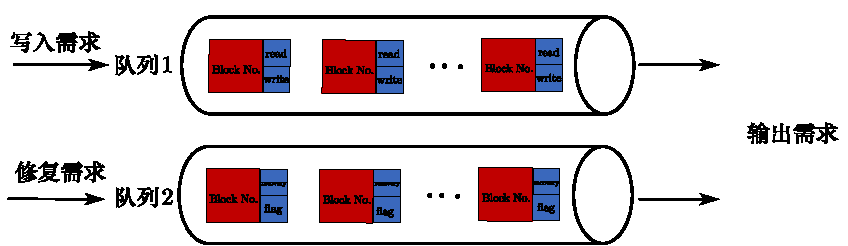
\includegraphics [scale=0.7]{figures/4.3.pdf}
	\caption{动态自适应划分冷热数据队列}
	\label{fig:4.3}
\end{figure}

用队列1来记录数据写入的信息流,其中每个块记录了块ID和缓存命中次数。
队列2存储着数据块的恢复请求,其中包含了区块ID、缓存命中次数和表示数据的编码方案。
首先将LRC$(k, l,g)$设定为整个存储系统的默认编码,两个队列在启动后会有一个默认初始化,
在自适应规则中,三个条件来触发自适应过程。 首先,对于在队列2头部插入的每个修复请求,
算法确定相关块是否需要用LRC码进行编码。 其次,对于在队列1头部插入的每个写请求,
算法确定相关的块是否需要用HH码进行编码。 最后,对于在队列2尾部删除的每个修复请求,
算法会将LRC码转换成HH码。具体的过程如算法~\ref{alg:4-1}中所示。

\begin{algorithm}[htpb]
	\begin{algorithmic}[1]
		% \newlength{\commentindent}
		\setlength{\commentindent}{.3\textwidth}
		\setlength{\algorithmicindent}{1.5em}
		\renewcommand{\algorithmiccomment}[1]{\unskip\hfill\makebox[\commentindent][l]{$\rhd$~#1}\par}
		\LetLtxMacro{\oldalgorithmic}{\algorithmic}
		\renewcommand{\algorithmic}[1][0]{
			\oldalgorithmic[#1]
			\renewcommand{\ALC@com}[1]{
				\IFnum\pdfstrcmp{##1}{default}=0\ELSE\algorithmiccomment{##1}\fi}%
		}
		\REQUIRE{Queue1,Queue2 and $\eta$}
		% \ENSURE{$\textbf{NewW}$}
        \FOR{\text{Queue2头的每个插入请求}}
        \IF{flag $\neq $ LRC and (writes/recoveries) $< \eta$}
        \STATE set flag = LRC;
        \STATE convert to LRC;
        \ENDIF
        \ENDFOR
        \FOR{\text{Queue1头的每个插入请求}}
        \IF{flag $\neq $ HH and (writes/recoveries) $\geqslant  \eta$}
        \STATE set flag = HH;
        \STATE convert to HH;
        \ENDIF
        \ENDFOR
        \FOR{\text{Queue2尾的每个弹出请求}}
        \IF{flag == LRC }
        \STATE set flag = HH;
        \STATE convert back to HH;
        \ENDIF
        \ENDFOR
		% \STATE $\textbf{NewW} = \textbf{w}$;
		% \WHILE {true}
		% \STATE R = FindMaxTimeRoad($\textbf{NewW}$);
		% \IF {type == 1}
		% \STATE S = FindNodeWithoutChunk($\textbf{NewW}$);
		% \STATE D = R.Destination;
		% \ELSE
		% \STATE S, D = R.Source, R.Destination;
		% \ENDIF
		% \STATE RIdle = GetIdleNode(R);
		% \STATE NewR = DijkstraMinTimeRoad(S, D, RIdle);
		% \STATE Update($\textbf{NewW}$, NewR);
		% \IF {FindMaxTimeRoad($\textbf{NewW}$) == R}
		% \STATE break;
		% \ENDIF
		% \ENDWHILE
		% \STATE $\textbf{return}$ $\textbf{NewW}$;
	\end{algorithmic}
	\caption{动态自适应冷热数据划分算法}
	\label{alg:4-1}
\end{algorithm}


\section{编码切换算法}

HH码和LRC码均为RS码的一种改进。在使用HH$(k,m)$码进行编码时,首先需要进行RS$(k,m)$码
的编码,在进行一系列Piggybacking框架中关于$g_i(a)$的异或运算;而在使用LRC$(k,l,g)$进行编码
时,$g$个全局冗余块需要通过执行RS$(k,g)$码的编码函数得到,而$l$个局部冗余块则需要进行异或运算得到。
另外HH$(k,m)$码中的$g_i(a)$的计算,需要将$k$个数据块分为$(m-1)$组,而LRC$(k,l,g)$中的局部冗余的
计算,则需要将$k$个数据块分为$l$组。由此,当$k_{HH}=k_{LRC}$且$m_{HH}=g_{LRC}$且$m_{HH}-1=l_{LRC}$时,
相应的HH码和LRC码可以共用一个RS码的冗余块,并且可以进行高效地切换。

记$k=k_{HH}=k_{LRC}$以及$t=m_{HH}=g_{LRC}$,则$l_{LRC}=m_{HH}-1=t-1$,系统中采用HH$(k,t)$和LRC$(k,t-1,t)$。
由于HH码会将原RS码中每两个条带视为一个条带中的两个子条带,因此此切换算法也对LRC进行类似处理,即每一个条带中都包含两个
子条带。在LRC中,一个条带中的两个子条带分别进行各自的编码;而在HH码中,其中一个条带$a$的额外冗余信息$g_i(a)$会被
异或到另一子条带$b$的冗余子块中。

从LRC$(k,t-1,t)$转换为HH$(k,t)$码时,
首先将子条带$a$中的各局部冗余子块读取并传输到对应的全局冗余块所在节点,并与该节点中子条带b的全局冗余子块进行异或运算,
之后再将各局部冗余块删除即可。详细过程如算法~\ref{alg:4-2}和图~\ref{fig:4.4}所示。

\begin{figure}[H]
	\centering
	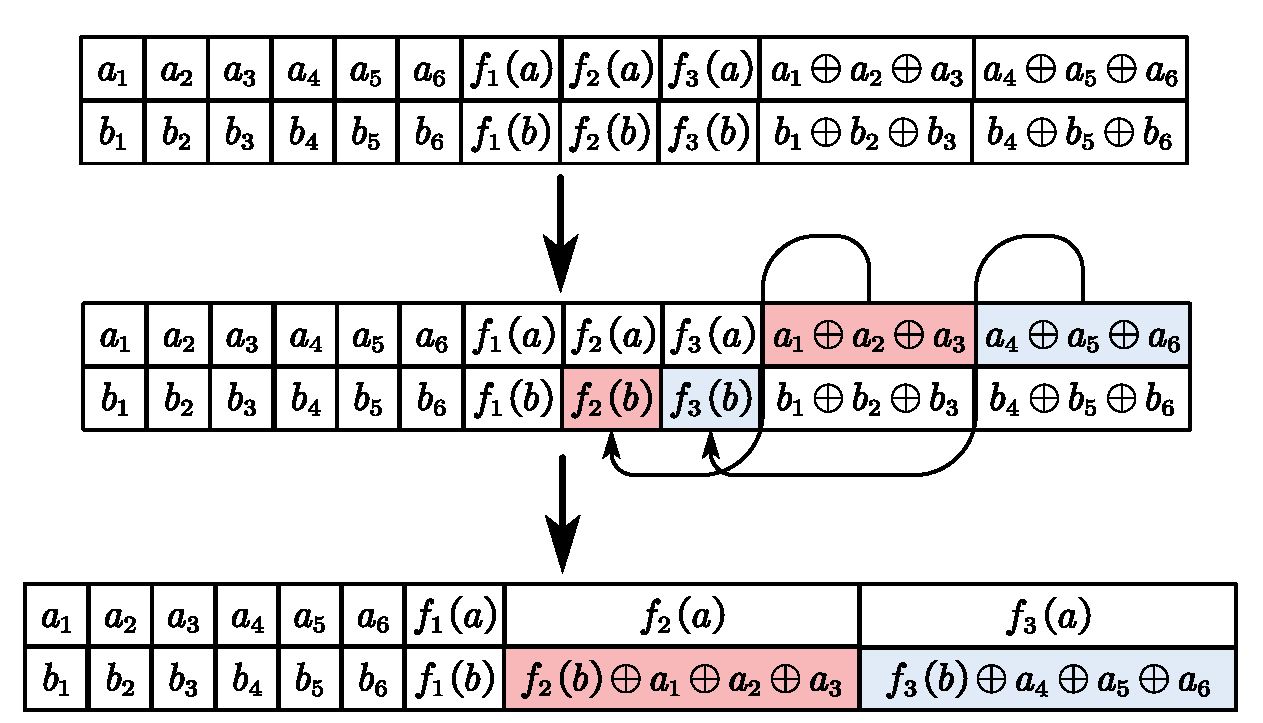
\includegraphics [scale=0.5]{figures/4.4.pdf}
	\caption{LRC$(6,2,3)\rightarrow $ HH$(6,3)$过程}
	\label{fig:4.4}
\end{figure}


\begin{algorithm}[htbp]
	\begin{algorithmic}[1]
		% \newlength{\commentindent}
		\setlength{\commentindent}{.3\textwidth}
		\setlength{\algorithmicindent}{1.5em}
		\renewcommand{\algorithmiccomment}[1]{\unskip\hfill\makebox[\commentindent][l]{$\rhd$~#1}\par}
		\LetLtxMacro{\oldalgorithmic}{\algorithmic}
		\renewcommand{\algorithmic}[1][0]{
			\oldalgorithmic[#1]
			\renewcommand{\ALC@com}[1]{
				\IFnum\pdfstrcmp{##1}{default}=0\ELSE\algorithmiccomment{##1}\fi}%
		}
		\REQUIRE{LRC中的两个子条带$a$和$b$}
		\ENSURE{HH码中的两个子条带$s_a$和$s_b$}
        \STATE $s_a.data := a.data$
        \STATE $s_b.data := b.data$
        \STATE $s_a.parity := a.global$\_$parity$
        \STATE $s_b.parity[1] := b.global$\_$parity[1]$
        \FOR{$i:=2 \, to \, t$}
        \STATE $s_b.parity[i] := b.global$\_$parity[i] \oplus a.local$\_$parity[i-1]$
        \ENDFOR
	\end{algorithmic}
	\caption{LRC$(k,t-1,t)\rightarrow $ HH$(k,t)$算法}
	\label{alg:4-2}
\end{algorithm}


从HH$(k,t)$码转换为LRC$(k,t-1,t)$时,首先计算出所有局部冗余块,
之后再将其中子条带$a$中的局部冗余子块传到对应的全局冗余块所在节点, 
并与该节点中子条带$b$的全局冗余子块进行异或运算,使得这些子条带$b$的全局冗余子块不再包含子条带$a$中
的额外冗余信息$g_i(a)$。详细过程如算法~\ref{alg:4-3}和图~\ref{fig:4.5}所示。


\begin{algorithm}[tb!]
	\begin{algorithmic}[1]
		% \newlength{\commentindent}
		\setlength{\commentindent}{.3\textwidth}
		\setlength{\algorithmicindent}{1.5em}
		\renewcommand{\algorithmiccomment}[1]{\unskip\hfill\makebox[\commentindent][l]{$\rhd$~#1}\par}
		\LetLtxMacro{\oldalgorithmic}{\algorithmic}
		\renewcommand{\algorithmic}[1][0]{
			\oldalgorithmic[#1]
			\renewcommand{\ALC@com}[1]{
				\IFnum\pdfstrcmp{##1}{default}=0\ELSE\algorithmiccomment{##1}\fi}%
		}
		\REQUIRE{HH码中的两个子条带$s_a$和$s_b$}
		\ENSURE{LRC码中的两个子条带$a$和$b$}
        \STATE $a.data := s_a.data$
        \STATE $b.data := s_b.data$
        \STATE $a.global$\_$parity := s_a.parity$
        \STATE $b.global$\_$parity[1] := s_b.parity[1]$
        \FOR{$i:=1 \, to \, t-1$}
        \STATE $a.local$\_$parity[i] := 0$
        \STATE $b.local$\_$parity[i] := 0$
            \FOR{$G_i$中的每个块$j$}
                \STATE $a.local$\_$parity[i] := a.local$\_$parity[i] \oplus a.data[j]$
                \STATE $b.local$\_$parity[i] := b.local$\_$parity[i] \oplus b.data[j]$
            \ENDFOR
        \ENDFOR
        \FOR{$i:=2 \, to \, t$}
            \STATE $b.global$\_$parity[i] := s_b.parity[i] \oplus a.local$\_$parity[i-1]$
        \ENDFOR
	\end{algorithmic}
	\caption{HH$(k,t) \rightarrow$ LRC$(k,t-1,t) $ 算法}
	\label{alg:4-3}
\end{algorithm}

\begin{figure}[htbp]
	\centering
	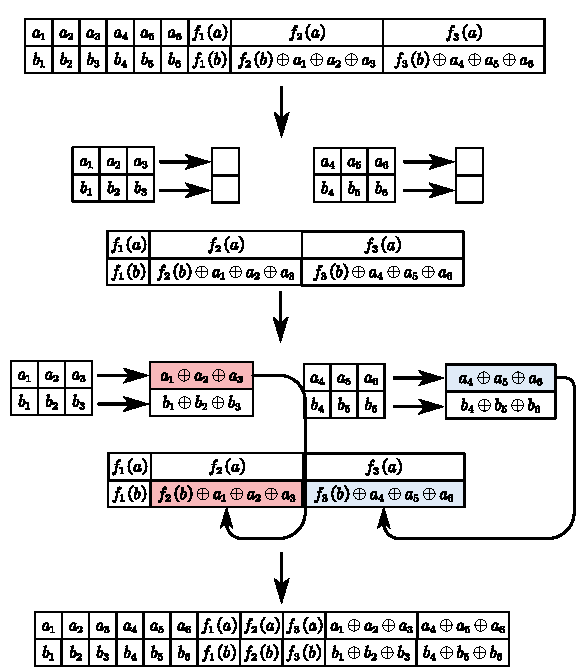
\includegraphics [scale=1.2]{figures/4.5.pdf}
	\caption{HH$(6,3) \rightarrow $ LRC$(6,2,3) $过程}
	\label{fig:4.5}
\end{figure}

\section{实验结果与分析}

\subsection{实验参数与数据集}

实验选取参数的$(k,t)=(12,4)$,即在系统中部署LRC$(12,3,4)$和HH$(12,4)$两种编码。根据这一选择,在仿真平台上
需要19个以上的节点部署,其他实验环境与第\ref{chapter:3}章一致。本文选择了四种数据集\cite{narayanan2008write}作为经典的系统运行负载如表~\ref{table:4-3}
所示,
关于每个数据集的解释如下:

\begin{itemize}
	\item \textsc{MSR-mds1},来自于媒体服务器且在四个数据集中拥有最高的读取比例;
	\item \textsc{MSR-rsrch0,MSR-rsrch2},两个数据集均通过研究项目产生,其中\textsc{MSR-rsrch0}的读取量最低,且\textsc{MSR-rsrch2}含有中等的读取量数据;
	\item \textsc{MSR-web1},通过Web/SQL服务器产生,拥有中等的读取数据量。
\end{itemize}

\begin{table}[htbp]
	% \setlength{\tabcolsep}{2.9pt}
	\centering
	\caption{数据集介绍}
	\begin{tabular}{llrlr}
		\toprule
		\textsc{数据集}     & 请求数    & 读取比    & IOPS    & 平均请求数据大小    \\[1pt]
		\midrule
		\\[-15pt]
		\textsc{MSR-mds1}                      & 1637711              & 92.88\%              & 27.29           & 113.00KB     \\
		\textsc{MSR-rsrch2}                      & 207597              & 65.69\%               & 3.54           & 8.17KB           \\
		\textsc{MSR-web1}                      & 160891              & 54.11\%               & 2.66           & 58.14KB           \\
		\textsc{MSR-rsrch0}                      & 1433655              & 9.32\%              & 23.70           & 17.86KB       \\
		\bottomrule
	\end{tabular}
	\label{table:4-3}
\end{table}



对于修复负载,在实验平台中随机初始化故障事件,然后记录故障节点的位置和时间戳。对于时间间隔的处理,计算从最后一次
发生故障的时间间隔,并通过输入的时间间隔生成满足正态分布故障概率的故障事件。对于故障位置,设置目标故障节点和
最近故障节点之间的相对距离与故障概率成反比。同样由于存储系统中98\%的故障时单节点故障\cite{xia2015tale},所以实验基于单节点故障进行。
对于\citet{wang2020adaptive}的LRC\&HH策略默认存储方式为HH码,因为他们在实验中的数据访问遵循Zipf模拟,并且没有相应的
自适应负载切换算法,所以设置为数据访问时随机切换编码策略,具体来说当数据访问产生时,随机选择是否根据当前编码策略读取数据,否则
切换为另一种编码策略从而访问数据。

此外,本文选取了四种指标作为实验结果的衡量尺度,分别为读写负载性能$\epsilon_1$,修复负载性能$\epsilon_2$,整体负载性能$\epsilon$和
临界比$\zeta$。
正如章节\ref{subsection:4.1}所分析的三种
参数的量化。具体的指标定义如下:
\begin{enumerate}
	\item 读写负载性能$\epsilon_1$,定义为读写任务中的读写操作的平均延迟,包括了计算和数据访问消耗即transmission+disk I/O;
	\item 修复负载性能$\epsilon_2$,定义为修复任务中解码操作的平均消耗,包括计算和访问消耗;
	\item 整体负载性能$\epsilon$,定义为$\epsilon=\frac{\mu_1\epsilon_1 + \mu_2\epsilon_2}{\mu_1 + \mu_2}$,这里$\mu_1$和$\mu_2$分别代表读写和修复中的请求数;
	\item 临界比$\zeta$,定义为$\zeta = \frac{1}{\epsilon \times \rho}$,表示性能优先和存储优先之间的比例,其中$\rho = \frac{k+r}{k}$。
\end{enumerate}

\subsection{读写负载性能实验结果}


在读写负载性能实验中,RS$(10,4)$在四个数据集上的的修复时间都略高于HH$(10,4)$和LRC$(12,2,3)$的方案。
其中LRC$(12,2,3)$构建的方案比HH$(10,4)$的修复速度更快一点。而利用了二者优势的LRC\&HH Random码,在重建性能
上远优于二者,这是由于在系统上冷热数据转换时,会将LRC$(k,t-1,t)$切换为HH$(k,t)$,原本的切换方式需要
传递$(k+t-1)$个块,而混合方案只需要传输$(t-1)$个子块,即$\frac{t-1}{2}$,而当$k=12$且$t=4$时,这种切换
算法只需要重新编码算法的$\frac{1}{10}$。反过来,冷数据转换为热数据时,会将HH$(k,t)$切换为LRC$(k,t-1,t)$,
若重新编码则需要传输$(t+2t-2)$个块,而切换算法只需要传输$(2k+t-1)$个子块,即$\frac{2k+t-1}{2}$块,当
$k=12$且$t=4$时,传输的数据量为原来的$\frac{1}{4}$。

在这基础上,本文算法在四个数据集上平均性能比LRC\&HH Random又有了相应的优化,平均修复时间降低了18.7\%。因为
LRC\&HH Random在存储系统的读取与修复过程中没有对数据的自适应转换做相应的优化,本文策略在读写负载上,
利用队列技术以及相应的计算分析出了负载均衡点,从而可以从图~\ref{fig:4-6}中的蓝色柱子看出,本文的策略在前三个数据集上的
优化较为明显,因为其相应的读取比很高。

\begin{figure}[htbp]
	\centering
	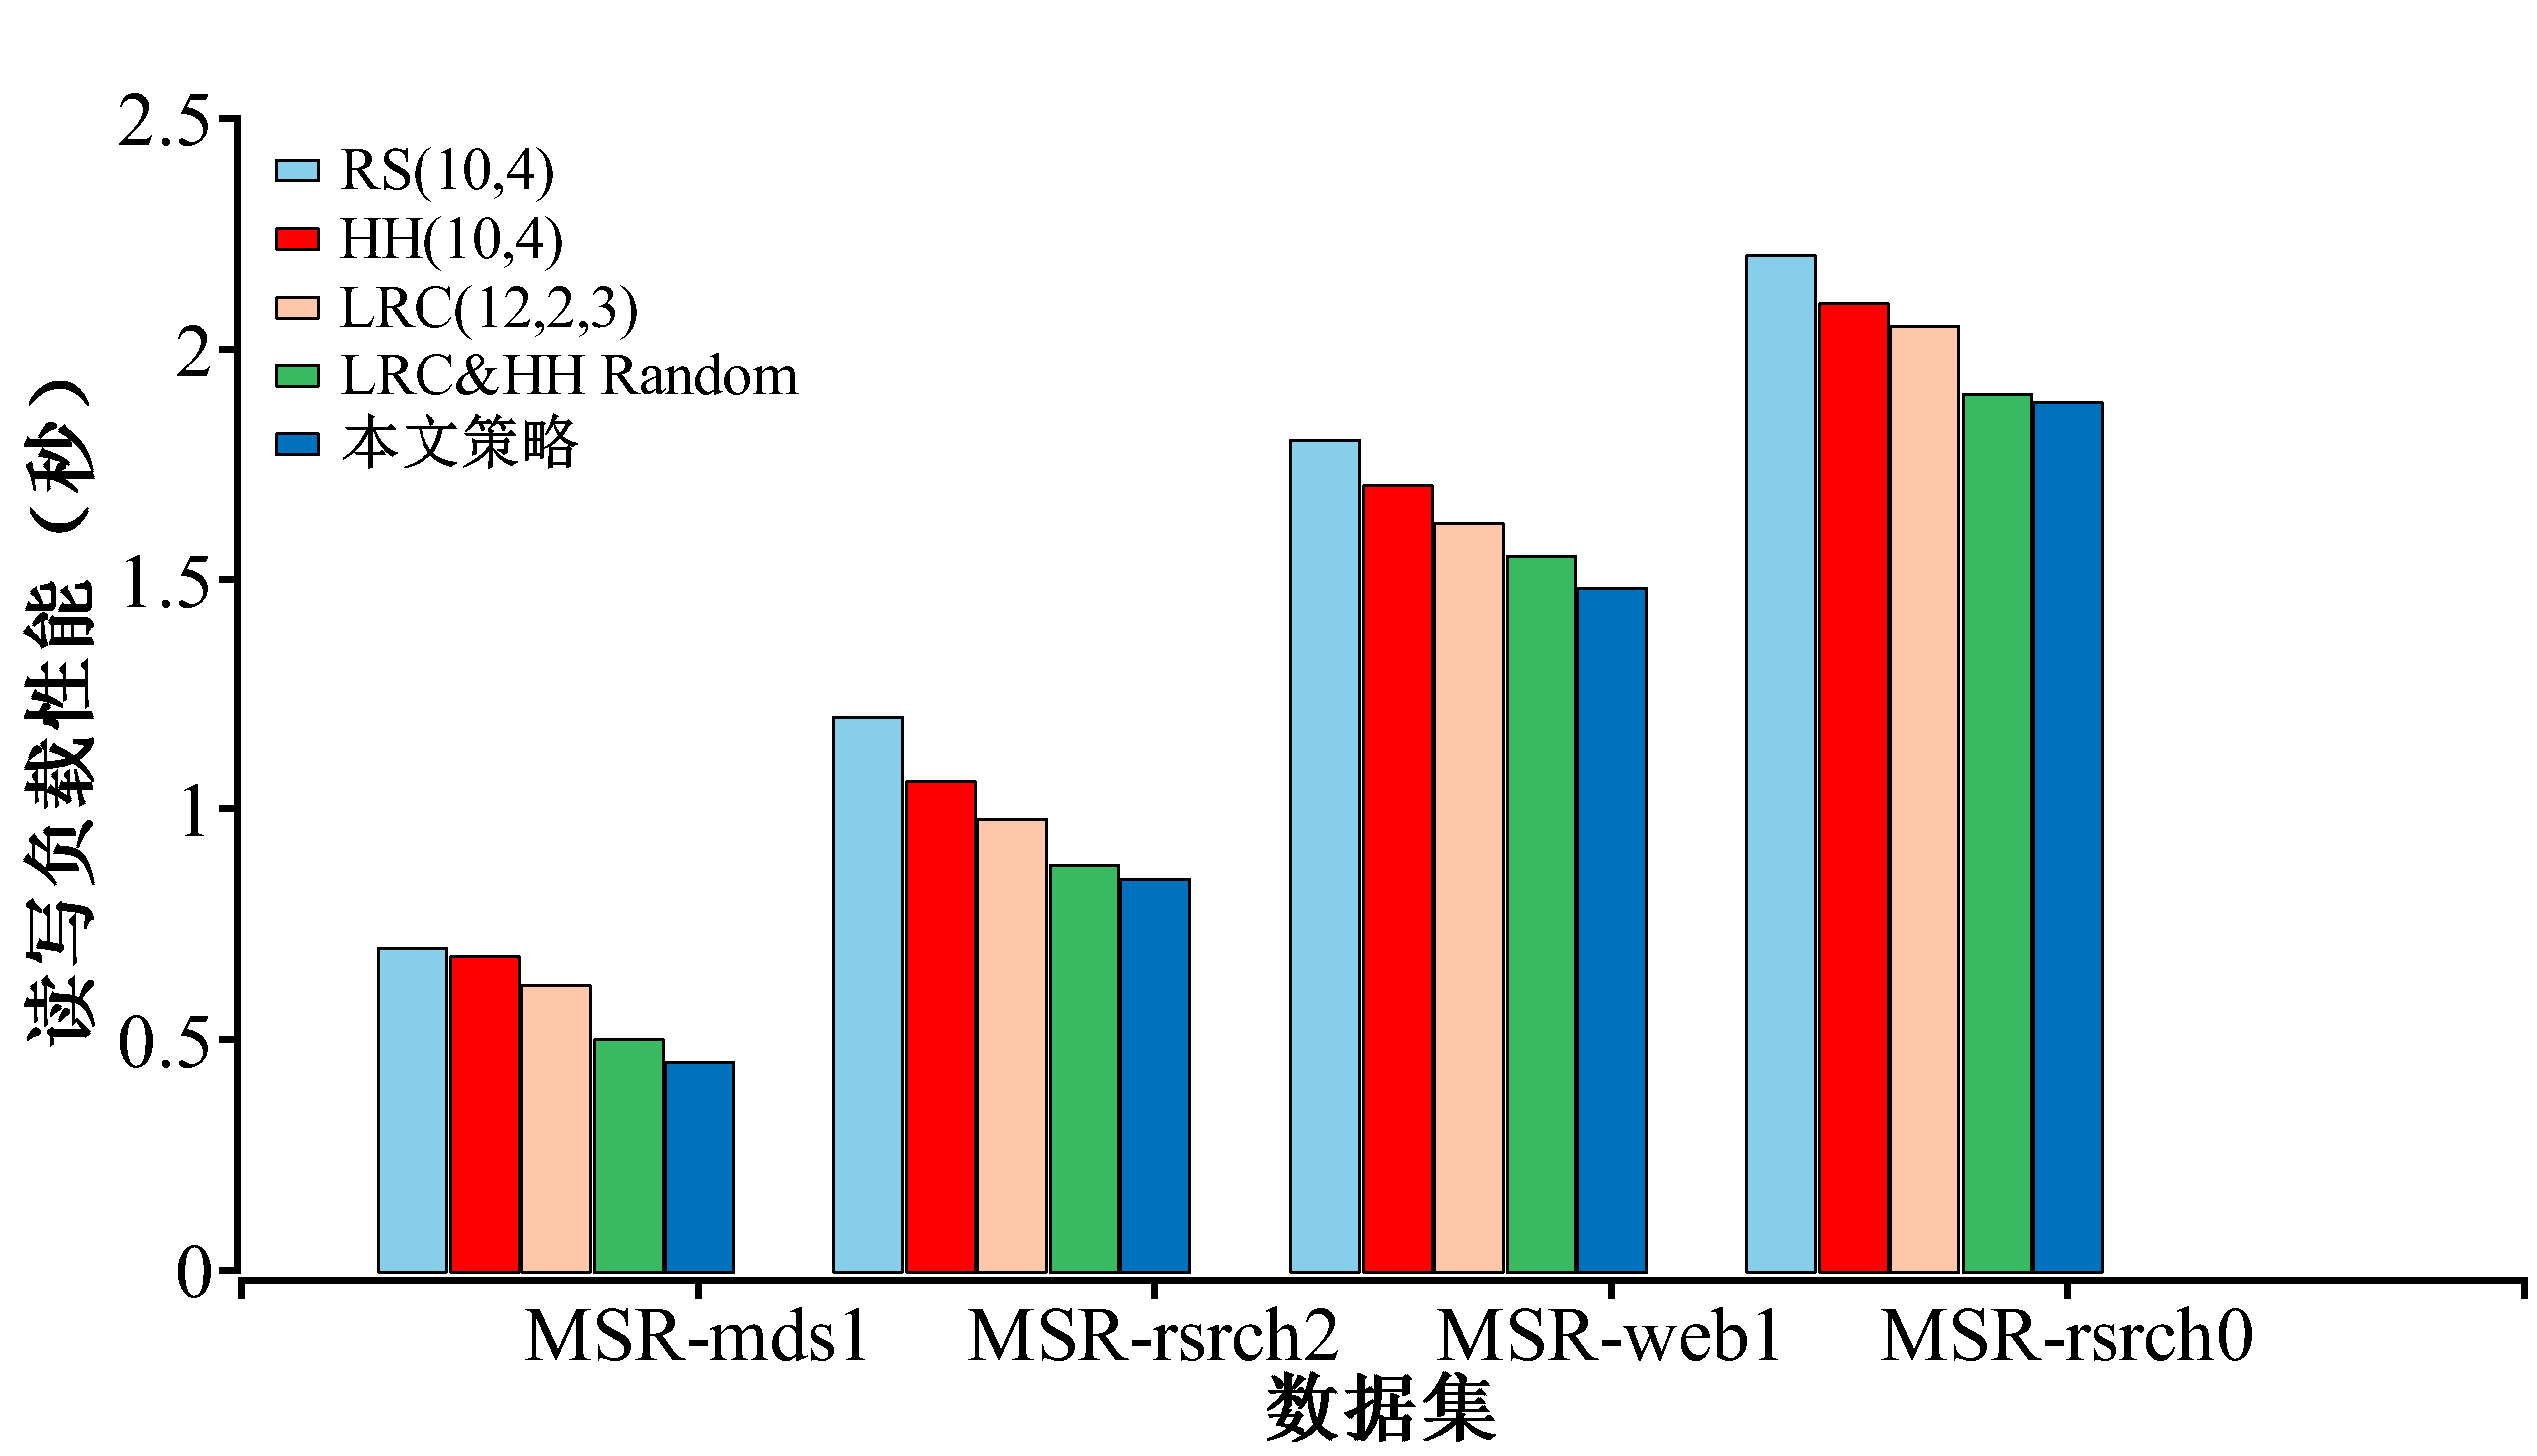
\includegraphics [scale=0.25]{figures/4-6.pdf}
	\caption{四个数据集的读写负载性能实验}
	\label{fig:4-6}
\end{figure}


\subsection{修复负载性能结果}

与读写负载实验相比,四个数据集的修复负载实验中的结果的差异化更加明显。其中,RS$(10,4)$在四个数据集上都表现出了远超于
其他方案的修复时间,主要是修复负载下,热数据的冗余更多,而RS$(10,4)$消耗了巨大的计算性能,从而拉高了修复时间。在\textsc{MSR-mds1}中,
LRC\&HH Random与本文策略的修复时间差距不大,主要是由于其具有较大的请求数、读取比以及IOPS,这样的高度集中的数据请求的情况下,
算法不能做出及时的反应。而在其他三个数据集\textsc{MSR-web1}、\textsc{MSR-rsrch2}以及\textsc{MSR-rsrch0},本文策略都用较为明显的优势,在平均性能上降低了9.4\%的修复时间。

\begin{figure}[htbp]
	\centering
	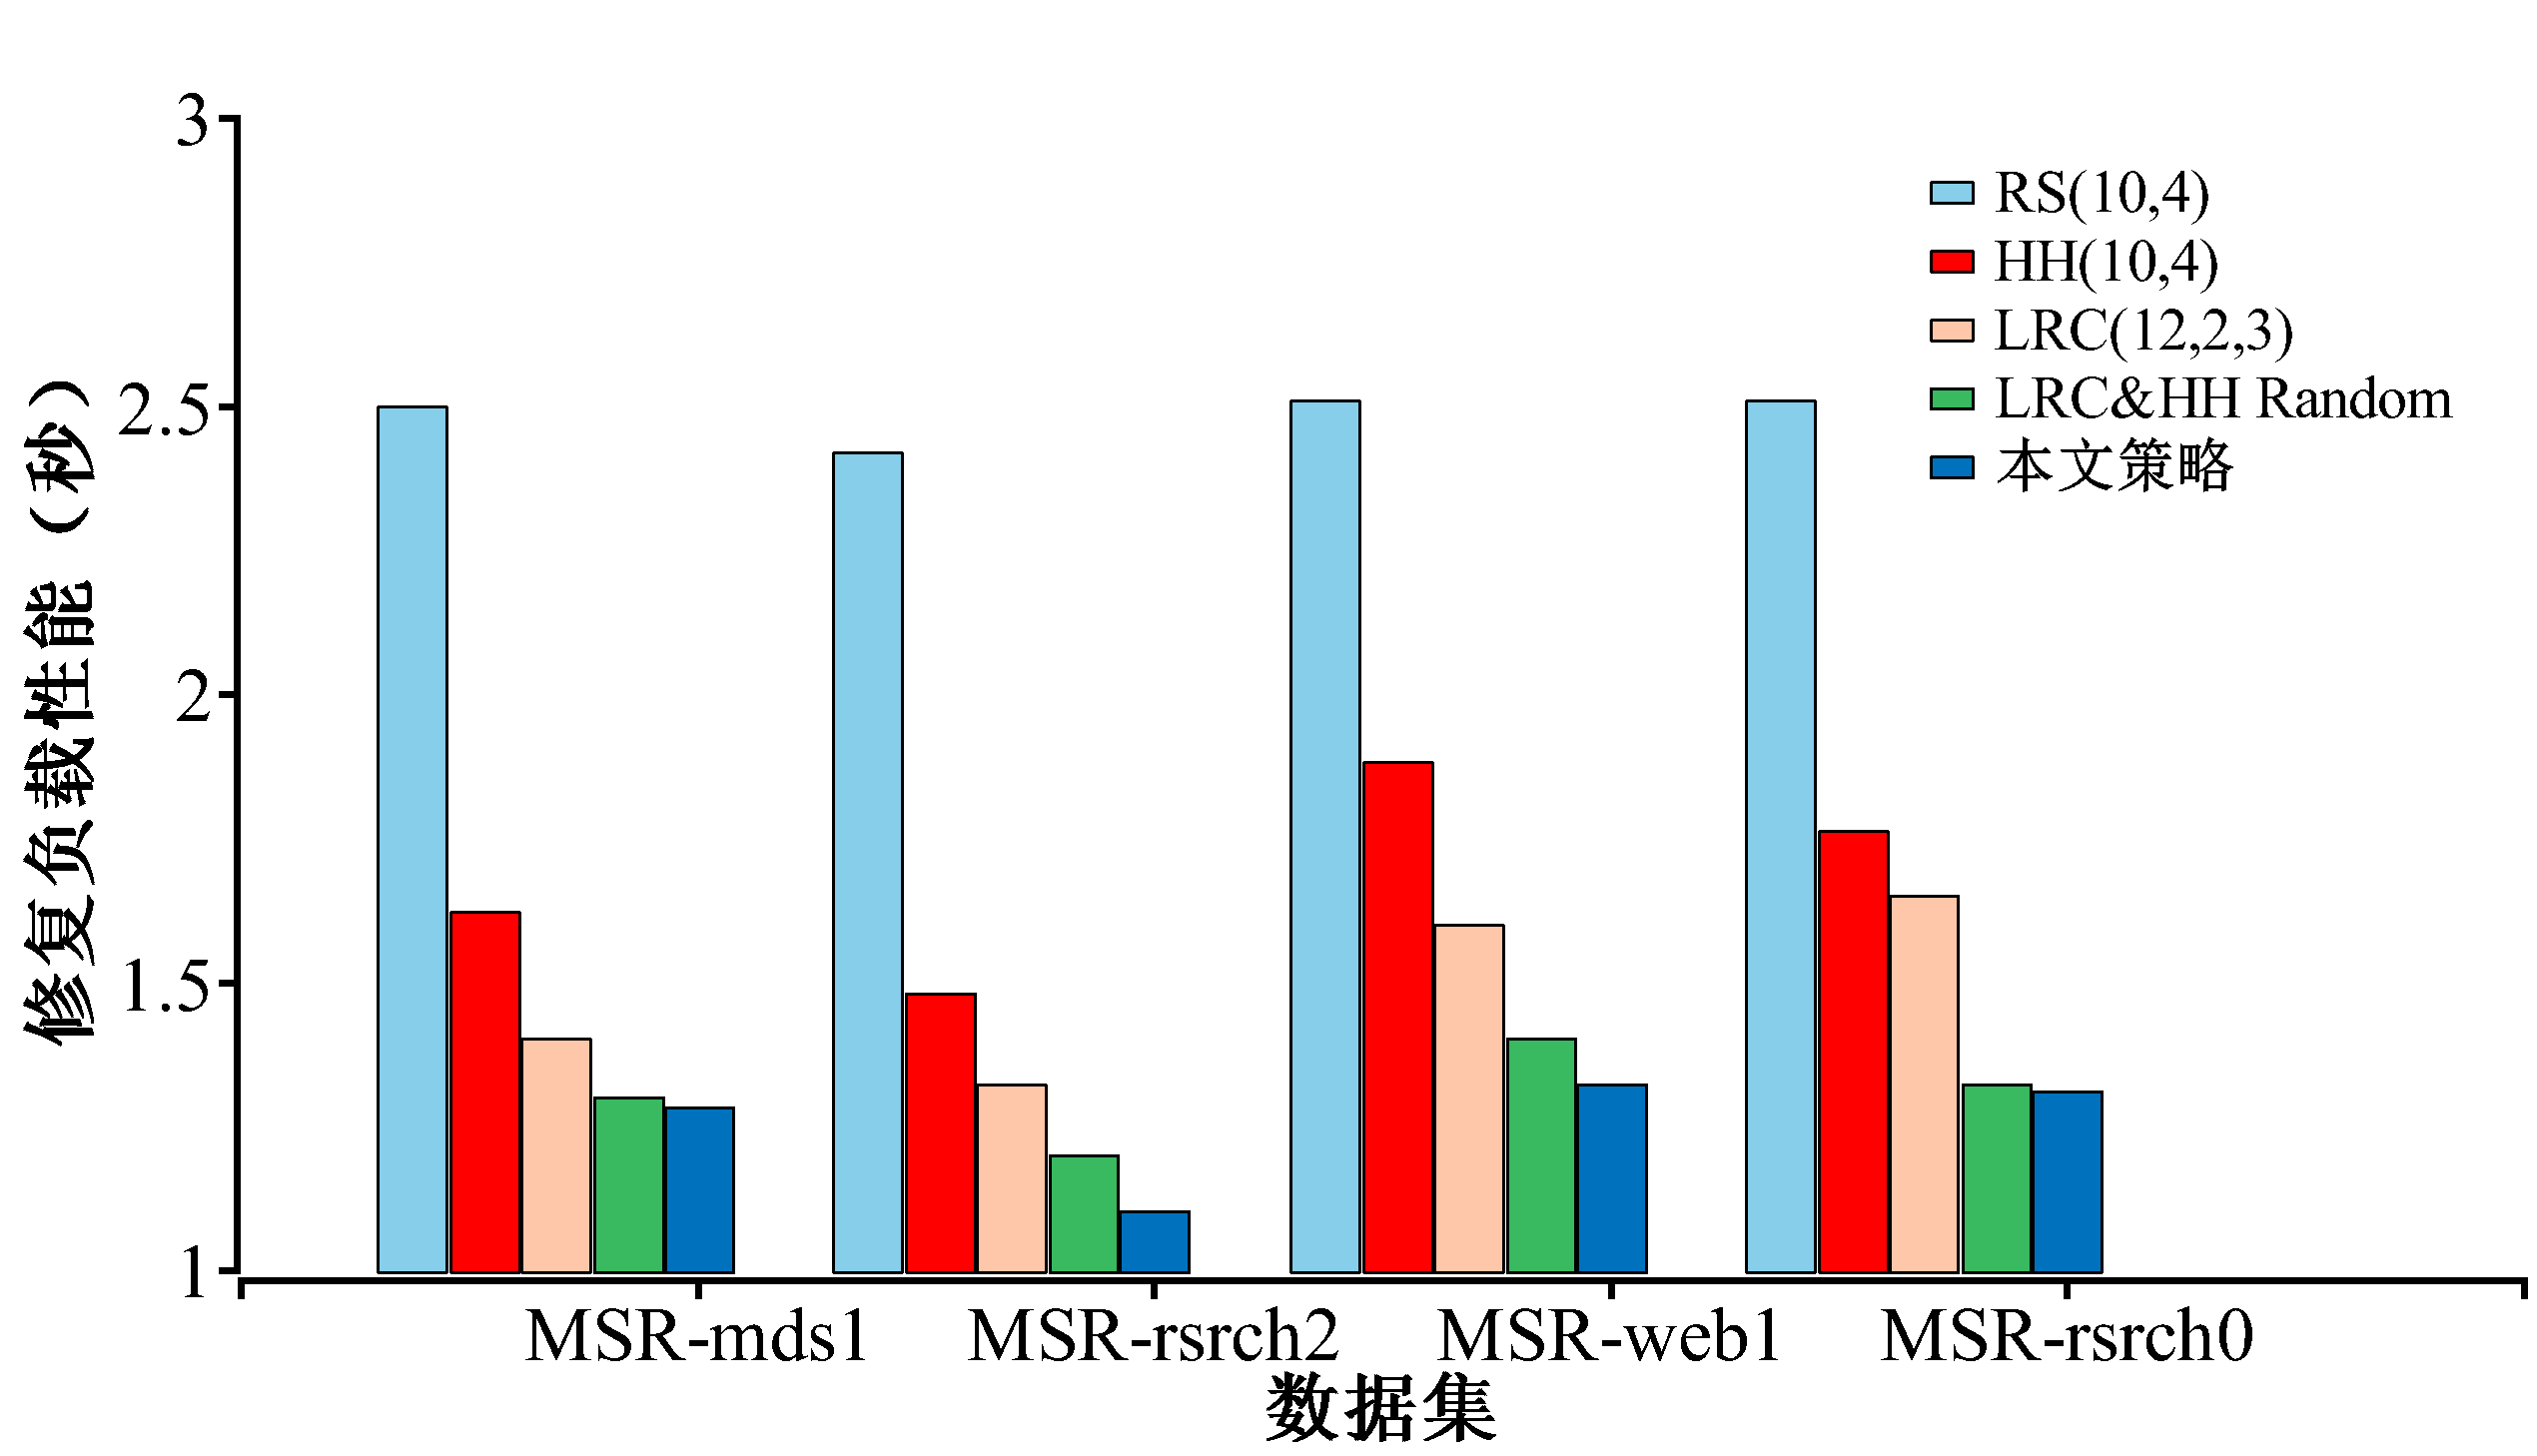
\includegraphics [scale=0.25]{figures/4-7.pdf}
	\caption{四个数据集的修复负载性能实验}
	\label{fig:4-7}
\end{figure}



\subsection{整体负载性能实验结果}


在整体性能实验中,即将读写和修复任务均匀地分摊到系统事件中,从而观察各个策略的修复性能。从图~\ref{fig:4-8}可以看出,在
读写和修复交叉的任务中,RS$(10,4)$在不同数据集上的修复性能有所上升。此外HH$(10,4)$和LRC$(12,2,3)$在不同数据集上的差异
很小,在\textsc{MSR-rsrch0}上,HH$(10,4)$的修复时间最高,且LRC\&HH Random的平均性能还是会优于其他的单一纠删码,因为
在整体负载情况下,切换任务时有发生。但是由于切换时机的随机性,本文策略在基于实时的冷热数据优化算法以及自适应策略的帮助下,
在大部分情况下依然优于随机切换的方式,平均性能上降低了6.8\%的修复时间。此外,在计算效率方面,这两种策略都是进行XOR运算,
且涉及范围相对整一组数据较小,这对比重新编码算法需要整份数据进行的伽罗瓦运算也有了明显的优化,大大提升了计算效率。


\begin{figure}[htbp]
	\centering
	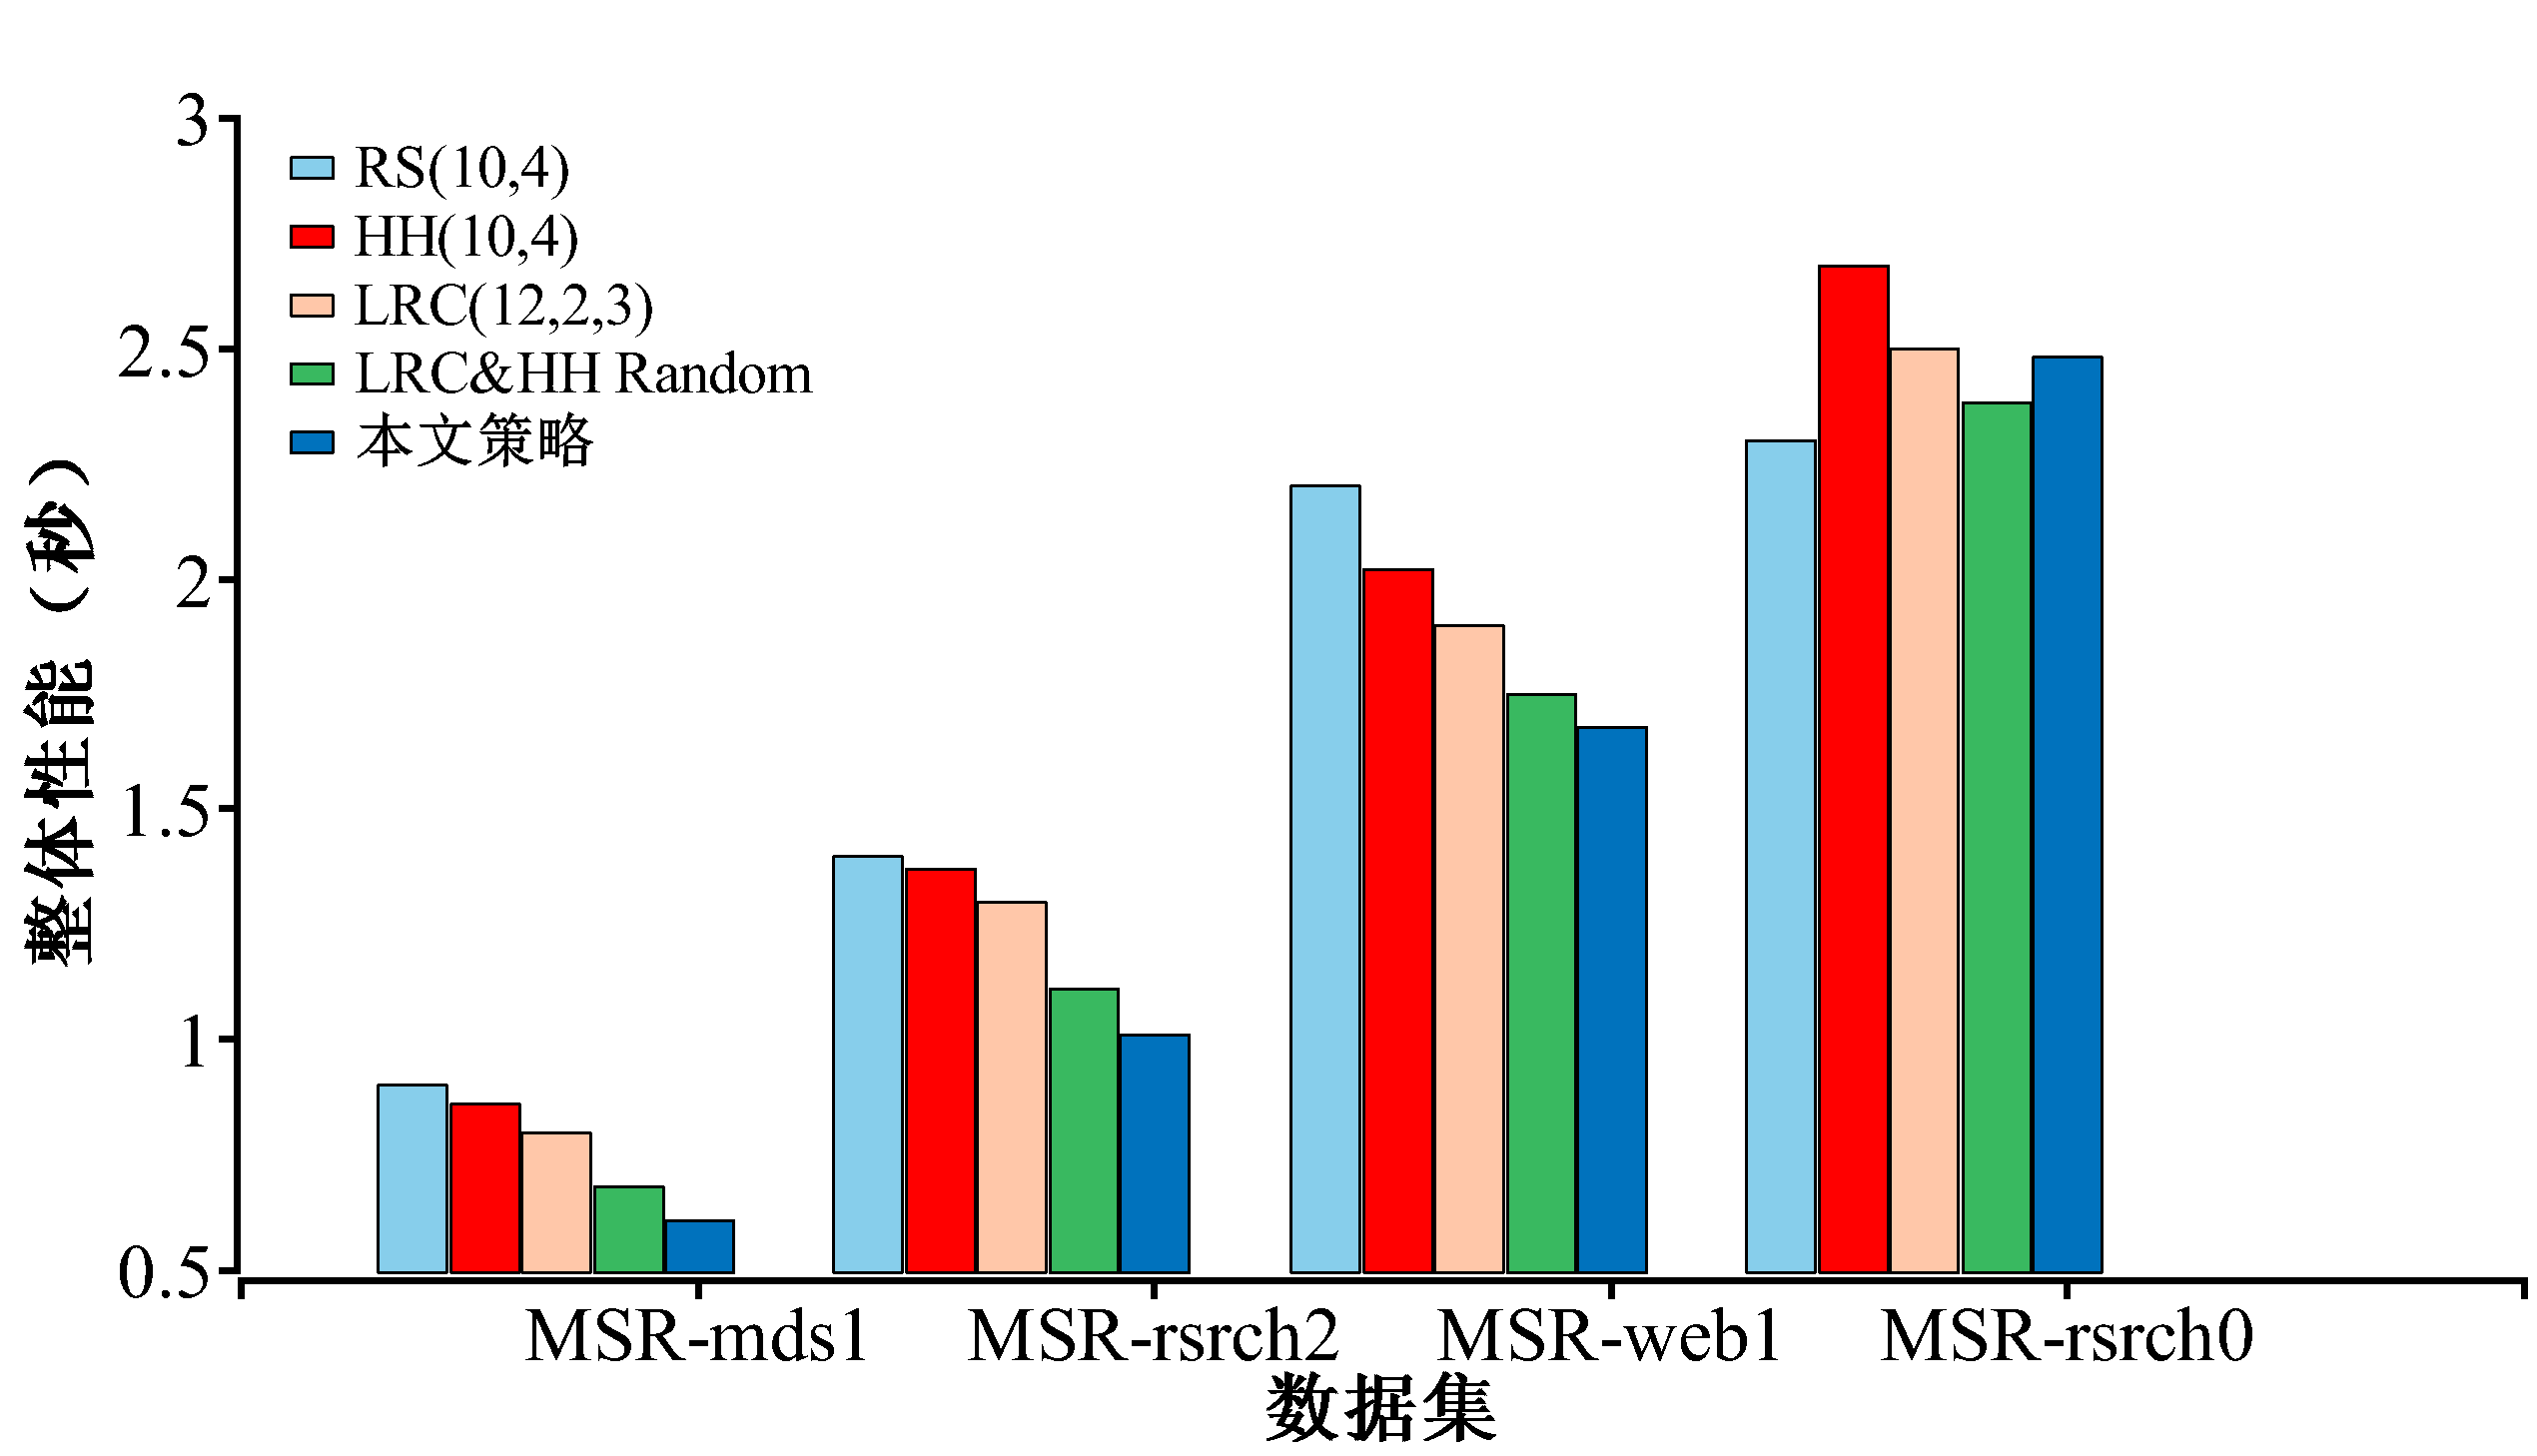
\includegraphics [scale=0.2]{figures/4-8.pdf}
	\caption{四个数据集的整体负载性能实验}
	\label{fig:4-8}
\end{figure}

\subsection{临界比实验结果}

临界比是一种衡量修复消耗的参数,数值越低则代表具有相应更低的修复消耗,修复性能更加优越。从图~\ref{fig:4-9}可以看出,
LRC$(12,2,3)$在四个数据集上都有着较高的临界比,意味着更加低的修复性能,与之相类似的是HH$(10,4)$,在前两个数据集上的
数值基本下基本相同。在平均性能上,本文策略的临界比相较于LRC\&HH Random低5.8\%。

\begin{figure}[htbp]
	\centering
	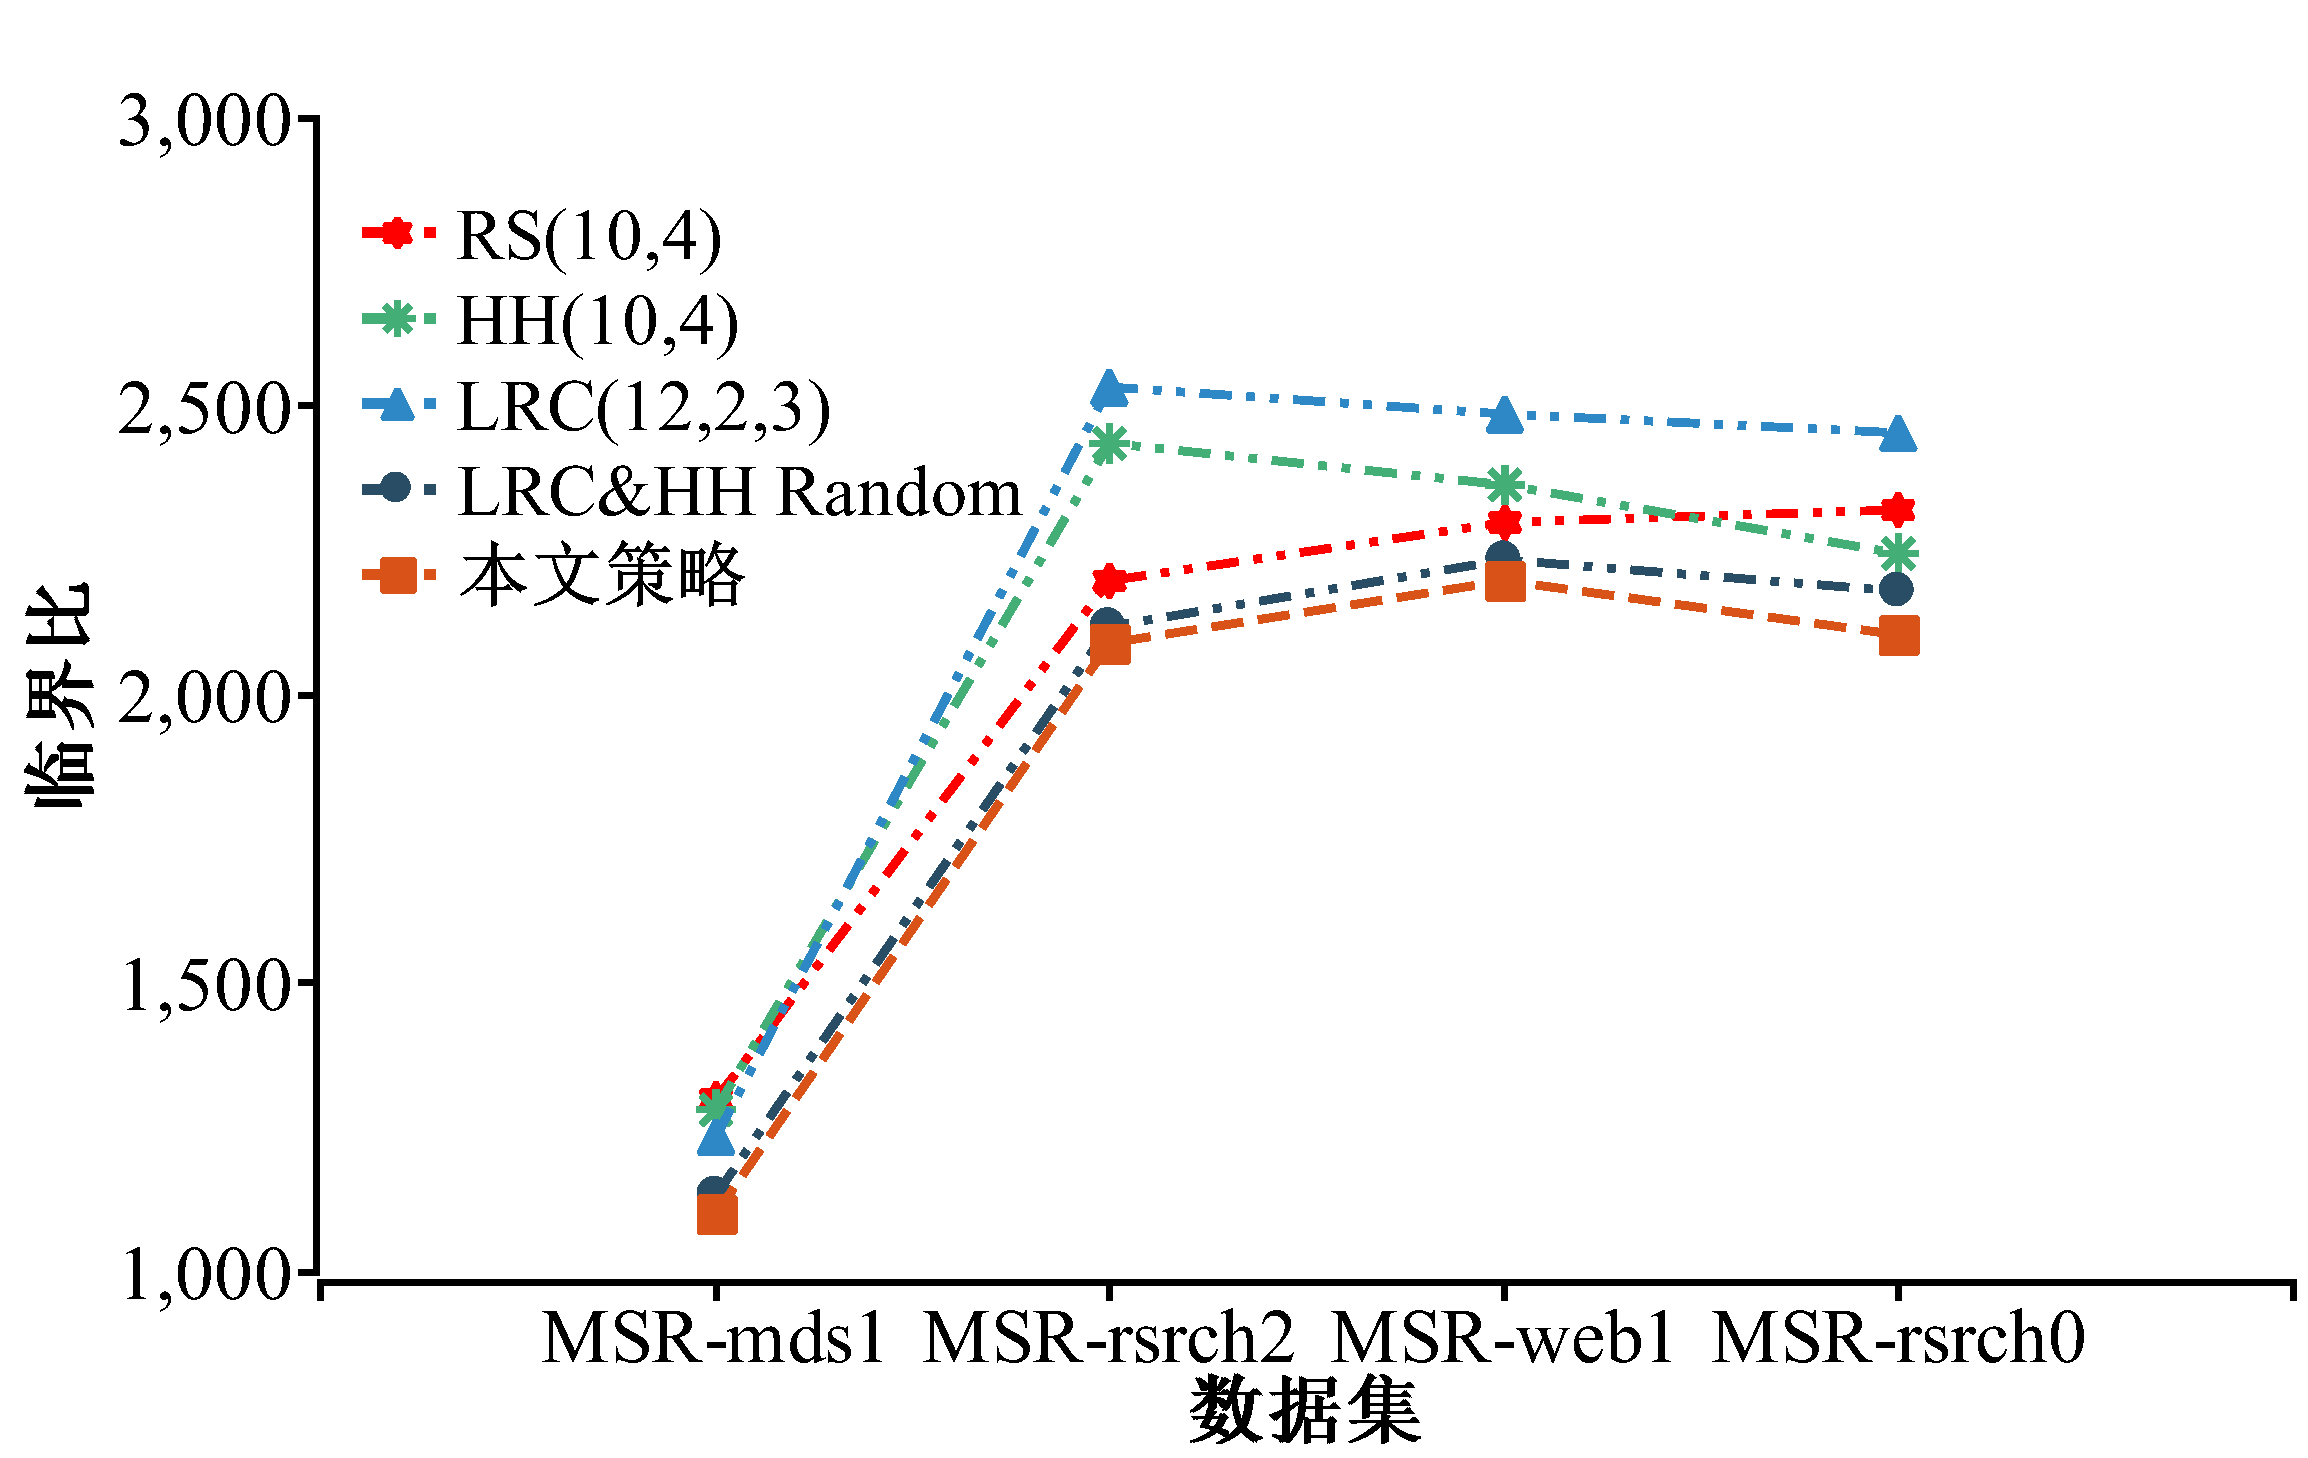
\includegraphics [scale=0.25]{figures/4-9.pdf}
	\caption{四个数据集的临界比实验}
	\label{fig:4-9}
\end{figure}


\section{本章小结}
针对在传统的存储系统中大多只采用一种纠删码进行数据的处理和存储,难以在保持低存储空间消耗的情况下降低退化读的延迟时间问题。
本文在前文预先修复的单一纠删码的基础上,进一步推进了纠删码修复技术的
应用,提出了一种可感知数据热度的负载动态自适应
的混合纠删码(LRC\&HH)数据修复方案。静态地将数
据分为六类,分别根据读写负载平衡和修复负载,根据数学计算提出相应的负载均衡策略,使用
LRU 算法来为冷热数据划分定制自适应选择算法。选取四个数据集,分别对读写负载,修复负载,
整体负载和临界比进行了对比实验,实验结果表明,
本文策略相较于LRC\&HH Random降低了6.8\%$\sim$18.7\%的修复时间。
% \chapter{总结与展望}
\chapter{基于预测修复的纠删码存储系统原型设计与实现}
\chapter{总结与展望}
\section{论文工作总结}

分布式存储系统通常采取存储超过原本数据1倍的冗余数据来保证数据
可靠性以对抗节点故障而导致的数据丢失,进而通过冗余数据进行相关的计算还原
出丢失的数据。但无论是多副本技术还是纠删码方式都会产生冗余数据,并且都有其固有的缺陷。
本文主要对基于纠删码构建的存储系统的数据修复技术进行了研究实验,受到系统带宽性能和计算性能的影响,
数据修复技术要综合考虑修复延迟,数据重建,修复块传输,带宽变化等多方面因素。本文在传统反应式修复
的基础上改进了重建与迁移修复的传输方式,并且结合混合纠删码的策略以及相应的自适应算法完成对基于
纠删码构建的存储系统的数据修复技术研究。现对本文的工作总结如下:

纠删码面临的最基本问题就是过量的修复开销:修复流量随着存储冗余度的降低
而增加。目前,大部分的传统修复方法都
是被动修复,只有在检测到节点故障后才会触发修复操作。如果可以提前预测即将发
生的故障,就可以在任何实际故障发生之前主动修复任何即将发生的节点故障,以提
高系统可靠性。针对上述问题,本文通过结合迁移与重建来设计实现预先修复的机制,用以修复 STF(Soon To
Fail)节点。首先,本文针对重建集与迁移集问题,设计了划分迁移集与重建集算法
SMSRS(Split Migration Set And Reconstruction Set)算法,该算法主要
使用数据热度队列与最小堆技术,根据数据访问热度高低处理待修复的块的出队修
复顺序,利用最小堆不断优化当前出堆的网络带宽性能最优的可用节点进行迁移修
复,然后通过贪心策略确定最佳的重建节点以及对应的重建块接收节点。其次,
本文提出了ISA(Improved SMFRepair Algorithm)算法来
进行节点修复的调度。通过加入空闲节点(idle nodes)进行数据中继的方式可以对传输问题进一步优
化。IBA在每一轮修复中首
先判断该任务是迁移还是重建,根据输入参数进行确认,采用局部最优
修复,在此过程中链路带宽不断发生变化,从而实现最优化。
通过调整系统总节点数,RS码配置,磁盘带宽,网络带宽,条带数,块大小,空闲节点数等实验因素,
实验结果表明,本文算法相较于传统的FastPR有着一定程度的改善,修复时间降低了7.2\%$\sim$13.2\%。

在传统的存储系统中大多只采用一种纠删码进行数据的处理和存储,然而这种方
式难以在保持低存储空间消耗的情况下降低退化读的延迟时间。
本文在前文预先修复的单一纠删码的基础上,进一步提出了一种可感知数据热度的负载动态自适应
的混合纠删码(LRC\&HH)数据修复方案。针对实际存储系统数据I/O的特点,将不同的数据进行分类,并且
为了让不同的数据和读写任务工作负载情况匹配上适当的编码方案通过理论定量计算区分了读写负载模式和
修复负载模式下的纠删码修复方案。根据相应的两种纠删码的切换算法,选取四个数据集,分别对读写负载,修复负载,
整体负载和临界比进行了对比实验,实验结果表明,
本文策略相较于LRC\&HH Random降低了6.8\%$\sim$18.7\%的修复时间。

为了验证预先修复技术和混合纠删码修复技术在实际应用中的性能,本章设计
并实现了一个容错存储原型系统。该系统有三个特点:(1)基于开源分布式存储中心
的离散事件模拟器 SimEDC 进行设计实现;(2)含有丰富的混合纠删码方案,包括
已有的 HACFS 、EC-Fusion以及LRC\&HH,支持相应的扩展接口;(3)支
持修复调度中的重建与迁移的融合。容错存储原型系统设计主要包含以下模块:存储中心架构,节点故障模型,混合
纠删码策略,节点放置策略,可靠性度量指标,事件处理模式。实验结果表明,基于混合纠删码结构的容错存储原型系统具有较高的可靠性,
PDL参数平均降低了30\%$\sim$35\%,NOMDL平均
降低了40\%$\sim$42.5\%,BR平均降低了35.6\%$\sim$37.8\%。


\section{未来工作展望}
本文主要针对基于纠删码构建的存储系统中的预先修复技术和混合纠删码技术进行了研究实验,提出了
重建划分算法和修复调度算法以及混合纠删码的自适应算法。
但是,本文针对的修复任务是单节点的修复任务,并未涉足于多节点的修复任务,在之后的研究中,需要
将相应的技术扩展到多节点的并行修复任务中,提升系统的可靠性。


% % \begin{table}[htbp]
%     \centering
%     \caption{BEBG的相对消息冗余RMR}
%     \begin{tabular}{lccccccc}
% 		\toprule
%         N/$f_\text{out}$(BEBG,NHDG) & 2 & 3 & 4 & 5 &6 &7 & 8 \\[1pt]
%         \midrule
%         \\[-15pt]
%         100         & 1.78/0.79         & 4.41/3.82         & 5.91/7.93         & 8.66/12.13          & -                   & -                 & -              \\
%         1000        & -                 & 3.72/3.89         & 6.14/7.99         & 8.76/12.66          & 11.42/15.02         & 14.45/21.98       & -              \\
%         10000       & -                 & -                 & 6.12/7.98         & 8.49/13.99          & 11.13/15.37         & 13.78/21.36       & 16.99/28.41    \\
%     \bottomrule
%     \end{tabular}
%     \label{table:3-dup_BEBG}
% \end{table}
\begin{table}[htbp]
    \centering
    \caption{BEBG的相对消息冗余RMR}
    \begin{tabular}{lccccccc}
		\toprule
        N/$f_\text{out}$(BEBG) & 2 & 3 & 4 & 5 &6 &7 & 8 \\[1pt]
        \midrule
        \\[-15pt]
        100         & 1.78         & 4.41         & 5.91         & 8.66          & -             & -           & -        \\
        1000        & -            & 3.72         & 6.14         & 8.76          & 11.42         & 14.45       & -        \\
        10000       & -            & -            & 6.12         & 8.49          & 11.13         & 13.78       & 16.99    \\
    \bottomrule
    \end{tabular}
    \label{table:3-dup_BEBG}
\end{table}
% \begin{table}[htbp]
    \centering
    \caption{NHDG的相对消息冗余RMR}
    \begin{tabular}{lccccccc}
		\toprule
        N/$f_\text{out}$(NHDG) & 2 & 3 & 4 & 5 &6 &7 & 8 \\[1pt]
        \midrule
        \\[-15pt]
        100         & 0.79         & 3.82         & 7.93         & 12.13          & -             & -           & -        \\
        1000        & -            & 3.89         & 7.99         & 12.66          & 15.02         & 21.98       & -        \\
        10000       & -            & -            & 7.98         & 13.99          & 15.37         & 21.36       & 28.41    \\
    \bottomrule
    \end{tabular}
    \label{table:3-dup_NHDG}
\end{table}
% \begin{table}[tb!]
	\centering
	\caption{Test数据的结果.}
	\begin{tabular}{cccccccc}
		\toprule
		$f_{out}$ & \multicolumn{3}{c}{$f_{out}(BEBG)$} & \multicolumn{3}{c}{$f_{out}(NHDG)$}                                      \\
		$N$       & $100$                               & $1000$                              & $10000$ & $100$ & $1000$ & $10000$ \\
		\midrule
		2         & 1.78                                & -                                   & -       & 0.79  & -      & -       \\
		3         & 4.41                                & 3.72                                & -       & 3.82  & 3.89   & -       \\
		4         & 5.91                                & 6.14                                & 6.12    & 7.93  & 7.99   & 7.98    \\
		5         & 8.66                                & 8.76                                & 8.49    & 12.13 & 12.66  & 13.99   \\
		6         & -                                   & 11.42                               & 11.13   & -     & 15.02  & 15.37   \\
		7         & -                                   & 14.45                               & 13.78   & -     & 21.98  & 21.36   \\
		8         & -                                   & -                                   & 16.99   & -     & -      & 28.41   \\
		\bottomrule
	\end{tabular}
	\label{table:con-test}
\end{table}


% \begin{table}[tb!]
	\centering
	\caption{(n个)}
	\begin{tabular}{lcccc}
		\toprule
		字段名称      & 数据类型     & 主键 & 是否空 & 说明             \\[1pt]
		\midrule
		\\[-15pt]
		user$\_$code  & varchar(50)  & Y    & N      & 主键,用户标识ID \\
		user$\_$name  & varchar(20)  & N    & N      & 用户名           \\
		password      & varchar(20)  & N    & N      & 密码             \\
		user$\_$email & varchar(50)  & N    & N      & 邮箱             \\
		public$\_$key & mediumtext   & N    & N      & 公钥             \\
		comment       & varchar(255) & N    & N      & 备注信息         \\
		\bottomrule
	\end{tabular}
	\label{table:5-1}
\end{table}





% % 参考文献,4或者小4楷体
\addcontentsline{toc}{chapter}{参考文献}
\begin{kai}
  \bibliography{reference}
\end{kai}

% % 附录,4或者小4楷体
% \appendix

% 附页标题样式
\backmatter
% 附页
\chapter{攻读学位期间的成果}

\begin{itemize}
	\setlength{\itemsep}{5pt}
	% \setlength{\parsep}{2em}
	
	\item \textbf{\heiti\sihao{论文}}
	      \begin{enumerate}
			% \renewcommand{\labelenumi}{\[\theenumi\].}
	      	\setlength{\itemsep}{-\itemsep}  %调整间距
	      	% \usecounter{numcount} % 使用计数器,初始值为0
	      	% \setlength{\leftmargin}{3em} %左边界
	      	% \setlength{\parsep}{-0.5ex} %段落间距
	      	% \setlength{\topsep}{-10ex} %列表到上下文的垂直距离
	      	% \setlength{\itemsep}{0.5ex} %条目间距
	      	% \setlength{\labelsep}{0.3em} %标号和列表项之间的距离,默认0.5em
	      	% \setlength{\itemindent}{1.1em} %标签缩进量
	      	% \setlength{\listparindent}{0em} %段落缩进量
	      	\item 叶冬冬. 基于纠删码的存储系统中高可靠预测修复客户端软件,计算机软件著作权,未发表,登记号:2022SR0208709.
	      	\item 叶冬冬. 基于纠删码的存储系统中高可靠预测修复服务端软件,计算机软件著作权,未发表,登记号:2022SR0208720.
	      	% \item \textbf{第一作者}. ***,计算机软件著作权,未发表,登记号:***.
	      	% \item \textbf{第一作者}. ***,计算机软件著作权,未发表,登记号:***.
	      	% \item 小型微型计算机系统.2022.外审中. \textbf{第一作者}(对应论文第三章)
	      	% \item 计算机应用与软件.2022.外审中. \textbf{第一作者}(对应论文第四章)
	      	\item 计算机系统应用.2022.外审中. \textbf{第一作者}
			  % \item \textbf{Yu Zhang}, Zhenghua Li, Min Zhang. 2020.
	      	%       \emph{Efficient Second-Order TreeCRF for Neural CRF Dependency Parsing}.
	      	%       In Proceedings of ACL, pages 3295–3305, Online. (CCF-A类会议)
	      	% \item \textbf{Yu Zhang}$^\ast$, Houquan Zhou$^\ast$, Min Zhang. 2020.
	      	%       \emph{Fast and Accurate Neural CRF Constituency Parsing}.
	      	%       In Proceedings of IJCAI, pages 4046-4053, Online. (CCF-A类会议)
	      	% \item Houquan Zhou$^\ast$, \textbf{Yu Zhang}$^\ast$, Zhenghua Li, Min Zhang. 2020.
	      	%       \emph{Is POS Tagging Necessary or Even Helpful for Neural Dependency Parsing?}.
	      	%       In Proceedings of NLPCC. pages 179-191, Zhengzhou, China (CCF-C类会议, \textbf{\textit{Best Paper Award}})
	      	% \item Wei Jiang, Zhenghua Li, \textbf{Yu Zhang}, Min Zhang. 2019.
	      	%       \emph{HLT@SUDA at SemEval 2019 Task 1: UCCA Graph Parsing as Constituent Tree Parsing}.
	      	%       In Proceedings of SemEval, pages 11–15, Minneapolis, Minnesota, USA.
	      \end{enumerate}
	      
	\item \textbf{\heiti\sihao{比赛}}
	      \begin{enumerate}
	      	\item 第十七届中国研究生数学建模竞赛,二等奖.
	      \end{enumerate}
	      
	% \item \textbf{\heiti\sihao{实习}}
	%       \begin{enumerate}
	%       	\item \textsc{2021/7--2021/8}. 苏州-中国农业银行-分行计算机中心.
	%       \end{enumerate}
	      
\end{itemize}



\chapter{攻读学位期间的主要科研工作}
\begin{enumerate}
	\item 国防科技创新特区支持. 江苏省高校优势学科建设资助项目. 江苏省高校自然科学研究项目,项目号(19KJA550002). 区块链存储系统, 2019-2021.
	% \item 国防科技创新特区支持. 江苏省高校优势学科建设资助项目. 江苏省高校自然科学研究项目,项目号(*****), “*******”,2019-2021.
\end{enumerate}
\chapter{致谢}

养天地正气,法古今完人.
从本科到硕士,转眼间在美丽的苏州大学校园内度过了七年的求学时光.
在这段不算短的人生旅途中,无论是学识上还是生活阅历上我都成长良多.

首先,我要感谢我的导师李正华老师.
李老师永远以饱满的热情和专注的态度面对工作和生活,永远是我以后求学和工作的一个榜样.

感谢尊敬的张民老师,张老师以高标准要求每一个学生,营造了组内浓厚专一的科研氛围.
此外,张老师敏锐的思维、渊博的知识、平易近人的风格、深深的影响了我,平时的相处让我获益良多.
感谢陈文亮老师,陈老师开朗热情,在学业上给予了我很多指导.
同样感谢周国栋、朱巧明、李寿山、洪宇、段湘煜和李军辉等苏州大学自然语言处理实验室的所有老师,各位老师严谨的治学态度和进取的专业精神是我的榜样.

感谢周厚全师弟,厚全师弟涉猎广博,热爱阅读,富有好奇心,在平时的讨论中总是能给我很多启发.
在课题研究上我们有很多合作,也取得了很多成果,希望以后继续合作,互相促进.

感谢同组的夏庆荣师兄、龚晨师姐、李英师姐和张月师姐,各位师兄师姐总是十分热心的解决我生活和研究上遇到的困难.
感谢章波、黄德朋、江心舟师兄,彭雪师姐,在我还是萌新的时候对我的帮助,以及平时对我的关照.
感谢同届的蒋炜、陆凯华、吴锟、刘亚慧同学,大家在一起互相帮助,互相进步.
感谢沈嘉钰、李嘉诚、侯洋、李帅克、周仕林、刘泽洋、李扬师弟,还有周明月、杨浩萍师妹,十分珍惜与大家相处的美好时光.

此外,还要感谢实习期间相处的王涛师兄、蒋勇师兄,以及王新宇、胡泽川、蔡炯和马欣尹同学.
特别是感谢蒋勇师兄在我实习期间对我的关照,以及在课题研究上的悉心帮助和指导.

感谢我的父母还有家人们,你们总是我心灵上的港湾和寄托,无论何时都能给我最无私的帮助.

最后,我还要感谢各位评审老师,感谢各位老师们在百忙之中抽取时间对本文进行评审,并提出宝贵的修改意见.




\includepdf[page=-]{pdf-pages/空白页.pdf}
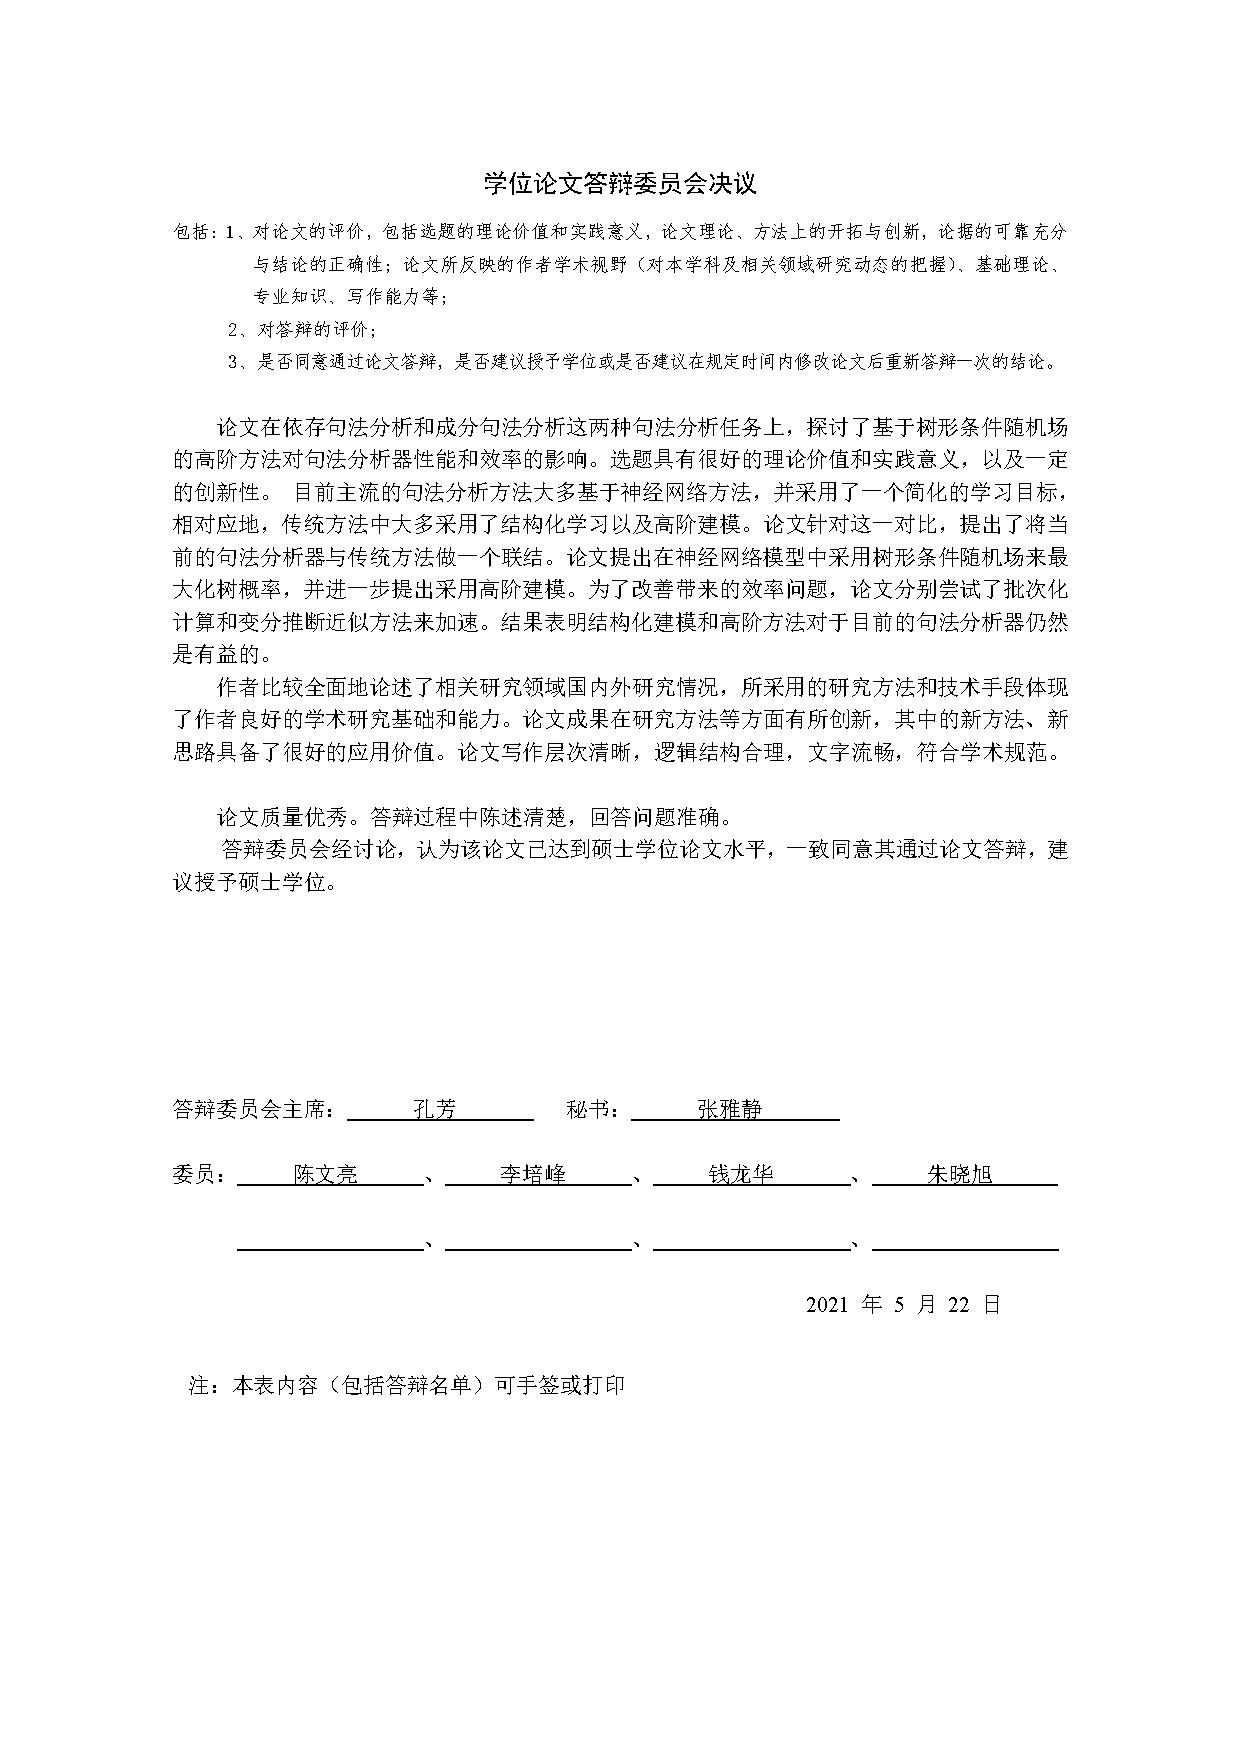
\includepdf[page=-]{pdf-pages/委员会决议.pdf}

\end{document}
